\documentclass[12pt,twoside]{report}
\usepackage{parskip}
\usepackage{comment}
\usepackage{wrapfig}
\usepackage{arev}
\usepackage[table]{xcolor}
\usepackage{gensymb}
\usepackage[export]{adjustbox}
\setlength{\parindent}{2em}  % indentation of paragraph
\usepackage{float}

\pagenumbering{arabic}

%%%%%%%%%%%%%%%%%%%%%%%%%%%%%%%%%%%%%%%%%%%%%%%%%%%%%%%%%%%%%%%%%%%%%%%%%%%%%

% Definitions for the title page
% Edit these to provide the correct information
% e.g. \newcommand{\reportauthor}{Timothy Kimber}

\newcommand{\reporttitle}{Automation and Intelligent Optimisation in High Performance Sailing Boats}
\newcommand{\reportauthor}{Doruk Taneli}
\newcommand{\supervisor}{Dr. Pedro Baiz}
\newcommand{\degreetype}{Advanced Computing}

%%%%%%%%%%%%%%%%%%%%%%%%%%%%%%%%%%%%%%%%%%%%%%%%%%%%%%%%%%%%%%%%%%%%%%%%%%%%%

% load some definitions and default packages
%%%%%%%%%%%%%%%%%%%%%%%%%%%%%%%%%%%%%%%%%
% University Assignment Title Page 
% LaTeX Template
% Version 1.0 (27/12/12)
%
% This template has been downloaded from:
% http://www.LaTeXTemplates.com
%
% Original author:
% WikiBooks (http://en.wikibooks.org/wiki/LaTeX/Title_Creation)
%
% License:
% CC BY-NC-SA 3.0 (http://creativecommons.org/licenses/by-nc-sa/3.0/)
% 
%
%%%%%%%%%%%%%%%%%%%%%%%%%%%%%%%%%%%%%%%%%
%----------------------------------------------------------------------------------------
%	PACKAGES AND OTHER DOCUMENT CONFIGURATIONS
%----------------------------------------------------------------------------------------
\usepackage[a4paper,hmargin=2.8cm,vmargin=2.0cm,includeheadfoot]{geometry}
\usepackage{textpos}
\usepackage{natbib} % for bibliography
\usepackage{tabularx,longtable,multirow,subcaption,caption}%hangcaption
\usepackage{fancyhdr} % page layout
\usepackage{url} % URLs
\usepackage[english]{babel}
\usepackage{amsmath}
\usepackage{graphicx}
\usepackage{dsfont}
\usepackage{epstopdf} % automatically replace .eps with .pdf in graphics
\usepackage{backref} % needed for citations
\usepackage{array}
\usepackage{latexsym}
\usepackage[pdftex,pagebackref,hypertexnames=false,colorlinks]{hyperref} % provide links in pdf

\hypersetup{pdftitle={},
  pdfsubject={}, 
  pdfauthor={},
  pdfkeywords={}, 
  pdfstartview=FitH,
  pdfpagemode={UseOutlines},% None, FullScreen, UseOutlines
  bookmarksnumbered=true, bookmarksopen=true, colorlinks,
    citecolor=black,%
    filecolor=black,%
    linkcolor=black,%
    urlcolor=black}

\usepackage[all]{hypcap}


%\usepackage{color}
%\usepackage[tight,ugly]{units}
%\usepackage{float}
%\usepackage{tcolorbox}
%\usepackage[colorinlistoftodos]{todonotes}
% \usepackage{ntheorem}
% \theoremstyle{break}
% \newtheorem{lemma}{Lemma}
% \newtheorem{theorem}{Theorem}
% \newtheorem{remark}{Remark}
% \newtheorem{definition}{Definition}
% \newtheorem{proof}{Proof}


%%% Default fonts
\renewcommand*{\rmdefault}{bch}
\renewcommand*{\ttdefault}{cmtt}



%%% Default settings (page layout)

\setlength{\headheight}{14.5pt}
\pagestyle{fancy}
\renewcommand{\chaptermark}[1]{\markboth{\chaptername\ \thechapter.\ #1}{}} 

\fancyfoot[ER,OL]{\sffamily\textbf{\thepage}}%Page no. in the left on odd pages and on right on even pages
\fancyfoot[OC,EC]{\sffamily }
\renewcommand{\headrulewidth}{0.1pt}
\renewcommand{\footrulewidth}{0.1pt}
\captionsetup{margin=10pt,font=small,labelfont=bf}


%--- chapter heading

\def\@makechapterhead#1{%
  \vspace*{10\p@}%
  {\parindent \z@ \raggedright \sffamily
    \interlinepenalty\@M
    \Huge\bfseries \thechapter \space\space #1\par\nobreak
    \vskip 30\p@
  }}

%---chapter heading for \chapter*  
\def\@makeschapterhead#1{%
  \vspace*{10\p@}%
  {\parindent \z@ \raggedright
    \sffamily
    \interlinepenalty\@M
    \Huge \bfseries  #1\par\nobreak
    \vskip 30\p@
  }}

\allowdisplaybreaks

% load some macros
% Here, you can define your own macros. Some examples are given below.

\newcommand{\R}[0]{\mathds{R}} % real numbers
\newcommand{\Z}[0]{\mathds{Z}} % integers
\newcommand{\N}[0]{\mathds{N}} % natural numbers
\newcommand{\C}[0]{\mathds{C}} % complex numbers
\renewcommand{\vec}[1]{{\boldsymbol{{#1}}}} % vector
\newcommand{\mat}[1]{{\boldsymbol{{#1}}}} % matrix


\date{September 2021}

\begin{document}

% load title page
% Last modification: 2015-08-17 (Marc Deisenroth)
\begin{titlepage}

\newcommand{\HRule}{\rule{\linewidth}{0.5mm}} % Defines a new command for the horizontal lines, change thickness here


%----------------------------------------------------------------------------------------
%	LOGO SECTION
%----------------------------------------------------------------------------------------


\includegraphics[width = 4cm]{./figures/imperial}\\[0.5cm] 

\center % Center remainder of the page

%----------------------------------------------------------------------------------------
%	HEADING SECTIONS
%----------------------------------------------------------------------------------------

\textsc{\Large Imperial College London}\\[0.5cm] 
\textsc{\large Department of Computing}\\[0.5cm] 

%----------------------------------------------------------------------------------------
%	TITLE SECTION
%----------------------------------------------------------------------------------------

\HRule \\[0.4cm]
{ \huge \bfseries \reporttitle}\\ % Title of your document
%Remove in between
\bigskip
{ \Large Background and Progress Report}
%Remove in between
\HRule \\[1.5cm]
 
%----------------------------------------------------------------------------------------
%	AUTHOR SECTION
%----------------------------------------------------------------------------------------

\begin{minipage}{0.4\textwidth}
\begin{flushleft} \large
\emph{Author:}\\
\reportauthor % Your name
\end{flushleft}
\medskip
\begin{flushleft} \large
\emph{CID:}\\
01970609
\end{flushleft}
\end{minipage}
~
\begin{minipage}{0.4\textwidth}
\begin{flushright} \large
\emph{Supervisor:} \\
\supervisor % Supervisor's Name
\end{flushright}
\medskip
\begin{flushright} \large
\emph{Second Supervisor:} \\
Dr. Eric Topham
\end{flushright}
\medskip
\begin{flushright} \large
\emph{Second Marker:} \\
Prof. Julie McCann
\end{flushright}
\end{minipage}\\[4cm]


%----------------------------------------------------------------------------------------
%	FOOTER & DATE SECTION
%----------------------------------------------------------------------------------------
\vfill % Fill the rest of the page with whitespace
Submitted in partial fulfillment of the requirements for the MSc degree in
\degreetype~of Imperial College London\\[0.5cm]

\makeatletter
\@date 
\makeatother


\end{titlepage}



% page numbering etc.
% later: uncomment page numberings
%\pagenumbering{roman}
%\clearpage{\pagestyle{empty}\cleardoublepage}
%\setcounter{page}{1}
\pagestyle{fancy}

\begin{comment}
%%%%%%%%%%%%%%%%%%%%%%%%%%%%%%%%%%%%

\begin{abstract}
Your abstract.
\end{abstract}

%%%%%%%%%%%%%%%%%%%%%%%%%%%%%%%%%%%%
\section*{Acknowledgments}
Comment this out if not needed.

\clearpage{\pagestyle{empty}\cleardoublepage}

\end{comment}

%%%%%%%%%%%%%%%%%%%%%%%%%%%%%%%%%%%%
%--- table of contents
\fancyhead[RE,LO]{\sffamily {Table of Contents}}
\tableofcontents 


\clearpage{\pagestyle{empty}%\cleardoublepage
}
%\pagenumbering{arabic}
%\setcounter{page}{1}
\fancyhead[LE,RO]{\slshape \rightmark}
\fancyhead[LO,RE]{\slshape \leftmark}

%%%%%%%%%%%%%%%%%%%%%%%%%%%%%%%%%%%%

\chapter{Introduction}

\section{Motivation}
Modern sailboats are built by combining bleeding edge science from many areas, including material science for lighter and more durable materials, aero and hydro dynamics for the most efficient designs, and latest sensors for most accurate information. One area that stayed underdeveloped compared to the other parts of the boat is the autopilot. Although autopilot systems have also improved, they are still comparatively crude and low performing.

Shorthanded races are one type of popular competition where there are either one or two crew members, as opposed to full crews that can go up to around ten people. Autopilots are used extensively during these shorthanded races, steering the boat for more than 95\% of the time, while the crew handles other boat work or personal sustenance. Despite carrying out more than 95\% of the steering, autopilots only perform at 80\% of the capability of a professional skipper \cite{trigger-racing}. Therefore there is a huge potential to gain race winning advantage in shorthanded competitions by improving the autopilots. Jack Trigger \cite{trigger-racing}, who competes in shorthanded races, is providing the data from his boat sensors which makes this project possible. 

The goal of this project is to realize this potential race winning advantage by creating a Machine Learning model, trained by Reinforcement Learning, which will predict the optimal rudder angle using onboard boat sensors. To achieve that, this project will continue the work of former Imperial students and the employees of the partner company, The Data Analysis Bureau (T-DAB) \cite{t-dab}. Extensive work have been done on this project since 2018, mostly focusing on cleaning and preprocessing the available data, plus creating Machine Learning models that predicts the state of the boat, which will be referred as state estimator models in the rest of this report.

I, Doruk Taneli, will continue their work, and using the data and code they prepared, I will further improve the state estimator models, implement an OpenAI Gym environment in which the Reinforcement Learning will take place, compare the performance of state-of-the-art RL algorithms on this environment, then draw conclusions. If the simulation environment can reproduce the interactions between the rudder, the boat, and the sea realistically enough, the Reinforcement Learning algorithm can potentially learn how to steer a boat better than a human professional.

\section{Objectives}
%TBC: what does this project aim to achieve
There are three main goals of this project, which are:
\begin{itemize}
    \item Improve the state estimator models by optimizing the hyperparameters
    \item Create a Reinforcement Learning Environment based on improved state estimators
    \item Train an autopilot that can drive the boat faster than a professional sailor
\end{itemize}

\bigskip
\noindent    
Plus there are numerous side goals, which helps us reach the main goals, have a better understanding of the project, or guide the future work:
\begin{itemize}
    \item Test transferability of the state estimators to other races and boats than it was trained on.
    \item Highlight areas of potential improvements to the state estimator models
    \item Analyze and prepare the datasets for training
    \item Identify the best Reinforcement Learning Framework for our use case
    \item Compare the state of the art RL algorithms on the created environment
\end{itemize}
    
\noindent
Many of these goal were successfully achieved. The results can be seen in the Outcomes section of the Conclusion.


\section{Summary of Work}
%TBC: A short summary of work with pointers to the main body

\subsubsection{Background}
As a sailor myself, it was easy to get started with the project without spending time on learning necessary sailing terms and basics. Some basics of sailing, and knowledge related to this project were explained in 2.1 - Sailing Background. 

High performance autopilots are much more advanced than regular commercial autopilots. As one of the main goals of this project is to create an autopilot trained by RL, in order to have a good baseline of state of the art autopilots, some research was done. They are explained in 2.2 - State of the Art Autopilots.

Reinforcement Learning is a relatively new field that is improving very fast. There have been improvements in the field since the first students started working on this project. Recent advancements and the state of the art algorithms are explained in 2.3 - Literature Review: RL Algorithms.

This project builds on the work of the 5 students who worked on this project before me. A very brief summary of each student's work can be found in 2.4 - Previous Work.

\subsubsection{Data}
Substantial work have been done by previous students on converting, cleaning, and preparing the available data for training. Still, not all of the datasets are ready for training. Curated information and work done on datasets can be found in Chapter 3 - Data.

\subsubsection{Contribution}
The state estimator scripts are used for optimizing the hyperparameters and training the state estimator models using a given dataset. They were created by Thomas who converted Charles' Jupyter Notebooks into .py files. Several improvements and experiments were made with the scripts before optimization and training, which are explained in 4.1 - State Estimator Scripts.

After the improvements, the scripts were used to optimize and train state estimator models on Azure Cloud computing units. The new models with optimized hyperparameters perform about 28\% better than previous models. Detailed comparisons can be seen in 4.2 - Optimized Models.

The optimized models were trained on the \textit{Atlantic} dataset, the largest clean dataset available. An experiment was done to test whether the optimized models were transferable to other datasets. It was concluded that the models were not transferable to other datasets, even from the same boat, same electronics system and and same environmental conditions, which suggest there is a problem on how well the models generalize. Details can be found in 4.3 - Transferability Experiment.

In Section 4.4 - RL Framework, the popular RL frameworks were compared to decide on the best framework for our use case, and Stable Baselines 3 was chosen due to its clear advantages.

Next, a custom OpenAI gym environment was created that utilizes the optimized state estimator models. The environment were designed with the knowledge provided in Sailing Background section in mind. As the state estimators can only make accurate predictions on the \textit{Atlantic} dataset it was trained on, the \textit{Atlantic} dataset is used as starting points for the environment. Details about the environment can be found in section 4.5 - Custom OpenAI Gym Environment

Although the error metrics of the optimized models are satisfactory, the models were not performing well enough in the environment. After some tests, the problem have been narrowed down to the models having difficulty in making predictions based on previously predicted values, which is explained in 4.6 - State Estimator Problem.

The state estimator models were not usable in a RL setting in their current form, so a basic rule based environment was created instead of using ML models. The observation space and the reward function of the Gym environment were refined on this rule based environment. The RL agent is able to drive faster than the human skipper on this environment after about 15 thousand training steps. Information about the refinements are present in 4.7 - OpenAI Gym Environment Refinements.

Based on the final refined environment, and the sailing domain knowledge mentioned in the background, a suggested environment was created to be used when the state estimators are improved. This suggested environment includes interfaces to be implemented, and a user guide on installation and how to train and enjoy the RL agents. This suggested environment is explained in 4.8 - Suggested Environment.

The original plan was to compare the researched RL Algorithms on the environment that uses the state estimator models. However, due to the problem in state estimator models, it cannot be done. For completion, the RL Algorithms were compared and discussed on the simple rule based environment, explained in section 4.9 - RL Algorithm Comparisons.

\subsubsection{Conclusion}
The outcomes of this project and the future work can be found in Chapter 5 - Conclusion.
%%%%%%%%%%%%%%%%%%%%%%%%%%%%%%%%%%%%
\chapter{Background}

\begin{wrapfigure}{r}{0.50\textwidth}
\vspace{-11cm}
\centering
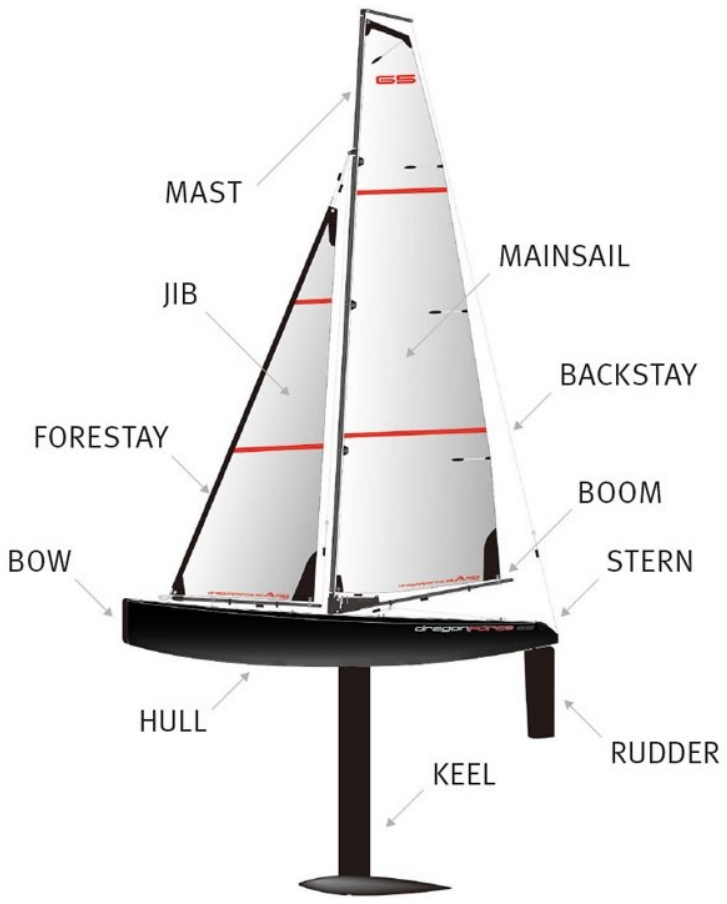
\includegraphics[width = 0.45\textwidth]{figures/sailing/sailboat-parts.png}
\caption{Sailboat parts \cite{sail-parts}}
\label{fig:sail-parts}
\end{wrapfigure}

\section{Sailing Background}
Sailboats work by utilizing the balance of forces created between the sails and the wind as the driving force, the keel/rudder and the sea for controlling the boat, plus the gravity for countering the heel. There are countless online resources to learn about the details of how sailboats work. Here, I will focus on the parts that are important for the project.

\subsection{Basics of Sailing}
Many might think that sailboats move with the wind's pushing on the sail. Although this is true for some wind angles, most of the time the sails work like airplane wings utilizing Bernoulli's Principle. To put it simply, Bernoulli's principle \cite{wiki:bernoulli} states that increasing flow speed in fluids corresponds to decreasing pressure, and vice versa. The shape of the sails resemble an airplane wing. Because of its shape, the air travels faster on one side than the other, which creates a pressure difference, and results in a net force that drives the boat forward. Using the Bernoulli Principle, a sailboat is able to travel in much wider wind angles, compared to what would be possible by using wind push only.

\begin{figure}[h]
\centering
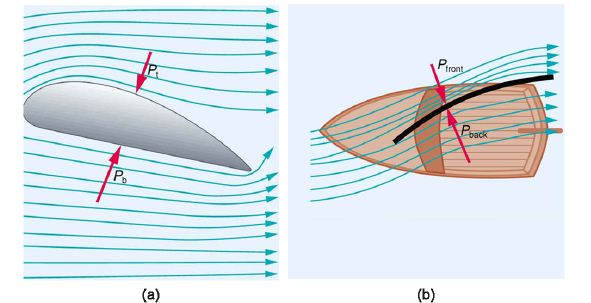
\includegraphics[width = 0.6\hsize]{figures/sailing/sail-bernoulli.jpg}
\caption{Visualization of Bernoulli Principle: (a)Airplane wing, (b)Sail \cite{bernoulli}}
\label{fig:bernoulli}
\end{figure}

\subsection{Point of Sails}
The direction of the boat compared to the wind is called the point of sails. As can be seen in Figure \ref{fig:points-of-sail}, sailboats can go in almost all angles with respect to the wind, except from straight into the wind.

\begin{figure}[h]
\centering
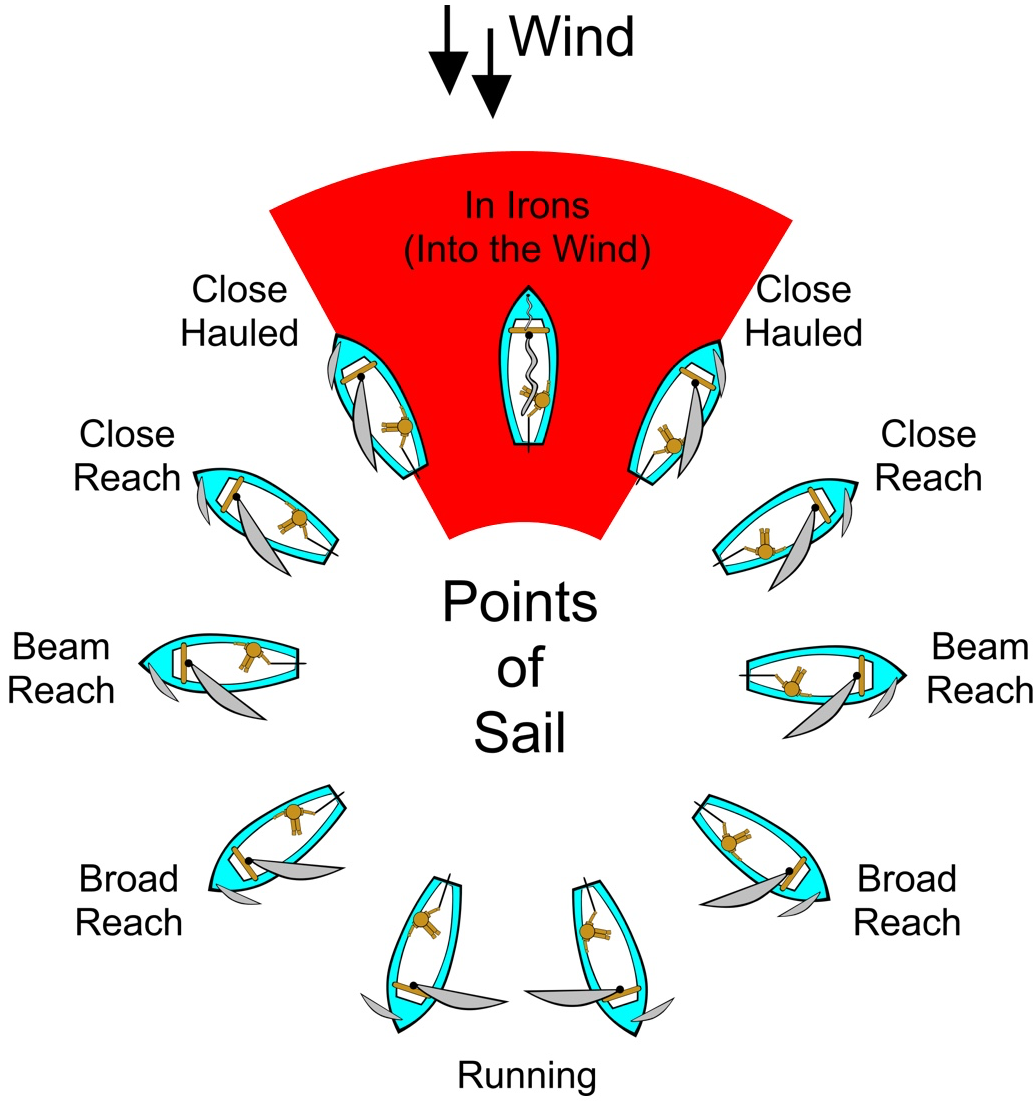
\includegraphics[width = 0.55\hsize]{figures/sailing/PointsOfSail.png}
\caption{Point of Sails \cite{img:sailing-tack-gybe}}
\label{fig:points-of-sail}
\end{figure}

In order to make progress towards the wind, one needs to sail close hauled as seen in Figure \ref{fig:points-of-sail}, and make repeated turns with respect to the wind, known as tack. During a tack, the boat changes direction by turning its head towards and through the wind so that the direction from which the wind blows changes from one side of the boat to the other \cite{wiki:tack}. Jibe is similar to tack, but it is used while sailing downwind, and the boat changes direction by heading away instead of towards the wind. Visualizations of tack and jibe can be seen in Figure \ref{fig:tack-jibe}. 

\begin{figure}[h]
    \centering
    \begin{subfigure}[b]{0.28\textwidth}
        \centering
        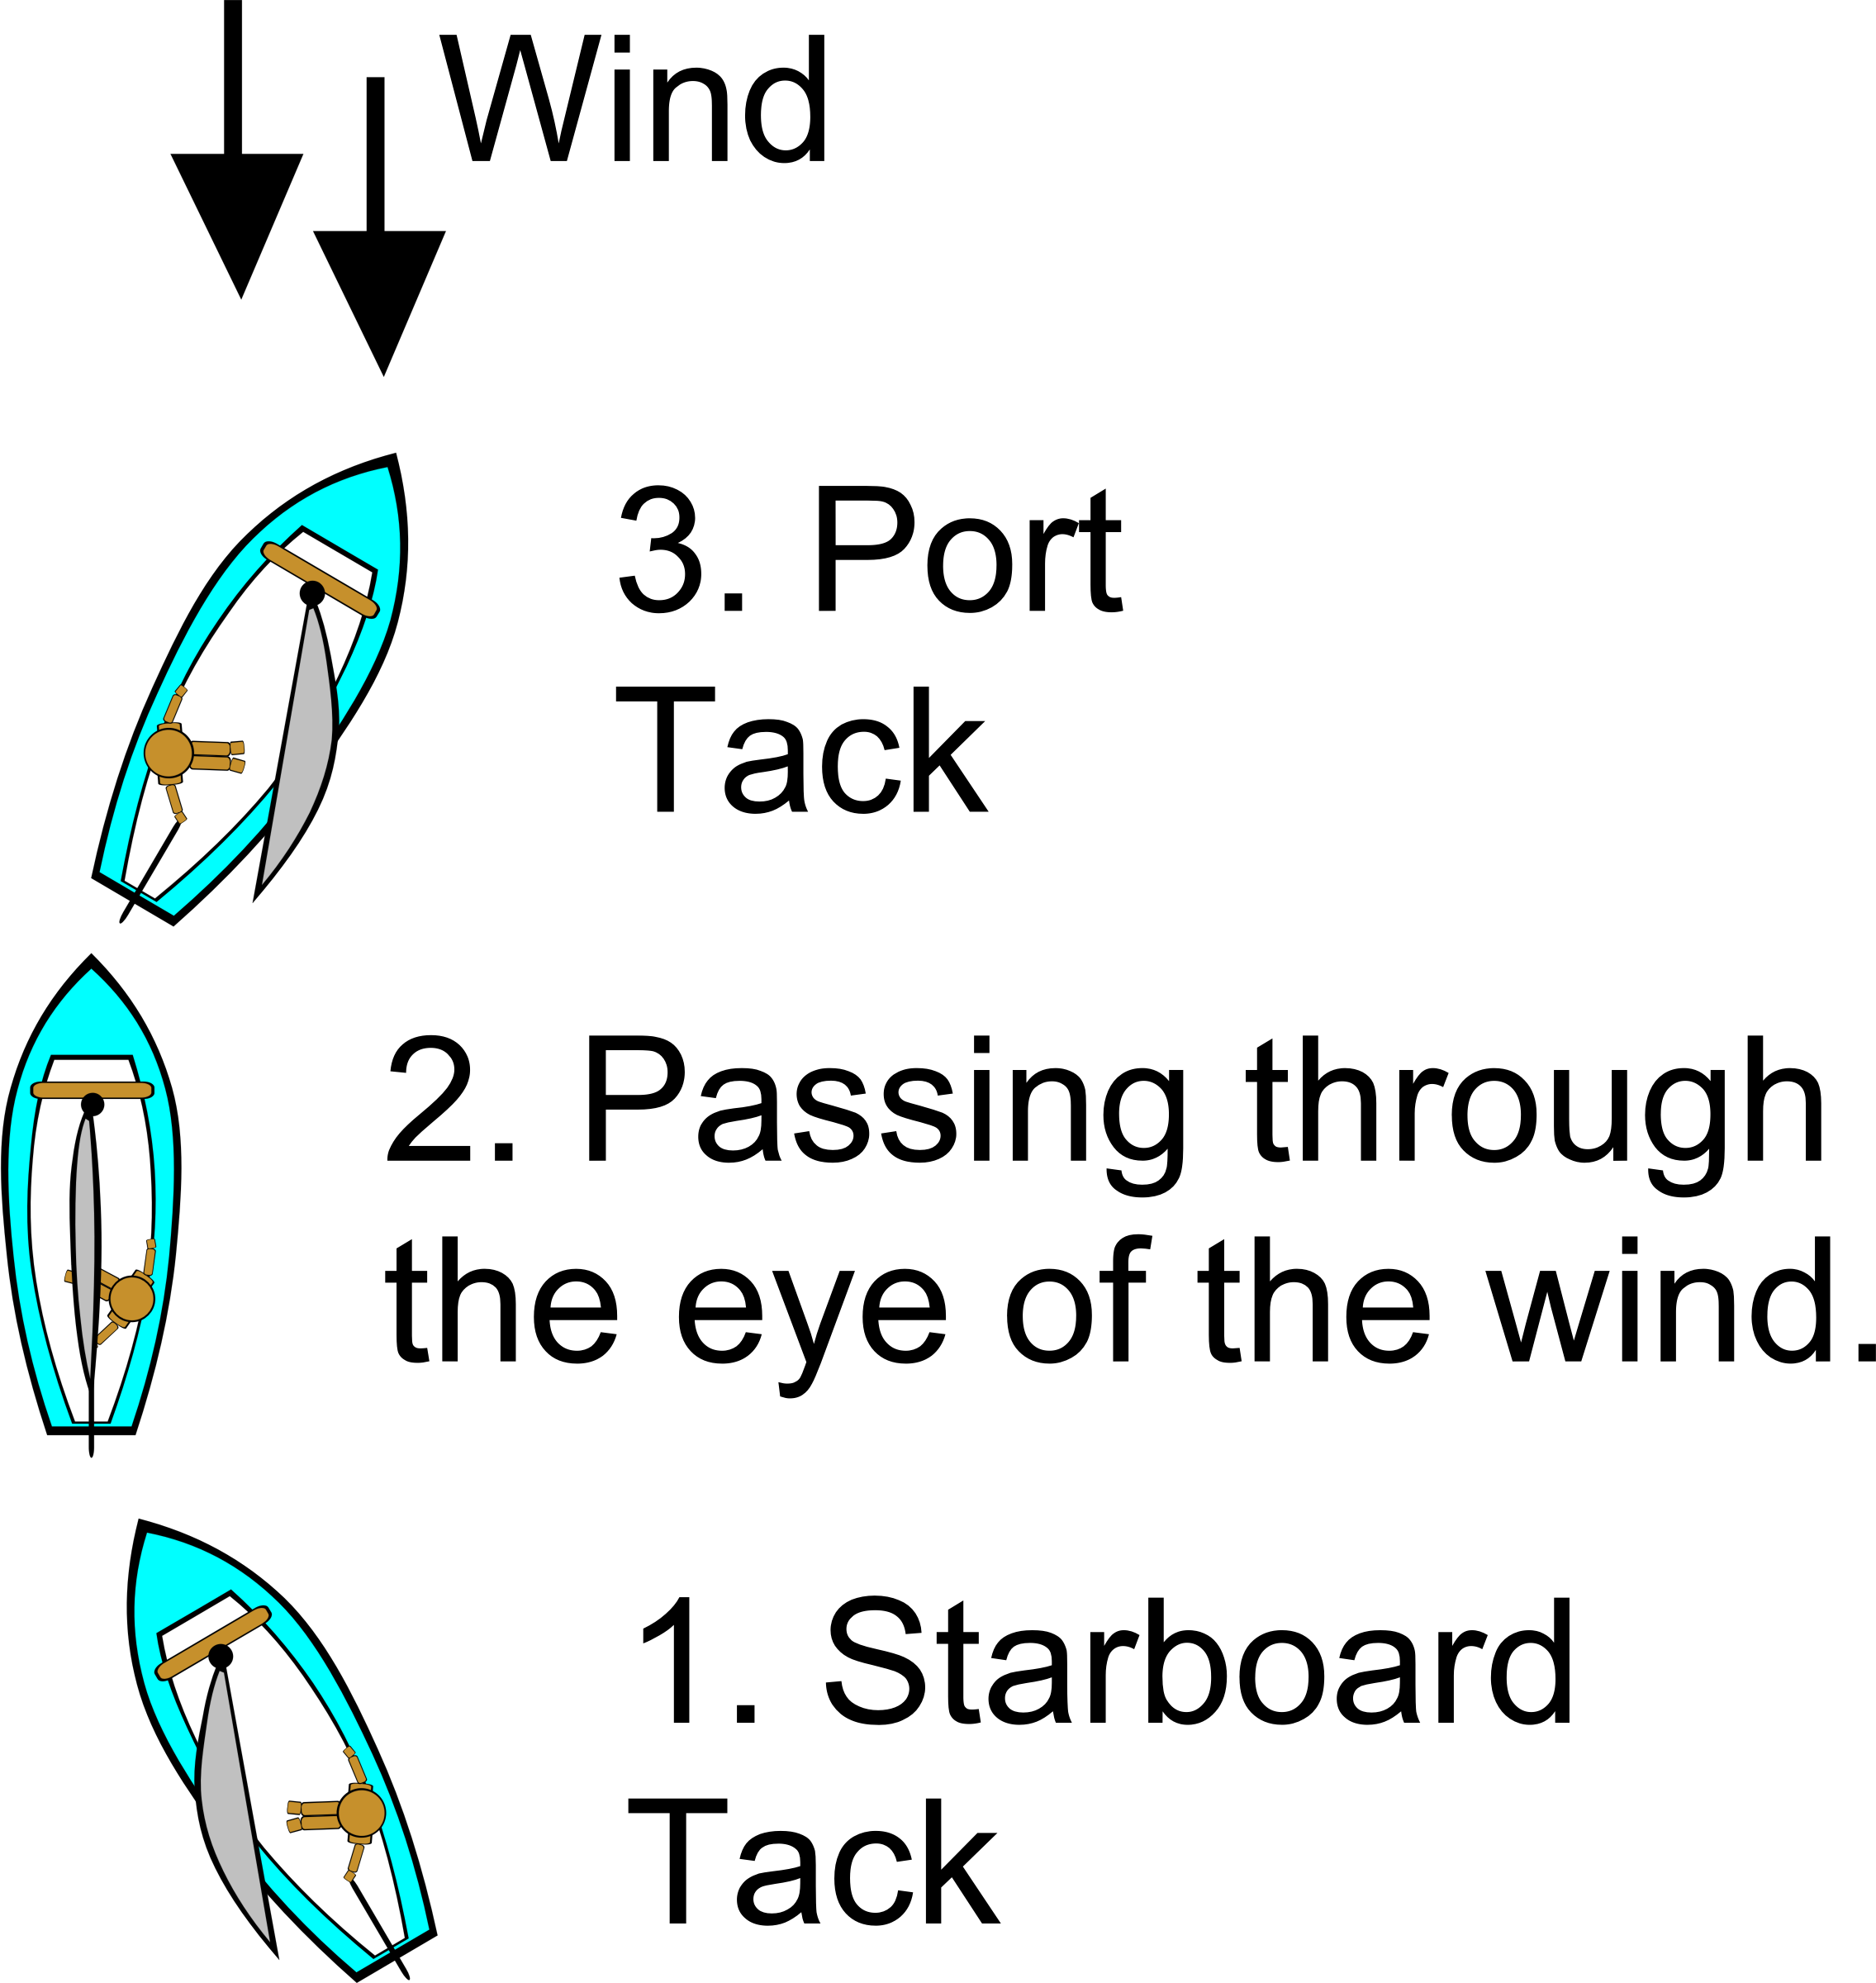
\includegraphics[width=\textwidth]{figures/sailing/tack.png}
        %\caption{tack \cite{img:sailing-tack-gybe}}
        \label{fig:tack}
    \end{subfigure}
    \begin{subfigure}[b]{0.22\textwidth}
        \centering
        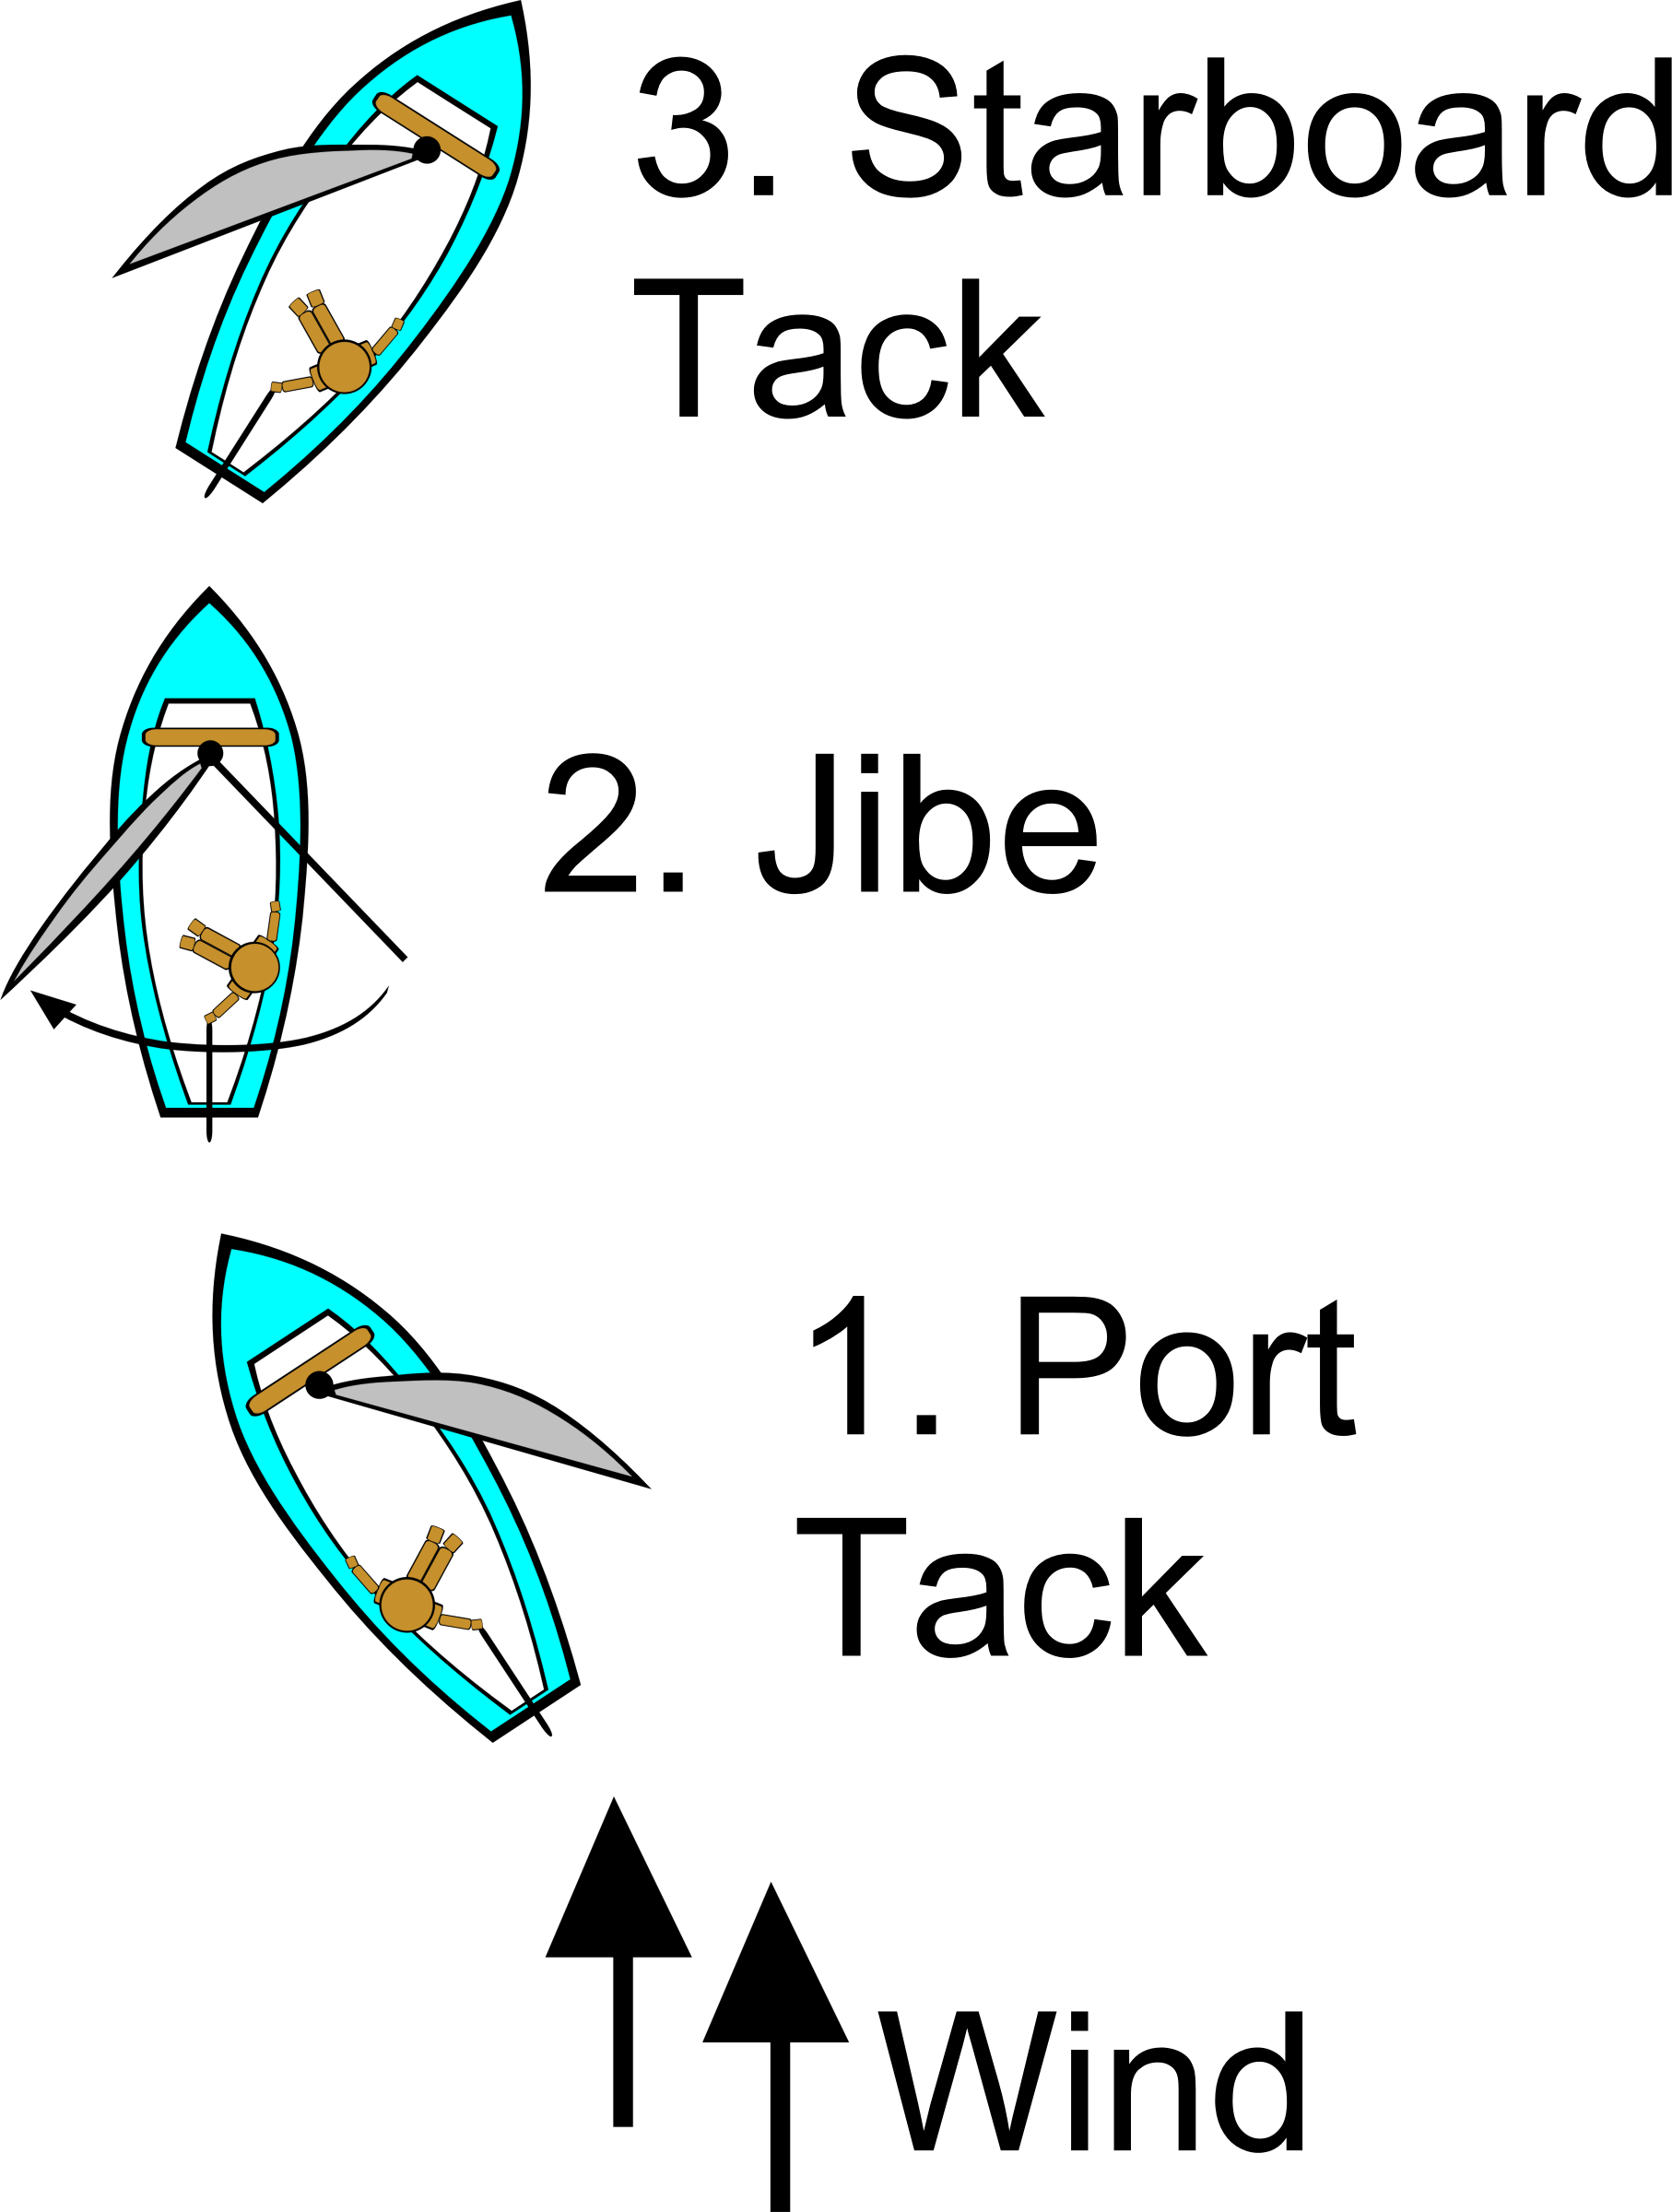
\includegraphics[width=\textwidth]{figures/sailing/jibe.png}
        %\caption{jibe \cite{img:sailing-tack-gybe}}
        \label{fig:jibe}
    \end{subfigure}
    \caption{Tack (left) and Jibe (right) \cite{img:sailing-tack-gybe}}
    \label{fig:tack-jibe}
\end{figure}

Since tacks and jibes require readjustments in sails, an autopilot should not do these manoeuvres unless specifically instructed by the skipper. In addition, the state of the boat differs a lot during tacks and jibes compared straight cruising, which confuses the state estimators we are trying to build. Stanislas \cite{stan} removed tacks from the dataset the models were trained on, and achieved significant performance increase (cf. Section \ref{sec:Stan}).

\subsection{Polar Speed}

Although the boats can sail in many angles with respect to the wind, the optimal angle to sail with is different for each boat due to their unique design. A polar plot, which plots the performance of a boat with reference to the true wind angle, is a helpful tool to judge a boat's optimal angles. The polar plot for Concise 8 can be seen in Figure \ref{fig:polar-plot}. Looking at the polar plot, we can see that the best upwind angle is around 45\degree, whereas the best downwind angle is around 150\degree. In his project, Roman incorporated this optimal degree and speed information in Reinforcement Learning reward \cite{roman}.

\begin{figure}[h]
\centering
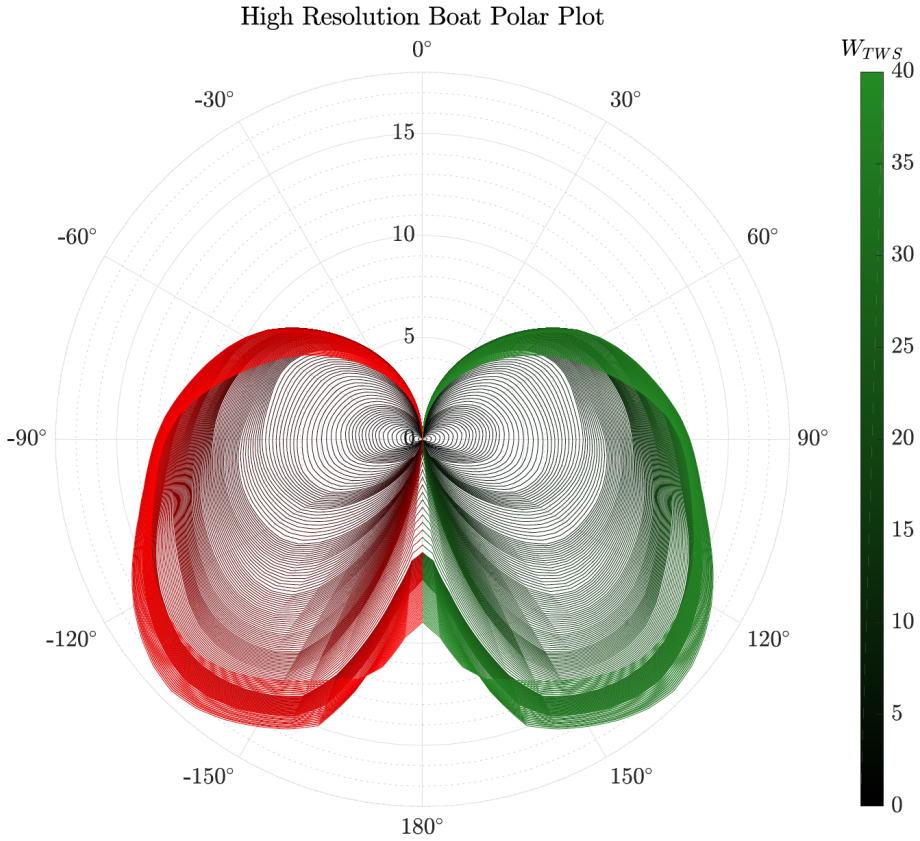
\includegraphics[width = 0.85\hsize]{figures/sailing/polar-plot.png}
\caption{Concise 8 Polar Plot \cite{stan}}
\label{fig:polar-plot}
\end{figure}

\subsection{Elements Affecting Boat Heading}
\subsubsection{Rudder}
The most important element that affects the boat heading is the rudder, whose main purpose is to steer the boat. It works by displacing water at the back of the boat, which creates a force that turns the boat around its center, the keel. Although it is the easiest way to control the boat, moving the rudder creates drag and slows down the boat, so it is not preferable to use it excessively.

\begin{figure}[h]
\centering
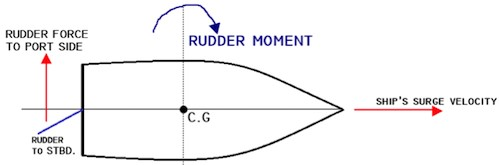
\includegraphics[width = 0.6\textwidth]{figures/sailing/rudder.jpg}
\caption{How rudder works \cite{rudder}}
\label{fig:rudders}
\end{figure}

\subsubsection{Boat Design and Sail Trim}

\begin{wrapfigure}[10]{r}{0.3\textwidth}
\vspace{-1cm}
\centering
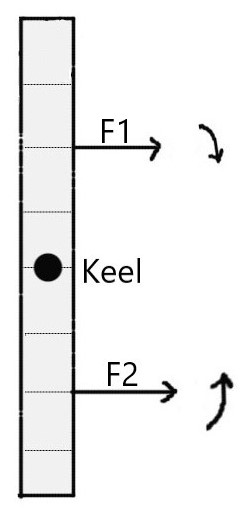
\includegraphics[width = 0.15\textwidth]{figures/sailing/tork.jpg}
\caption{Balance of torque across keel}
\label{fig:keel-tork}
\end{wrapfigure}

If there is more force acting from the front of the keel than from the back of the keel, the boat will naturally turn. This is taken into account when designing the boat, by carefully calculating the area of fore and main sails, position of mast and keel, etc. The balance of these forces can also be altered after the boat is manufactured. For example, many high performance sailing boats have features to adjust the position, angle and bend of the mast. Furthermore, this balance can even be adjusted on the go, by trimming the fore and main sails individually.

\subsubsection{Heel}
Heeling in sailing means the tipping of the sailboat to one side, also known as Roll in boating or aviation. When the boat heels, the boat wants to turn towards the wind. Sailboats heel more as the wind speed increases. This is also factored in during the design of the boat, because continually countering this turn with rudder would significantly slow the boat down.

\begin{figure}[h]
\centering
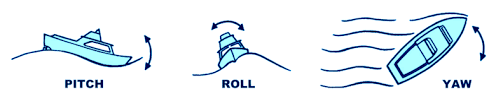
\includegraphics[width = 0.7\textwidth]{figures/sailing/boat-pitch-roll-yaw.png}
\caption{Wave affecting boat \cite{img:pitch-roll-yaw}}
\label{fig:pitch-roll-yaw}
\end{figure}

\subsubsection{Waves}
Waves affect the heading in two ways. First, the momentum of the waves hitting the boat from different angles changes the course of the boat. Second, as the boat moves through the waves, the roll and the pitch of the boat changes, which affects the boat's centre of gravity and how sails interact with wind, resulting in a change in heading.

As we can see, there are a lot of factors that affect the boat heading, and it can't be controlled solely by rudder. This knowledge affected the decisions made in the later parts of the project, for example the Reinforcement Learning environment.


\section{State of the Art Autopilots}

The common consumer autopilots work in a very basic way. It either focuses on the boat's heading, using the data from magnetic compass; or focuses on the apparent wind, using the data from the wind sensor usually found at the top of the mast. The autopilot system compares the current reading and the goal reading, and every time the boat diverges from the goal(e.g., by wind or waves), the autopilot compensates by moving the rudder in the opposite way. 

\begin{figure}[h]
\centering
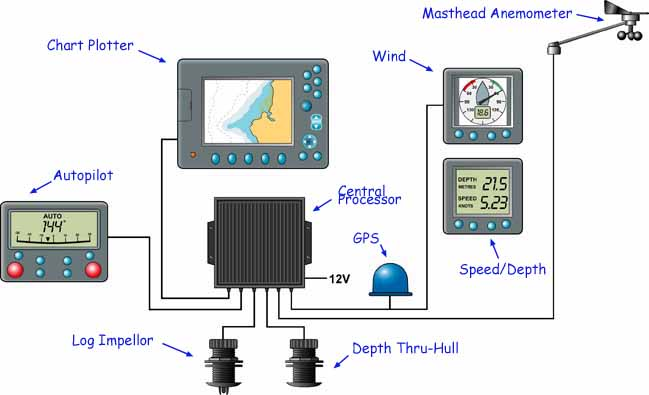
\includegraphics[width = 0.65\textwidth]{figures/other/autopilot.jpg}
\caption{A typical autopilot system \cite{img:autopilot}}
\label{fig:autopilot}
\end{figure}

The focus of common consumer autopilots is to keep the boat on the right course. There are also more advanced options, gaining popularity in the last few years, that focus more on performance and racing. These autopilots have some features that imitates how a professional skipper would steer a boat in certain situations. For example: B\&G autopilots \cite{bandg} have gust response feature that quickly recovers from changes in wind, NKE autopilots \cite{nke} have surf mode that promotes the use of waves in downwind angles \cite{yachting_world_2020}, Raymarine autopilots \cite{raymarine} decide on whether to use apparent or true wind depending on wind angle \cite{cruising_world_2019}.

However, these features are all rule based, usually require manual sensitivity tuning, and does not make use of the recent advancement in computing: machine learning. Madintec is the only company that currently uses machine learning in their autopilots for foiling sailboats \cite{madintec}. Foiling sailboats move at extreme speeds, so getting real-time data does not provide enough time for optimal rudder angle calculation. Madintec utilizes a machine learning model to predict the future boat state, and uses that prediction for autopilot decision making \cite{madintec-eric}.

There are no commercially available autopilots that utilize machine learning any further. One notable attempt to use Reinforcement Learning in Sailboat autopilots was done by the RoboSail project \cite{robosail1}. The authors attempted to make a fully autonomous sailing system based on RL, but concluded that it would need several trips around the world for the algorithm to converge \cite{robosail2}. The Robosail team then took on the prevalent approach of rule based autopilots, but let the RL algorithm decide on the parameters and sensitivities instead \cite{robosail3}.

Thanks to the data from Trigger Racing, plus the work of previous students, T-DAB and Imperial College London employees and supervisors, this project aims to tackle the previously unfulfilled challenge of Reinforcement Learning on real-world sailboat autopilots.

\section{Literature Review: RL Algorithms}
In this section, the modern Reinforcement Learning algorithms and the suggested algorithm to be used for our use case in this project is discussed.

\begin{figure}[h]
\centering
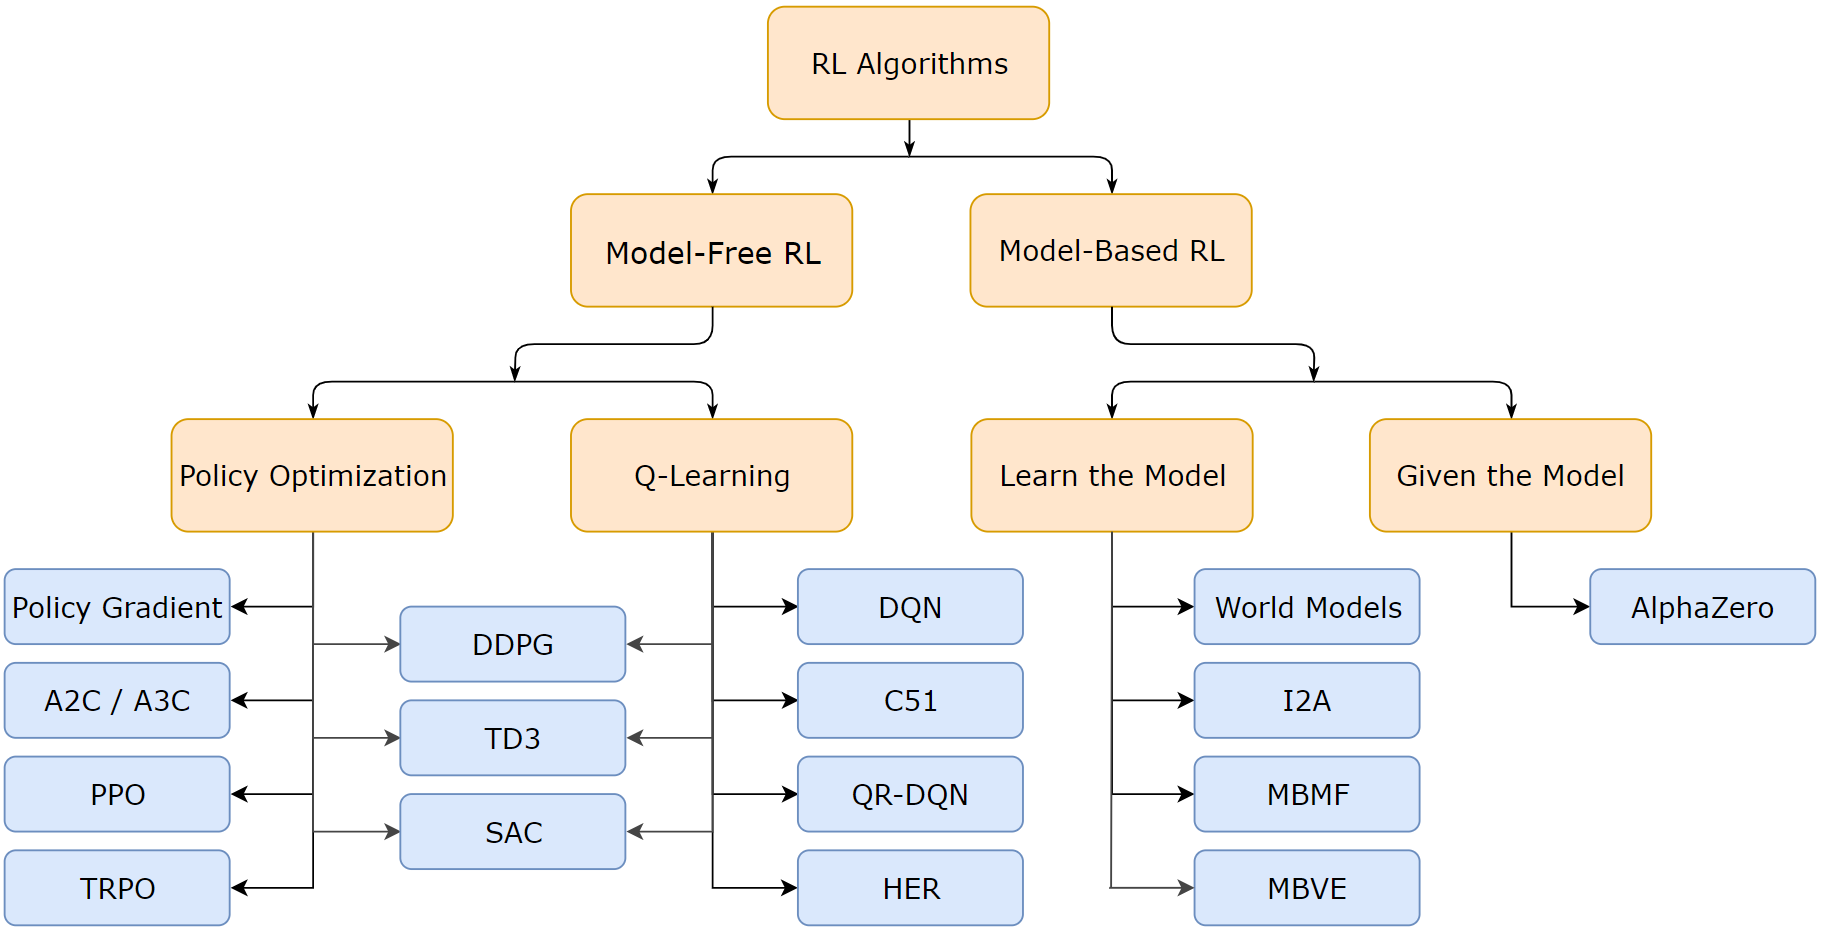
\includegraphics[width = \hsize]{figures/RL algorithms.png}
\caption{A non-exhaustive taxonomy of modern RL algorithms \cite{openai:rl-algs}}
\label{fig:rl-algs}
\end{figure}

An introductory taxonomy of the modern RL algorithms can be seen in Figure ~\ref{fig:rl-algs}. There are two main classes of RL algorithms, Model-Based and Model-Free. In Model-Based algorithms, the algorithms have either access to the environment model, or it learns the environment model. The problem with this branch of algorithms is that usually, the ground truth of the environment is not readily available to the agent. The agent has to learn a simulated environment, then performs poorly on the real environment. This is specifically the case for our project. Furthermore, Model-Based algorithms have not been as extensively developed and tested as the Model-Free algorithms \cite{openai:rl-algs}. Because of these downsides of Model-Based algorithms, I will focus on the Model-Free algorithms for this project.

In Model-Free RL, there are two main techniques: Policy Optimization and Q-Learning. Algorithms such as DDPG, TD3, and SAC - which are state of the are and best suits our use case - uses a hybrid approach of both of these techniques.
DDPG is the first of these algorithms that was developed in 2015, and can be seen as an adaptation of Deep Q-Learning for continuous action spaces \cite{ddpg}. TD3 and SAC were both developed around the same time in 2018. They utilize different tricks to improve DDPG.

\subsection{TD3}
DDPG is prone to overestimating Q-values. Twin Delayed DDPG (TD3) attempts to solve this issue with three tricks: \cite{openai:td3}

\begin{enumerate}
  \item \textbf{Clipped Double-Q Learning:} Instead of one in DDPG, TD3 learns two Q functions, and uses the lesser Q value in the Bellman error loss functions.
  \item \textbf{“Delayed” Policy Updates:} TD3 updates the policy and target networks less frequently than the Q-function. The original paper recommends one policy update for every two Q-function updates.
  \item \textbf{Target Policy Smoothing:} TD3 adds noise to the target action, to make it harder for the policy to exploit Q-function errors by smoothing out Q along changes in action.
\end{enumerate}

\begin{figure}[h]
\centering
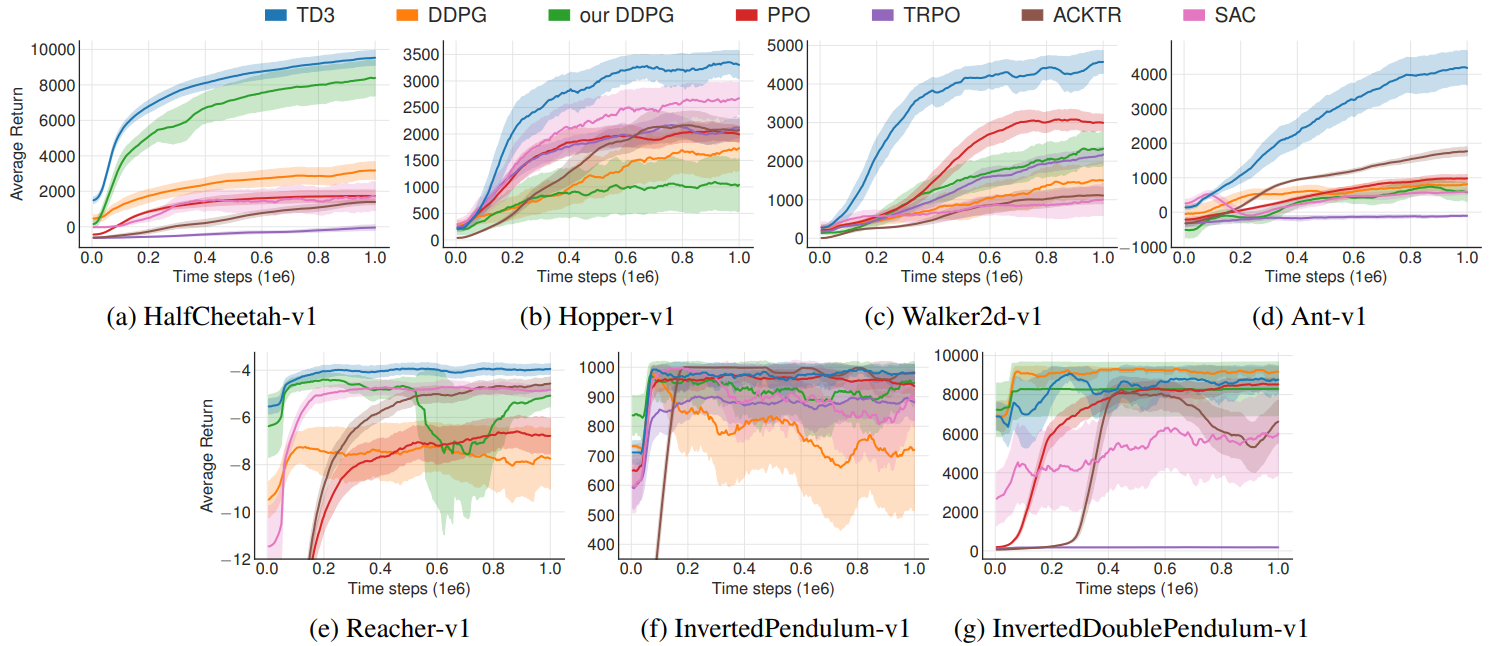
\includegraphics[width = \hsize]{figures/td3 comparison.png}
\caption{Performance comparison of RL algorithms in TD3 paper \cite{td3}}
\label{fig:td3-comparisons}
\end{figure}

In the original TD3 paper, Fujimoto et al. claims that TD3 outperforms the state of the art in every OpenAI gym task tested \cite{td3}. The comparison of the algorithms in different environments can be seen in Figure~\ref{fig:td3-comparisons}.

\subsection{SAC}
Instead of deterministic policies used in DDPG and TD3, SAC uses stochastic policies. Thus, it is a bridge between stochastic policy optimization and DDPG-style approaches. Like TD3, it uses a few tricks to improve DDPG: \cite{openai:sac}

\begin{enumerate}
  \item \textbf{Entropy Regularization:} The policy is trained to maximize a trade-off between expected return and entropy. This is closely related to exploration-exploitation trade-off: higher entropy results in more exploration, which can accelerate learning and prevent converging to bad local optimum.
  \item \textbf{Next-State Actions:} In SAC, the next-state actions used in the target come from the current policy instead of the target policy.
  \item \textbf{Clipped Double-Q Learning:} Like TD3, SAC makes use of Clipped Double-Q Learning.
  \item \textbf{Target Policy Smoothing:} Although there is no explicit target policy smoothing, since SAC uses a stochastic policy, the noise from the randomness achieves a similar effect.
\end{enumerate}

\begin{figure}[h]
\centering
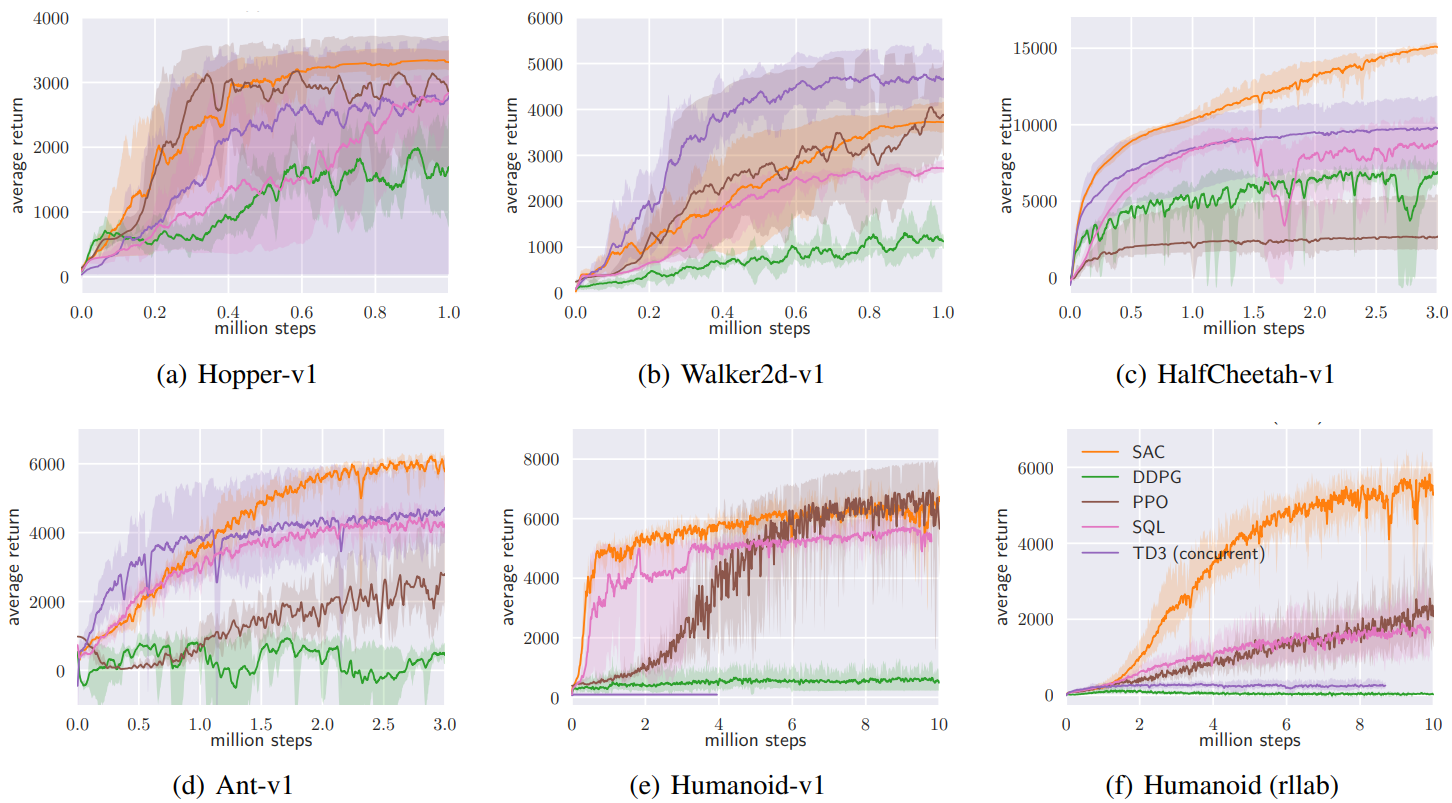
\includegraphics[width = \hsize]{figures/sac comparison og.png}
\caption{Performance comparison of RL algorithms in SAC paper \cite{sacOG}}
\label{fig:sac-comparisons}
\end{figure}

In the original SAC paper, Haarnoja et al. claims that SAC outperforms the state of the art algorithms in sample-efficiency, asymptotic performance, and stability \cite{sacOG}. The comparison of the algorithms in different environments can be seen in Figure~\ref{fig:sac-comparisons}.

\subsection{Algorithm of Choice}
Interestingly, both SAC and TD3 authors claim that they perform better than each other in their own papers. So a third party benchmark is necessary to be able to compare the two algorithms. A comparison of OpenAI PyTorch implementations of TD3, SAC, and few other algorithms can be seen in Figure \ref{fig:openAI-comparisons}.

\begin{figure}[h]
     \centering
     \begin{subfigure}[b]{0.4\textwidth}
         \centering
         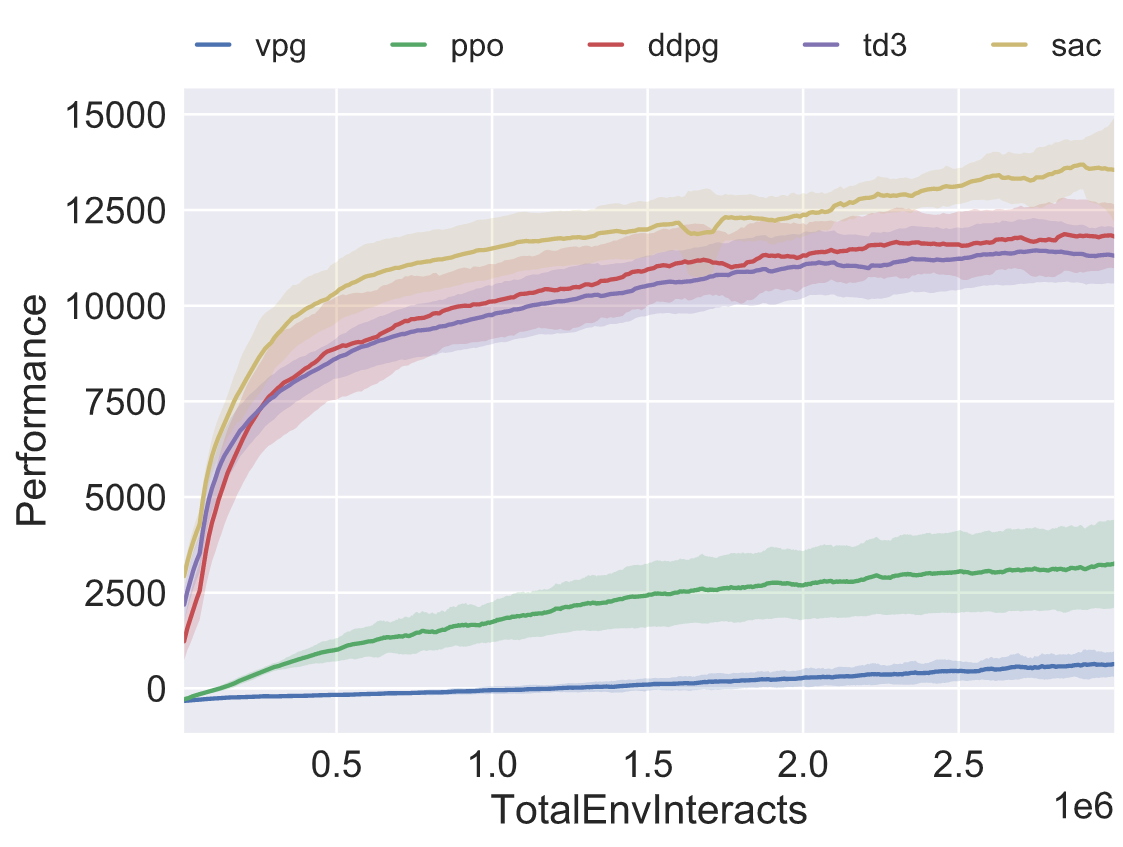
\includegraphics[width=\textwidth]{figures/OpenAI benchmarks/halfcheetah pt.png}
         \caption{HalfCheetah-v3}
     \end{subfigure}
     \quad
     \begin{subfigure}[b]{0.4\textwidth}
         \centering
         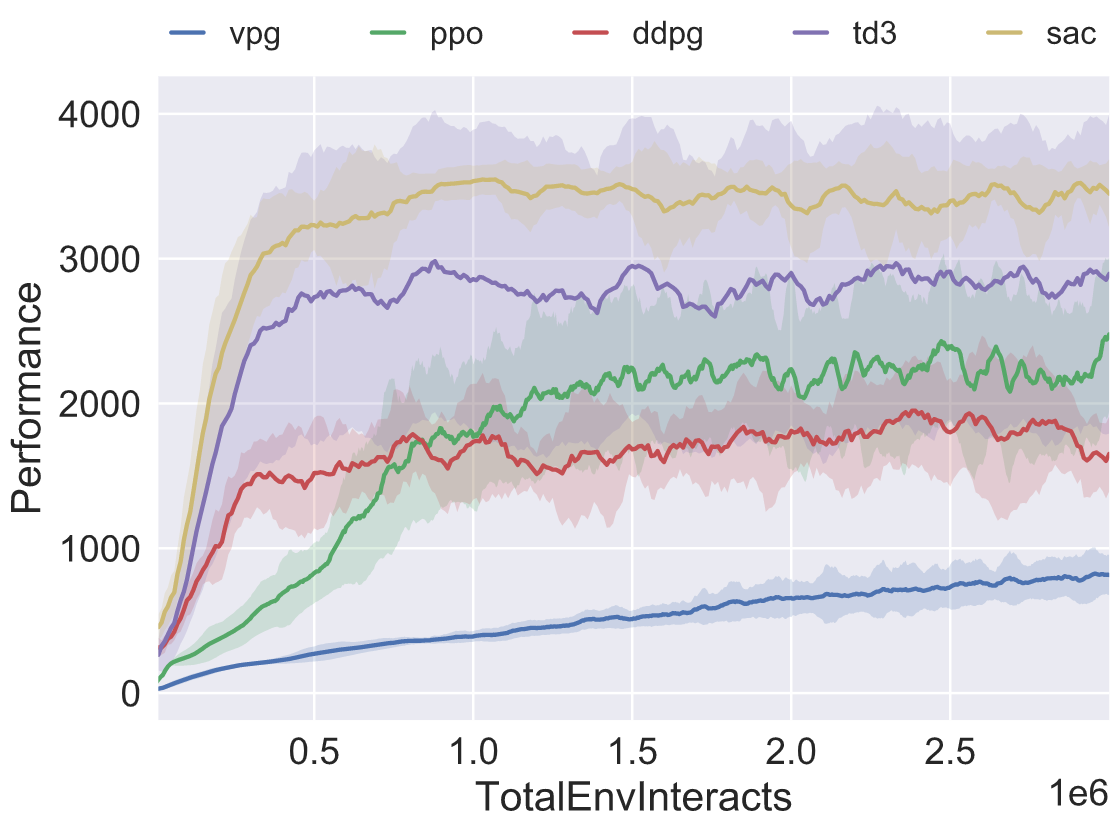
\includegraphics[width=\textwidth]{figures/OpenAI benchmarks/hopper pt.png}
         \caption{Hopper-v3}
     \end{subfigure}
     \quad
     \begin{subfigure}[b]{0.4\textwidth}
         \centering
         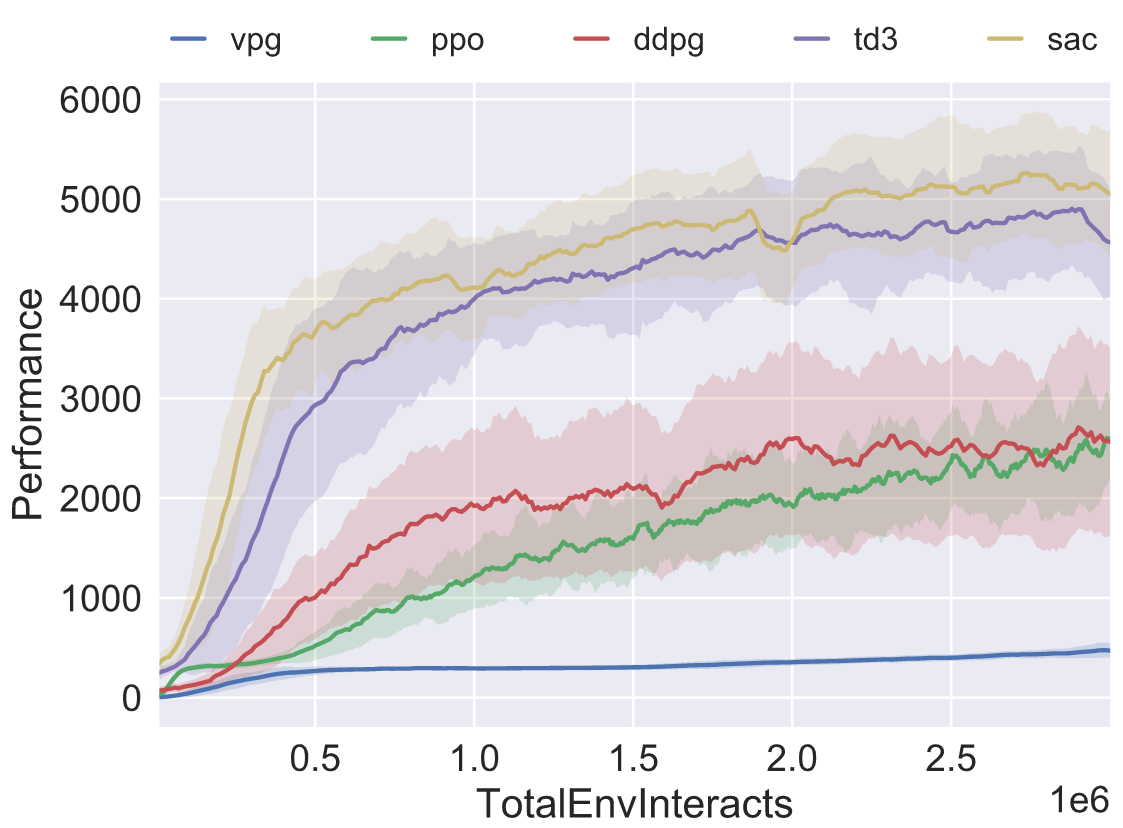
\includegraphics[width=\textwidth]{figures/OpenAI benchmarks/walker pt.png}
         \caption{Walker2d-v3}
     \end{subfigure}
     \quad
     \begin{subfigure}[b]{0.4\textwidth}
         \centering
         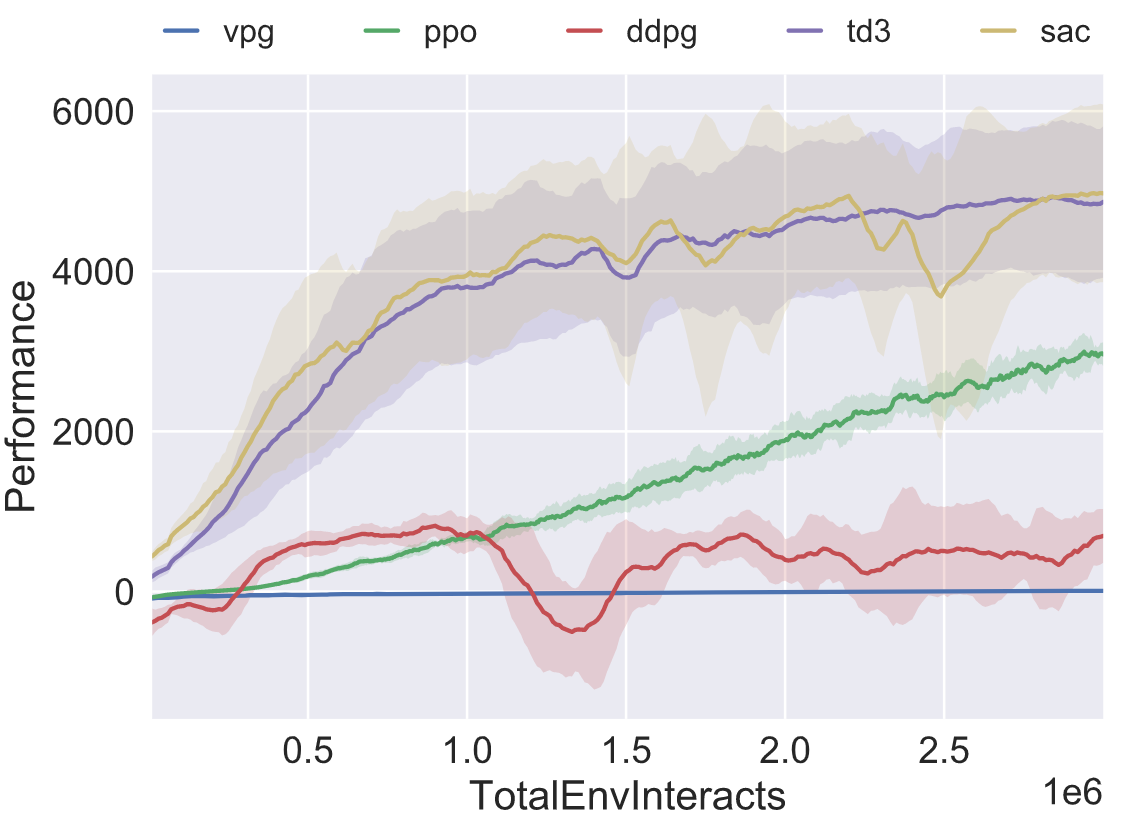
\includegraphics[width=\textwidth]{figures/OpenAI benchmarks/ant pt.png}
         \caption{Ant-v3}
     \end{subfigure}
        \caption{Performance comparison of OpenAI implementations of RL algorithms \cite{openai:bench}}
        \label{fig:openAI-comparisons}
\end{figure}

As can be seen in Figure \ref{fig:openAI-comparisons}, TD3 and SAC perform closely to each other, with SAC having a slight advantage over TD3. However one should note that OpenAI implementation of SAC have slight variations that bring it closer to TD3 \cite{openai:sac-code}.

The advantage of TD3 is that it performs really close to SAC, with less complexity and less hyperparameters to tune. However, the second iteration of SAC from the original authors automatically tunes the problematic temperature hyperparameter, reducing the problem of hyperparameter tuning, making the algorithm more stable among different seeds and environments, and performs well even in the worst case, which is important for real life use cases \cite{sacOG}. 

Because of these reasons, the suggested algorithm to be used for the Reinforcement Learning Approach is Soft Actor-Critic (SAC).

\subsection{Recent Advancement: Truncated Quantile Critics}

Truncated Quantile Critics (TQC) is a novel algorithm whose original paper was published in May 2020 \cite{tqc-paper}. TQC aims to solve the overestimation bias in continuous off-policy learning by combining three ideas: distributional representation of a critic, truncation of critics prediction, and ensembling of multiple critics. The authors claim that TQC outperforms the current state of the art in all the environments they tested. The comparison of the algorithms can be seen in Figure \ref{fig:tqc-comparison}.

\begin{figure}[h]
\centering
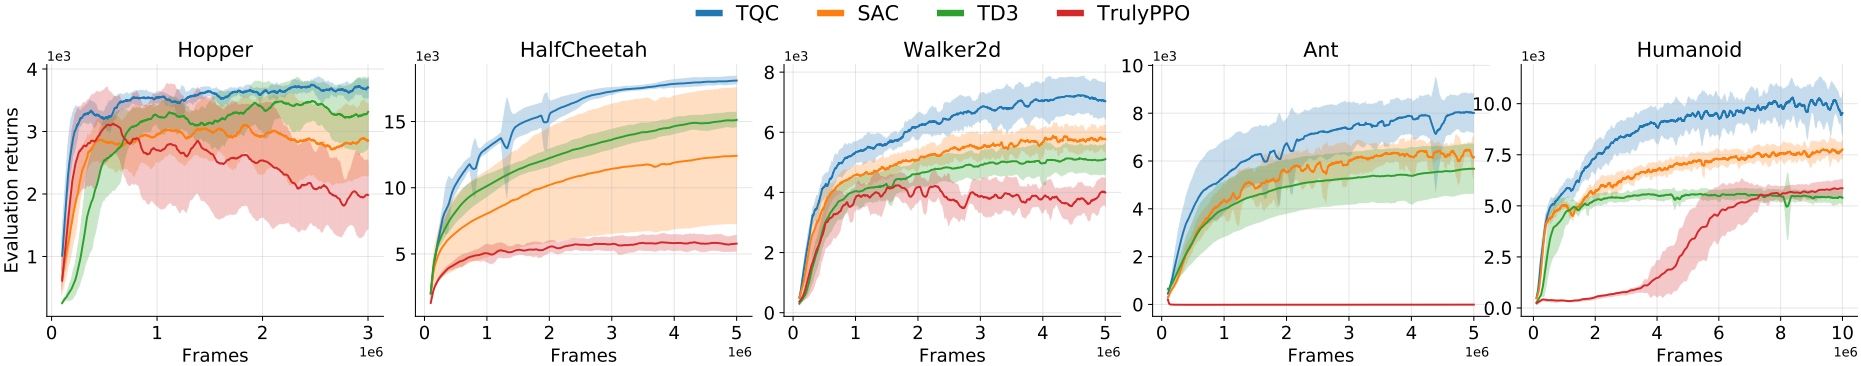
\includegraphics[width = \hsize]{figures/tqc comparison.png}
\caption{Average performance of RL algorithms on MuJoCo Gym Environments \cite{tqc-paper}}
\label{fig:tqc-comparison}
\end{figure}

TQC is not as thoroughly tested as the current state of the art, but it shows promising results, especially in the harder environments. Although it is in beta, there is an implementation of TQC publicly available. Therefore, this new advancement in continuous RL algorithms will definitely be incorporated in this project.

\section{Literature Review: Sim2Real RL}
The challenge of trying to solve a real world problem by training on simulated data like we are dealing with in this project is known as Sim2Real. A nice example of these Sim2Real challenges is AWS DeepRacer \cite{aws-deepracer}.

\begin{figure}[h]
     \centering
     \begin{subfigure}[b]{0.49\textwidth}
         \centering
         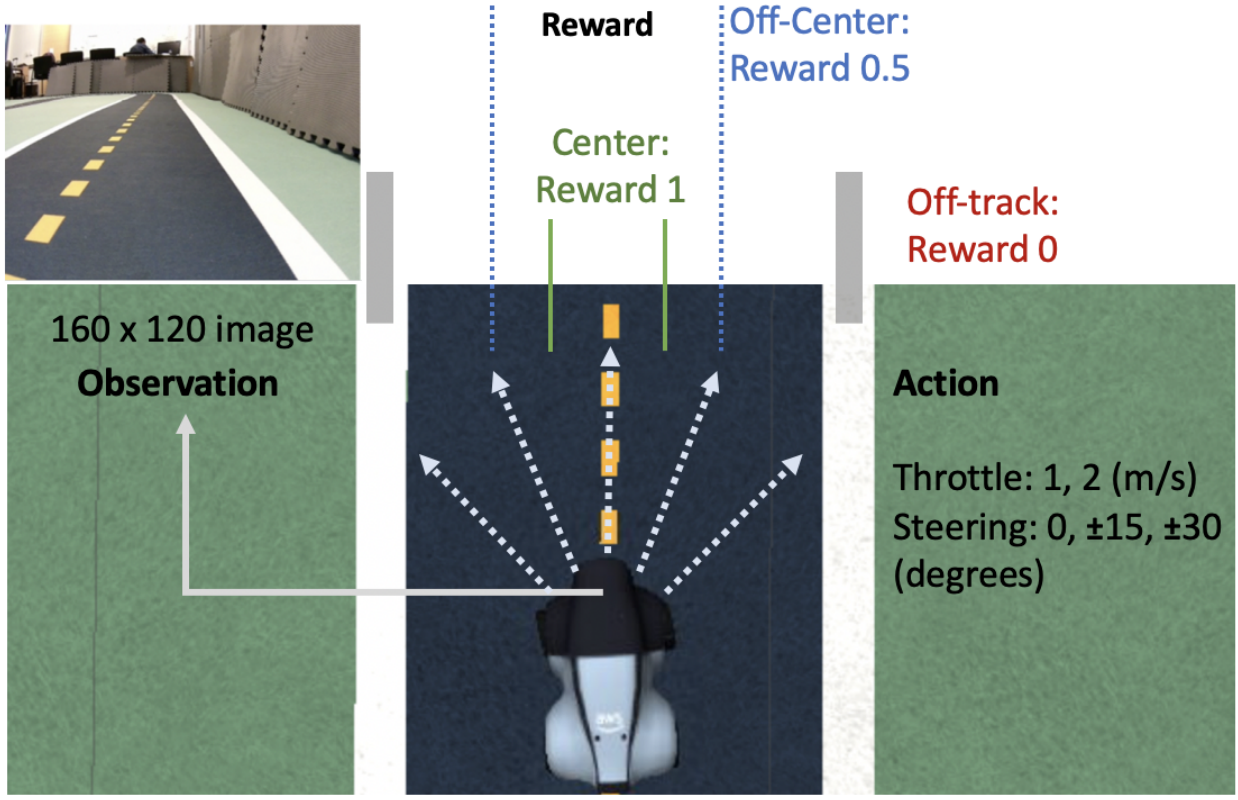
\includegraphics[width=\textwidth]{figures/other/deepracer-obs-act-rew.png}
         \caption{Observation, action and reward for DeepRacer agent}
     \end{subfigure}
     \hfill
     \begin{subfigure}[b]{0.49\textwidth}
         \centering
         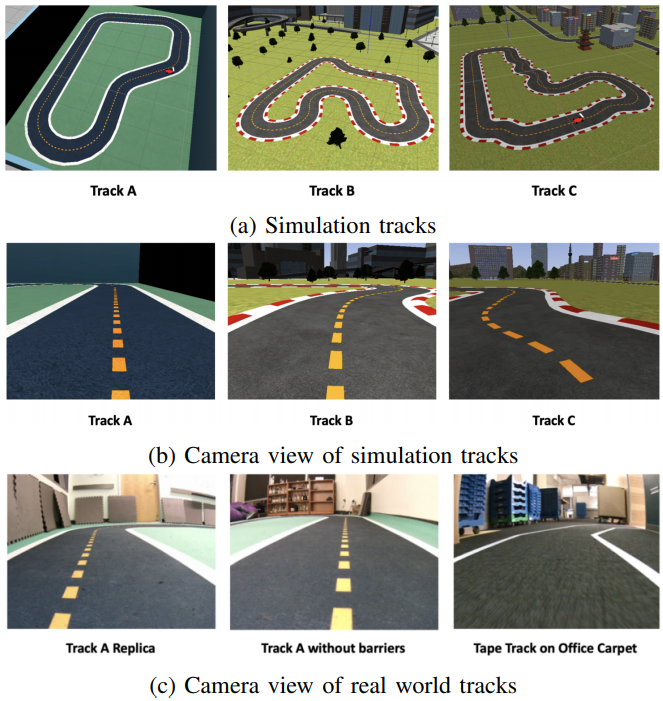
\includegraphics[width=0.9\textwidth]{figures/other/deepracer-tracks.png}
         %\caption{Stable Baselines3 implementation (Tuned parameters) - Goal Achieved in 200.000 steps}
     \end{subfigure}
        \caption{AWS DeepRacer \cite{aws-deepracer}}
        \label{fig:aws-deepracer}
\end{figure}

AWS DeepRacer is a global open competition where everyone can train their RL Agents on a 3D Racing simulator and compete with them online. The highest ranking competitors are then invited to the Championship Cup, where they compete with their agents on a race with a physical 1/18 scale race car.

This \textit{Automation and Intelligent Optimisation in High Performance Sailing Boats} project aims for a similar goal on boats instead of cars. We are trying to train an autopilot with Reinforcement Learning on a simulation based on the state estimator models. If the RL Agent shows satisfactory performance, it can then be translated onto real world boats and use real sensor data instead of simulated boat sensors data.

The RL Agent setup of this project is similar to that of the AWS DeepRacer shown in Figure \ref{fig:aws-deepracer}, but adapted to a boat setting. The observation of the Agent is not an image, but the sensors in the boat. The action the Agent takes is setting the rudder angle instead of throttle and steering of the car, and the reward is calculated with respect to the goal waypoint. The details of the Reinforcement Learning setting can be seen in \ref{sec:gym-environment} - \nameref{sec:gym-environment} Section.


\section{Previous Work}
The "Automation and Intelligent Optimisation in High Performance Sailing Boats" project started in 2019. Birk Ulstad and Roman Kastusik started working on the project simultaneously. Birk Ulstad took the Supervised Learning Approach, whereas Roman Kastusik took the Reinforcement Learning Approach to the problem. Following their work, Stanislas Hannabelle continued working on the supervised learning approach in late 2019. In 2020, Charles Metz continued the Reinforcement Learning work of Roman Kastusik. Finally, Thomas Ryder continued Charles work before I picked up the project. A very brief summary of everyone's work is presented below.
%I, Doruk Taneli, will be picking up where Birk, Roman, Stanislas, and Charles left off and  further improve the project.

\subsection{Birk Ulstad}
Birk's goal was to develop a supervised machine learning model that predicts the rudder angle set by Jack Trigger on the Concise 8 boat, using the previous data recorded during races by the existing sensors on the boat \cite{birk}.

Birk Ulstad converted the available raw, partially corrupted data to processable csv data. He then cleaned the csv data by removing the irrelevant and corrupted parts, analysing outliers and applying smoothing. Next, he normalized, reframed, and downsampled the data to get it ready for the supervised learning model.

\begin{figure}[h]
\centering
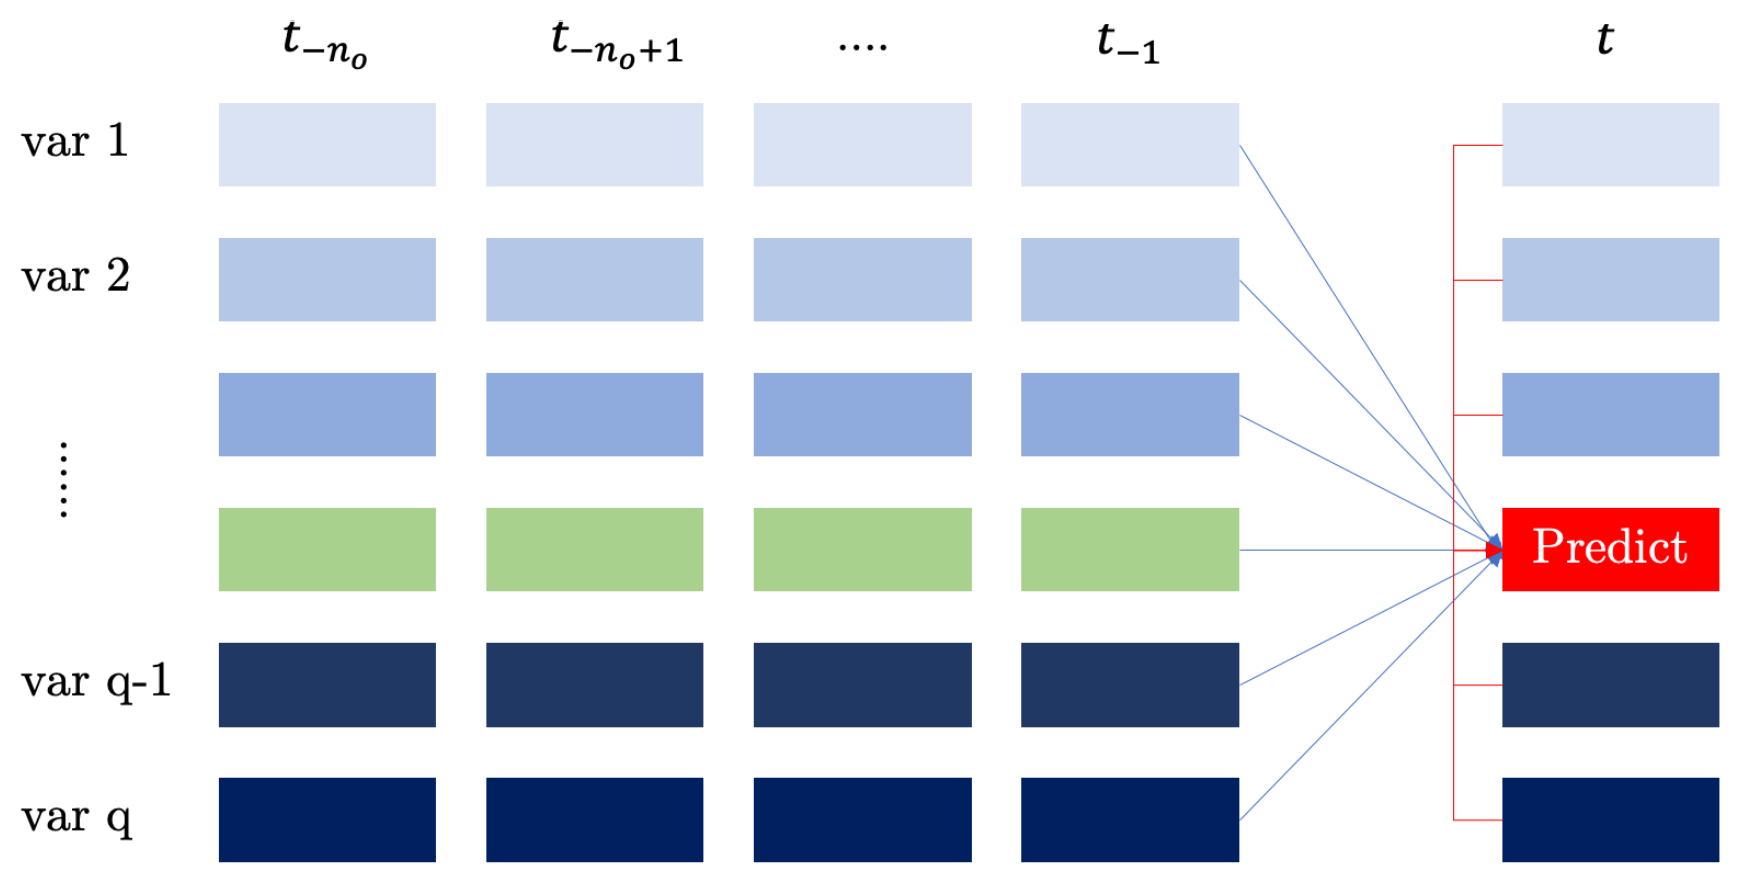
\includegraphics[width = 0.7\hsize]{figures/Birk Ulstad LSTM prediction.png}
\caption{Birk Ulstad's LSTM prediction methods \cite{birk}}
\label{fig:birk lstm}
\end{figure}

For the model, Birk preferred a two stateful LSTM layers, each followed by a dropout layer to prevent overfitting. The prediction plan of the model can be seen in Figure~\ref{fig:birk lstm}. The original plan was to use both past values of the feature set until time t-1 (blue arrows) and the current values at time t (red arrows) to predict the rudder angle. However he only managed to get blue arrow predictions to work, and used those while discussing his results.

Birk concluded that his model architecture is able to predict the rudder angle produced by a human within a couple of degrees. His other notable observations were: 
\begin{itemize}
  \item The model is able to predict the autopilot's rudder angle with much less error compared to a human's rudder angle. Birk explained this as "Learning a univariate rule-based function [of an autopilot] is easier than learning the multivariate function that maps human sensory input to human rudder output".
  \item Downsampling the available data to 5 Hz from 25 Hz is a good middle ground between training time and RMSE. 
  \item An input sequence length between 5-15 seconds provides an optimal trade-off between training time and prediction accuracy.
\end{itemize} 

\subsection{Roman Kastusik}
Roman's objective was to utilize reinforcement learning to increase the autopilots' performance, potentially beyond human level. To achieve this, he trained an LSTM state estimator to simulate the boat's behavior using Jack Trigger's race data, and created a reinforcement learning algorithm that would interact with said simulation environment \cite{roman}.

Roman started with some data analysis, data cleaning, and scaling on Jack Trigger's race data. He then used this data to train the simulation environment that would be used for the reinforcement learning algorithm. The data flow around the simulation environment and the reinforcement learning algorithm can be found in Figure \ref{fig:roman dataflow}.

\begin{figure}[h]
\centering
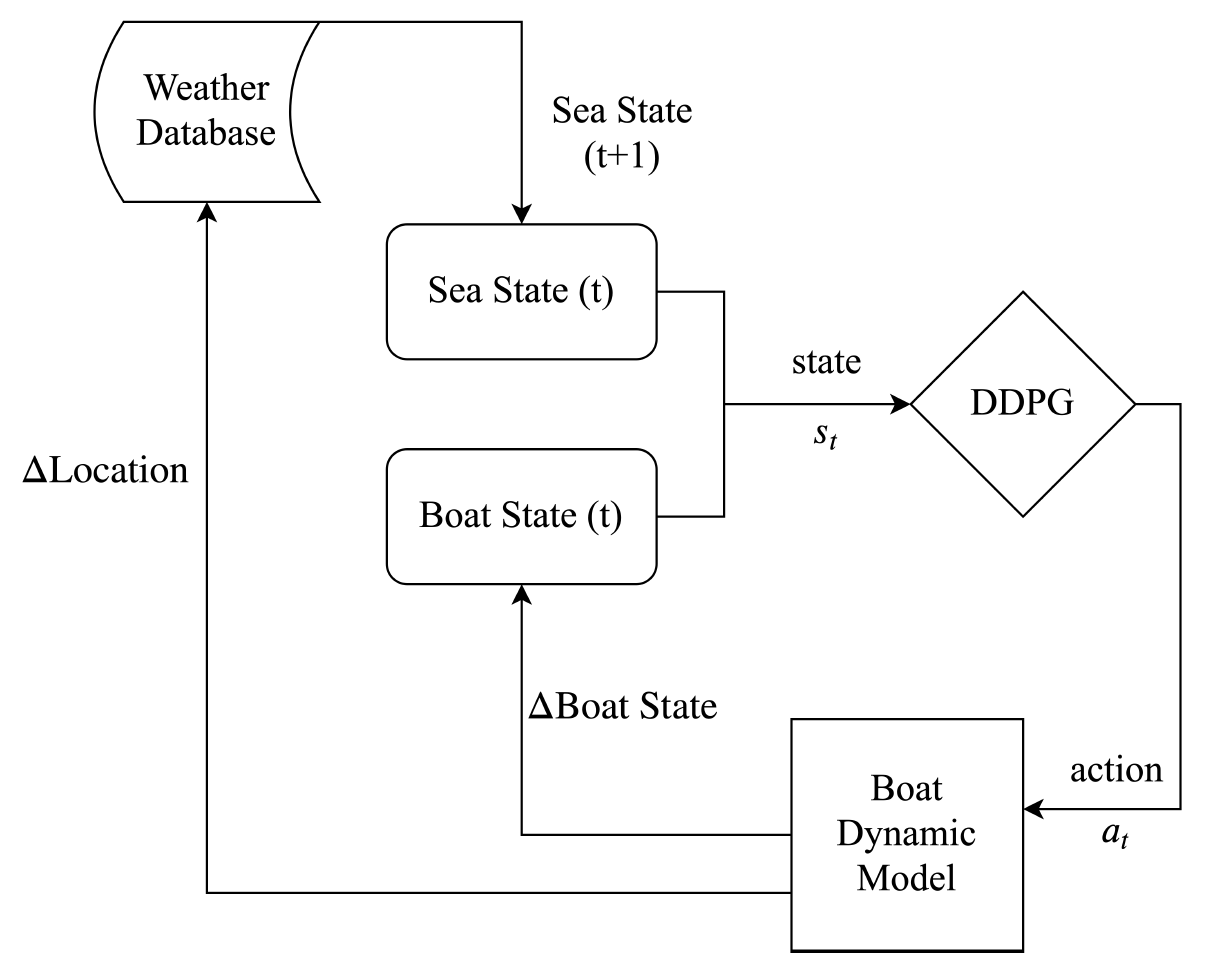
\includegraphics[width = 0.7\textwidth]{figures/roman data flow.png}
\caption{Roman Kastusik's RL data flow \cite{roman}}
\label{fig:roman dataflow}
\end{figure}

He also did research about the recent advancements in reinforcement learning, and created an RL algorithm utilizing Deep Deterministic Policy Gradients, Actor-Critic Networks and Experience Replay.

Roman concluded that due to the poor performance of the simulation environment, it was not possible to realize the full potential of the reinforcement learning algorithm. Charles Metz later continues his work and improves the simulation environment.

\subsection{Stanislas Hannabelle} \label{sec:Stan}
Stanislas' goal was to improve the results of Birk Ulstad's supervised learning approach to the problem. He further cleaned the dataset using a tack\footnote{Tacking is a sailing maneuver where the boat changes direction by turning its head towards and through the wind so that the direction from which the wind blows changes from one side of the boat to the other, allowing progress in the desired direction \cite{wiki:tack}.} detection system, did hyperparameter and bayesian optimization, and compared GRU and LSTM models. He was able to reduce the Root Mean Squared Error from 3.493 degrees of Birk's final model to 1.096 degrees, and reduced the computational time needed for rudder angle prediction \cite{stan}.

\begin{figure}[h]
\centering
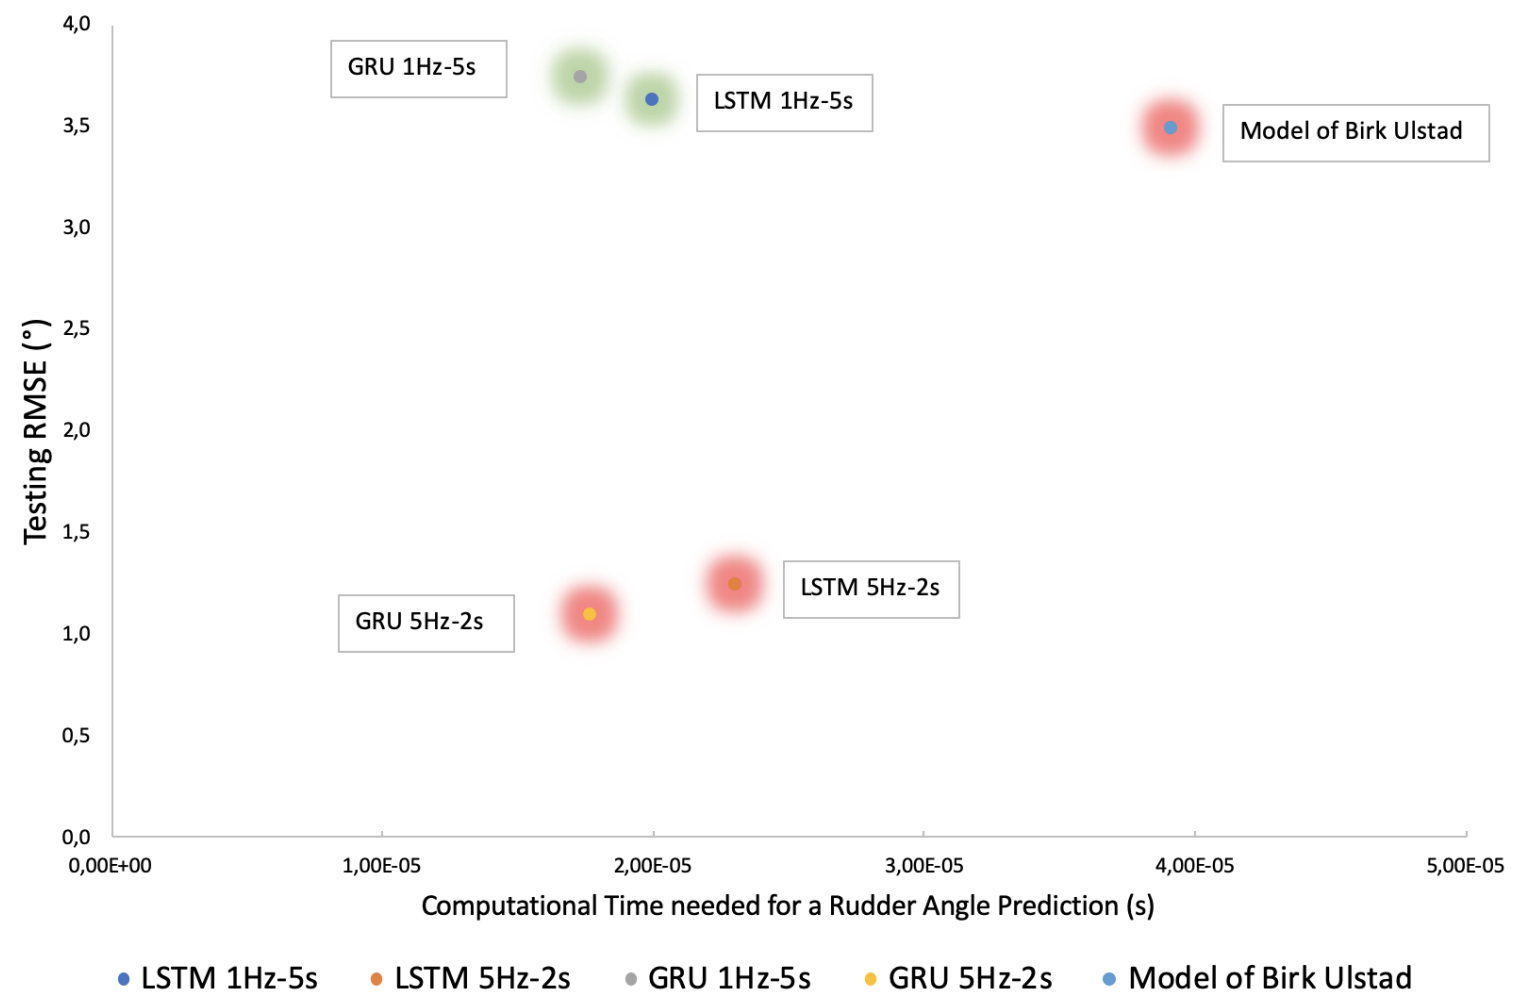
\includegraphics[width = 0.9\hsize]{figures/stan results.png}
\caption{Stanislas Hannabelle's improvements on supervised learning approach \cite{stan}}
\label{fig:stan results}
\end{figure}

Stanislas further cleaned the available dataset by training a classifier to remove tacks, and manually removing the abnormal sailing conditions such as extremely light wind. With the new dataset, he performed the grid search shown in Table \ref{tbl:stan grid} for best sampling frequency (Hz) and input sequence length (seconds). He then performed bayesian optimization for LSTM and GRU models for 1Hz-5s and 5hz-2s parameters. After training and testing with the best hyperparameters he found, Stanislas got the results in Figure \ref{fig:stan results}.

\begin{table}[h]
\centering
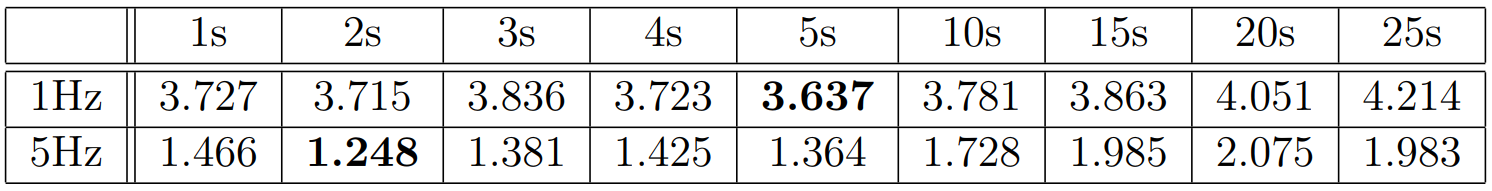
\includegraphics[width=\linewidth]{figures/stan grid search.png}
\caption{validation RMSE for sampling frequency and input length combinations \cite{stan}}
\label{tbl:stan grid}
\end{table}

With his best model 'GRU 5Hz-2s', Stanislas reduced the testing RMSE of Birk's model by approximately 68\% while cutting the required training time in half. Stanislas' model was able to predict the rudder angle produced by a human by around 1 degree. His other success was to reduce the computational time needed for rudder angle prediction so that the model can be implemented live in onboard autopilots.

\subsection{Charles Metz}
Charles' goal was to improve the state estimator model Roman suggested, so it can reliably reproduce the behaviour of a sailing boat in its sea environment. His main idea was that instead of using 1 model to predict \emph{n} sea and boat features like Roman, he used \emph{n} models to predict \emph{n} different features, which lead to very significant improvement \cite{charles}.

Charles had a new dataset available, so he started by applying similar cleaning and preprocessing steps to this new dataset. He noticed that some of the features can be derived mathematically from other features such as true wind, apparent wind, and boat speed. He decided to calculate those features mathematically, then trained \emph{n} separate models for \emph{n} remaining features. He tried 2 different models, model 1 has two final dense layers whereas model 2 has only one final dense layer.

\begin{table}[h]
\centering
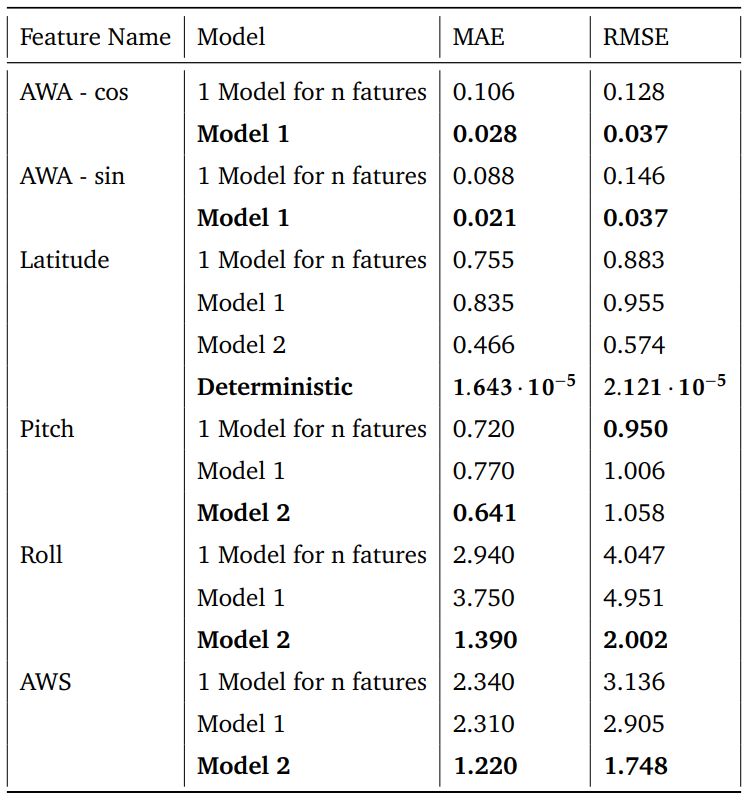
\includegraphics[width=0.7\textwidth]{figures/charles results.png}
\caption{Charles' prediction method results \cite{charles}}
\label{tbl:charles results}
\end{table}

He concluded that in general, deterministic mathematical derivations has the least error, followed by model 2, then model 1, and lastly single model for \emph{n} features. He tested model 2 in only some of the features, but it performed better in every feature tested. Error rate of different prediction methods for some of the boat features can be seen in Table \ref{tbl:charles results}. His other notable finding was that mathematical formulas do not always agree with the sensor data, which indicates that something might be wrong on the boat sensors/algorithms. Nevertheless, Charles envisions that after \emph{n} models for \emph{n} features are individually optimised, they can be integrated into a reinforcement learning framework.

\subsection{Thomas Ryder}

Following Charles' project, T-DAB employee Thomas Ryder carried on his work. Thomas' goal was to create a full pipeline which would create \emph{n} separate state estimator models, given the dataset in csv format. Charles had worked on his project using Jupyter Notebooks. Thomas converted those notebooks into concise Python scripts, plus incorporated bayesian optimization into each of the \emph{n} models like Charles suggested as a future work. Thomas' scripts now consists of the following parts, explained very briefly below:

\begin{enumerate}
  \item \textbf{Preprocessing:} Rename and select columns, convert angles to radians, scale, label tacks, split into train-validation-test segments, and downsample the data.
  \item \textbf{Optimisation:} Run Bayesian optimization for each feature within the parameters given in the config file.
  \item \textbf{Training:} Train an LSTM network with optimized hyperparameters for each feature given in the config file. Log the training history data.
  \item \textbf{Evaluation:} Make predictions using the test data, then calculate MAE and RMSE. Print information about trained models.
\end{enumerate}

According to Charles' findings of Model 2 working better on all 4 features tested, Charles decided to use Model 2 with one less final dense layer for all 18 features.

The scripts are structured better than Charles' notebooks, plus they are much easier to understand and use. However, there are some problems and tests that need to be tackled before the final models that will be used for the Reinforcement Learning Environment can be produced.


%%%%%%%%%%%%%%%%%%%%%%%%%%%%%%%%%%%%
%\chapter{Progress}
%\section{RL Framework}
After the Background Research, the planned framework to use was OpenAI's Spinning Up framework. They provide clean implementations of modern RL algorithms, and a basic interface to apply the algorithms to OpenAI Gym environments, then plot the results. However, OpenAI Spinning Up has some downsides and lack some important features that would be helpful during this project.

\subsection{RL Algorithm Implementation Differences} \label{RLF:imp-diff}
Spinning Up's main focus is education. Therefore the algorithm implementations are stripped down from the proposed versions from the original papers, so the algorithms would be easier to read and understand. Although this is good for education, the resulting algorithms do not perform up to their potential due to their simplicity. The performance of SAC which is the algorithm of choice for this project, used on different Gym environments can be seen in Figure \ref{fig:spinup-SAC}.

\begin{figure}[h]
     \centering
     \begin{subfigure}[t]{0.32\textwidth}
         \centering
         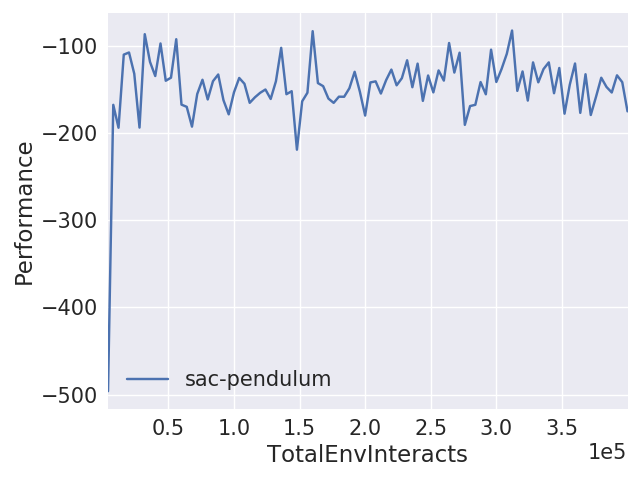
\includegraphics[width=\textwidth]{figures/rl-framework/sac-pendulum.png}
         \caption{Pendulum-v0 (Very Easy)}
     \end{subfigure}
     \hfill
     \begin{subfigure}[t]{0.32\textwidth}
         \centering
         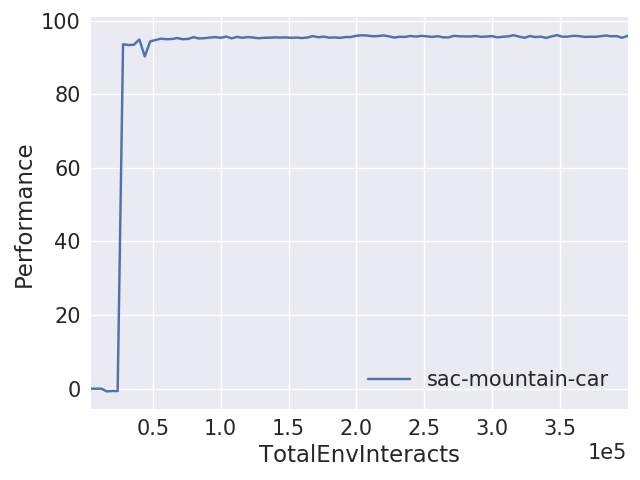
\includegraphics[width=\textwidth]{figures/rl-framework/sac-mountain-car.png}
         \caption{MountainCarContinuous-v0 (Easy)}
     \end{subfigure}
     \hfill
     \begin{subfigure}[t]{0.32\textwidth}
         \centering
         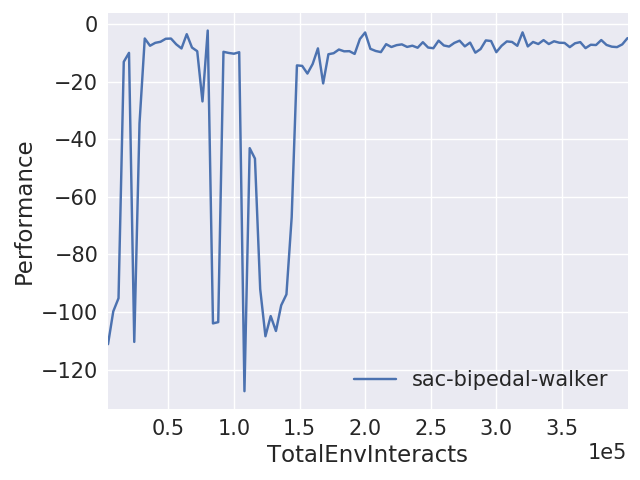
\includegraphics[width=\textwidth]{figures/rl-framework/sac-bipedal-walker.png}
         \caption{BipedalWalker-v3 (Hard)}
     \end{subfigure}
        \caption{Performance of Spinning Up implementation of SAC on different environments, using default parameters}
        \label{fig:spinup-SAC}
\end{figure}

Spinning Up implementation performs well and converges quickly on easy environments, but it provides disappointing results on the harder BipedalWalker-v3 environment. SAC is expected to have better exploration and achieve better results on BipedalWalker-v3 environment before 300.000 environment interacts \cite{gym-leaderboard}. But it never managed to escape a local minimum for a long period of training time. Considering our sailing environment will be pretty complex, Spinning Up implementation of SAC is not suitable for use on this project.

\subsection{RL Framework Features} \label{RLF:framework-features}

Spinning Up Framework lacks some important features for Reinforcement Learning. First, it does not support continuing training of a previously trained agents. This is problematic in a few ways: it costs precious time and resources to train agents from scratch every time, plus even if models are trained again from ground up, no two reinforcement learning runs will be identical because of the noise or stochasticity in the algorithms.

\begin{wrapfigure}{R}{0.5\textwidth}
\centering
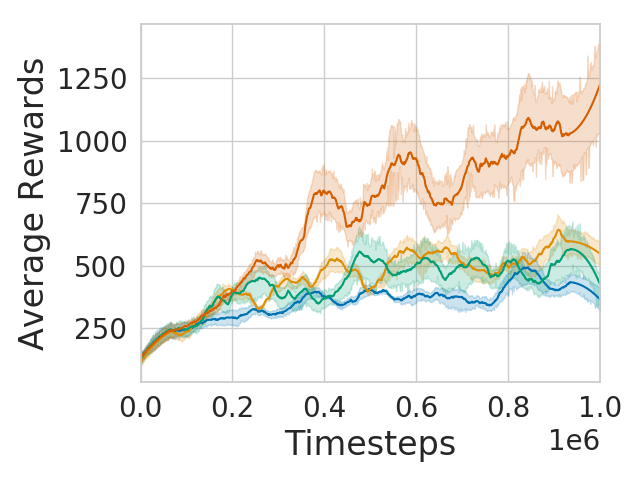
\includegraphics[width = 0.48\textwidth]{figures/rl-framework/hyperparameter-ddpg.png}
\caption{DDPG on Walker2d-v1 with random hyperparameters \cite{hyperparameter-ddpg}}
\label{fig:hyperparameter-ddpg}
\end{wrapfigure}

The second lacking feature is that there is no hyperparameter optimization support. Hyperparameters can cause huge difference in performance \cite{hyperparameter-ddpg}. A comparison of DDPG on Walker2d-v1 with random hyperparameters can be seen in Figure \ref{fig:hyperparameter-ddpg}. The best and worst performing hyperparameters have approximately 3-fold average reward difference after 1 million timesteps.

Both of these features, and probably more that will arise in the future are important for this project, so another framework with these additional features is needed.


\subsection{Stable Baselines 3}
Stable Baselines3 (SB3) is a library providing reliable implementations of state-of-the-art reinforcement learning algorithms in PyTorch, complete with a training framework 'RL Baselines3 Zoo' which contains scripts for training, evaluating agents, tuning hyperparameters, plotting results, and recording videos. \cite{stable-baselines3} 

SB3 solves both of the problems of Spinning Up Framework mentioned in sections \ref{RLF:imp-diff} and \ref{RLF:framework-features}. SB3 is focused on providing reliable implementations that can be used on Deep Reinforcement Learning Research, instead of an education focus of Spinning Up. SB3 implementations are fully functional, high quality, and they match the results of best previous implementations. A performance comparison of Soft Actor Critic implementations of Stable Baselines3 and OpenAI Spinning Up can be seen in Figure \ref{fig:spinup-vs-sb3}. We are expecting SAC to converge to 300 rewards which is the goal of this environment \cite{Bipedal-Walker-v2} in around 300.000 steps. \cite{gym-leaderboard} Stable Baselines3 implementation delivers expected results whereas the Spinning Up implementation falls short. The hyperparamaters were tuned in SB3 implementations, but weren't tuned for Spinning Up as it doesn't support hyperparameter tuning.

\begin{figure}[h]
     \centering
     \begin{subfigure}[c]{0.49\textwidth}
         \centering
         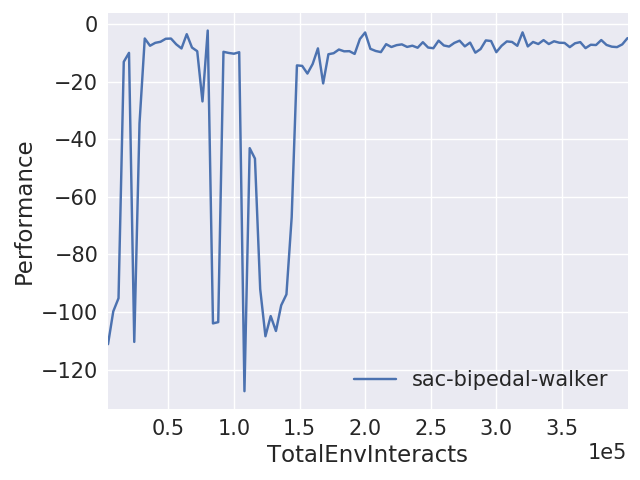
\includegraphics[width=\textwidth]{figures/rl-framework/sac-bipedal-walker.png}
         \caption{Spinning Up implementation (Default parameters) - Goal not achieved in 400.000 steps}
     \end{subfigure}
     \hfill
     \begin{subfigure}[c]{0.49\textwidth}
         \centering
         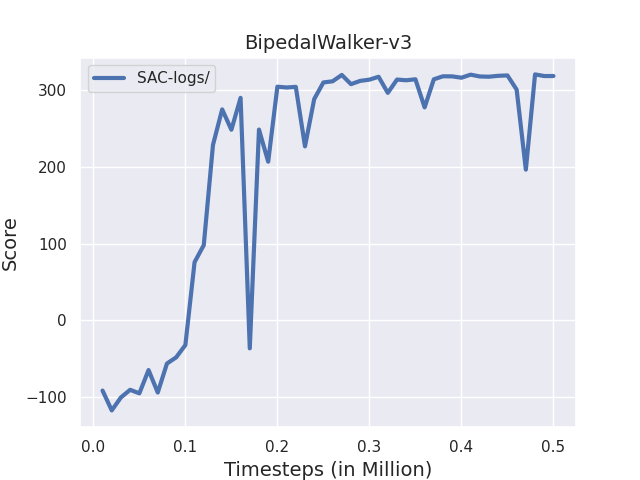
\includegraphics[width=\textwidth]{figures/rl-framework/sb3-sac-BipedalWalker-v3.png}
         \caption{Stable Baselines3 implementation (Tuned parameters) - Goal Achieved in 200.000 steps}
     \end{subfigure}
        \caption{Training Performance of Spinning Up vs Stable Baselines3 implementations of SAC. Goal Score: 300}
        \label{fig:spinup-vs-sb3}
\end{figure}

Moreover, the RL Baselines Zoo has the missing features of Spinning Up's training framework, namely hyperparameter optimization and continuing training of previously trained models. Therefore, SB3 will be the choice of RL Framework for this project from now on.

\section{State Estimator}

\section{Future Plans}

\subsection{Gym Environment}

In order to

\subsection{GoalEnv Interface}

\subsection{RL Algorithm Comparisons}

%%%%%%%%%%%%%%%%%%%%%%%%%%%%%%%%%%%%
\chapter{Data}

There are 7 datasets available for use in this project. Substantial work have been done by previous students for converting, cleaning and preprocessing the datasets. Curated information about the datasets can be found in Figures \ref{tab:datasets-practical} and \ref{tab:datasets-factual}. The information about Team Ocean dataset is recently recieved, it was referred as transat\_1 in previous student reports. 

\begin{table}[h]
\centering
\begin{tabular}{|l|l|l|l|l|c|}
\hline
\textbf{Dataset Name} & \textbf{Boat Name} & 
\textbf{\begin{tabular}[c]{@{}l@{}}Original\\Format\end{tabular}} & \textbf{\begin{tabular}[c]{@{}l@{}}Original\\Length[h]\end{tabular}} & \textbf{\begin{tabular}[c]{@{}l@{}}Cleaned\\Length[h]\end{tabular}} & \textbf{\begin{tabular}[c]{@{}l@{}}Tack\\Detection\end{tabular}} \\ \hline
RDR\_nkz    & \multirow{4}{*}{Concise 8}    & .nkz & 16    & 16    & $\ballotx$        \\ \cline{1-1} \cline{3-6}
RDR\_adrena &                               & .csv & 306   & -     & $\ballotx$        \\ \cline{1-1} \cline{3-6}
DHREAM 18   &                               & .log & 64.5  & 64.5  & $\ballotx$        \\ \cline{1-1} \cline{3-6} 
Atlantic    &                               & .nkz & 290.9 & 228.7 & $\ballotcheck$    \\ \hline
DHREAM 20   & VMB                           & .nkz & 70    & 6     & $\ballotx$        \\ \hline
Team Ocean  & Time for Oceans               & .nkz & 383.5 & 63.3  & $\ballotcheck$    \\ \hline
transat\_2  & \textit{unknown}              & .nkz & 387.5 & -     & $\ballotx$        \\ \hline
\end{tabular}
\caption{Practical information about available datasets}
\label{tab:datasets-practical}
\end{table}

\begin{table}[h]
\centering
\begin{tabular}{|l|l|l|l|l|}
\hline
\textbf{Dataset Name} & \textbf{Boat Name}         & \textbf{Boat Class}       & \textbf{Race}          & \textbf{Year} \\ \hline
RDR\_nkz              & \multirow{4}{*}{Concise 8} & \multirow{5}{*}{Class 40} & Route du Rhum          & 2018          \\ \cline{1-1} \cline{4-5} 
RDR\_adrena           &                            &                           & Route du Rhum          & 2018          \\ \cline{1-1} \cline{4-5} 
DHREAM 18             &                            &                           & DHREAM Cup             & 2018          \\ \cline{1-1} \cline{4-5} 
Atlantic              &                            &                           & \textit{boat delivery} & 2019          \\ \cline{1-2} \cline{4-5} 
DHREAM 20             & Virgin Media Business      &                           & DHREAM Cup             & 2020          \\ \hline
Team Ocean            & Time for Oceans            & \multirow{2}{*}{IMOCA 60} & Transat Jacques Vabre  & 2019          \\ \cline{1-2} \cline{4-5} 
transat\_2            & \textit{unknown}           &                           & Transat Jacques Vabre  & 2019          \\ \hline
\end{tabular}
\caption{Factual information about available datasets}
\label{tab:datasets-factual}
\end{table}

\textit{Atlantic} is the dataset with the largest available clean data, and the tack detection is already done. Therefore the \textit{Atlantic} dataset will be used in the rest of this project. You can see more information about \textit{Atlantic} in the next section. For further detail about the other datasets, see the reports of previous students \cite{roman, stan, birk, charles}. 

\section{Atlantic}
\subsection{Information and Previous Work}
The \textit{Atlantic} dataset was recorded during a boat delivery made by Jack Trigger in 2019. It was a solo delivery, therefore the autopilot was active during a large portion of the route. The data was recorded by the nke electronics system in .nkz format in 25 Hz, then converted to .csv format.

Next, the dataset was cleaned, removing unusable parts such as:
\begin{itemize}
    \item abnormal conditions such as very low wind speed
    \item corrupted parts with incomplete data
    \item sections where the boat was anchored or in harbour
\end{itemize}

The original length of the dataset was 290.9 hours, and 228.7 usuable hours have remained after cleaning done by Charles Metz \cite{charles}.

\subsection{Preprocessing Applied in State Estimator Scripts}
The datasets need to go under certain preprocessing before the state estimator models can be trained. These steps are:

\begin{itemize}
    \item \textbf{Rename and Select Columns:} Rename the columns for better clarity, and select the columns of features to be trained.
    \item \textbf{Convert Angles to sin and cos values:} When going through the end values, the angles jump between those end values such as between -180 and 180. The features that are angles are converted to sin and cos values alleviate this problem and increase model performance.
    \item \textbf{Scaling:} The values are scaled to be between -1 and 1. The data ranges and scaling applied in the scripts can be seen in Table \ref{tbl:scripts-scaling}. The ranges were thought to be physical limits by previous students, but newly available data has values above the range. See \ref{sec:future-work} - Future Work for suggestions on the issue.
    \item \textbf{Removing tacks:} The tacks in the dataset are removed.
    \item \textbf{Splitting the data:} The data is split into training, validation and testing sets. See \ref{sec:data-split-concern} for the Data Split Concerns.
    \item \textbf{Downsampling:} The data is downsampled from 25 Hz to 1 Hz to save on computing.
\end{itemize}

\begin{table}[h]
\centering
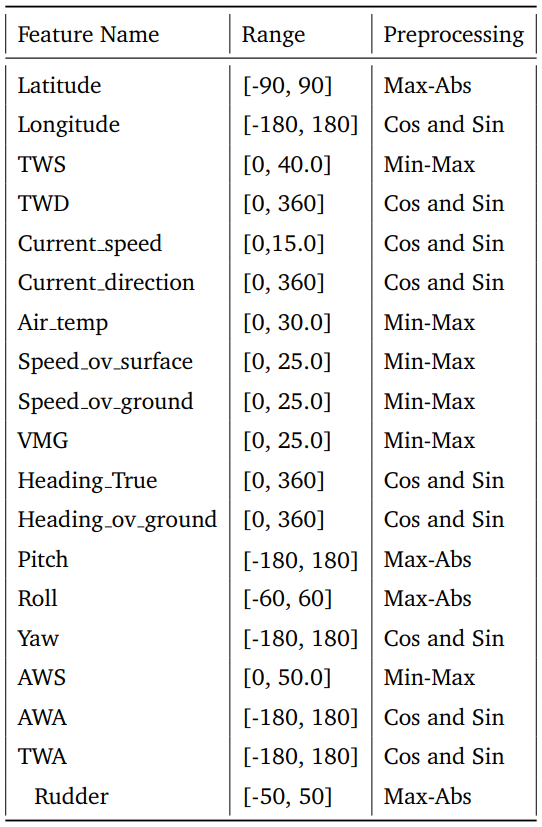
\includegraphics[width = 0.65\hsize]{figures/data scaling.png}
\caption{Updated data ranges and preprocessing applied to features}
\label{tbl:scripts-scaling}
\end{table}

\chapter{Contribution}

\section{State Estimator Scripts}
In this section contributions related to the state estimator scripts that Charles and Thomas first created will be described.

\subsection{Initial Improvements}

\subsubsection{State Estimator Bug}
When the project was handed over from Thomas, there was an error causing bug in the scripts that caused the scripts to halt without producing any results. Working together with Thomas, the problem was found to be the difference in the dataset rows that preprocessing scripts created, and the rows that optimization scripts were expecting. After fixing the bug, the scripts started working as expected in local and Azure cloud machines.

\subsubsection{Data Store}
The scripts are using local csv files as input. There was a plan to switch to using cloud databases, but the switch to databases were postponed due to the following reasons:

\begin{itemize}
  \item \textbf{Cost:} There isn't any available infrastructure in T-DAB to host the database. So, Microsoft's time-series database, InfluxDB was the choice of Database. However, keeping the database online on InfluxDB costs money.
  \item \textbf{Complexity:} The switch to cloud database adds complexity to both workflow and the code. The preprocessing code previous students have spend most of their time on work with csv files. Those csv files needs to be processed separately, uploaded to cloud database, and then the same data needs to be pulled from the database with specific querying to have the same structure with the csv files, then be fed as input to the rest of the scripts.
  \item \textbf{Time:} It will take time to implement changes required to switch to cloud databases. That time is better spend on the RL portion of the project instead.
  \item \textbf{No significant advantage:} Currently, there is no significant advantage of using stand-alone cloud database that will justify the cost, complexity, and time spent. We do not have any constant flow of data, or the need for regular analysis or reporting.
  \item \textbf{Current solution:} Currently, the race data is stored on the company SharePoint. A quick and easy way to download this data on Azure Cloud Machines was found, using a single \textit{wget} command from the terminal. This eliminates the biggest drawback of using local csv files, which is manually downloading and uploading large files. Plus it doesn't have any added cost or complexity.
\end{itemize}

A better alternative than csv files are parquet files, which are specifically designed for columnar storage format \cite{parquet}. It is more efficient than csv, and it works well with pandas used in the state estimator scripts. See \ref{sec:future-work} - Future Work.

\subsubsection{Tack Detection}
As mentioned on section \ref{sec:Stan}, when Stanislas removed the found tacks from the dataset and retrained the state estimator model, he achieved substantial improvement in the model's test results. 

To realize this improvement on our new optimized models, the scripts were modified to take the selected dataset \textit{Atlantic}'s tack bounds as input, and remove them from the train-validation-test sets. The tack bounds for Atlantic dataset were stored in a different format, which required some change in the code.

It is suggested to incorporate a tack detection system into the script pipeline. This way, the user would not have to provide the tack info for different datasets, the script will automatically find and remove them. This would also alleviate the problem of different tack bound formats. (see \ref{sec:future-work} - Future Work)

\subsection{Data Split Concern} \label{sec:data-split-concern}

There are two proposed ways of splitting the dataset into training, validation, and testing sets; named as \emph{Normal} and \emph{Segment} by Thomas. The Normal split method allocates the first 60\% of the data to training, next 20\% to validation and the last 20\% to testing. The Segment split method on the other hand, first splits the dataset into continuous segments separated by unusable areas such as tacks. Then each of those segments are individually split into train-validation-test using 60-20-20 split and then concatenated together.

\begin{figure}[h]
\centering
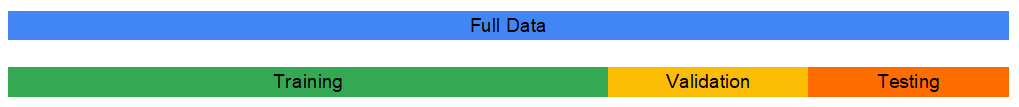
\includegraphics[width = \hsize]{figures/Contribution/Normal Split.png}
\caption{Normal Split}
\end{figure}

\begin{figure}[h]
\centering
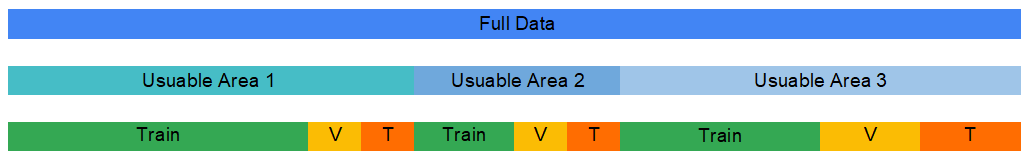
\includegraphics[width = \hsize]{figures/Contribution/Segment Split.png}
\caption{Segment Split}
\end{figure}

The data in the available datasets are logged chronologically. The nuance is that the weather and sea conditions change during the course of the races. In order to train the models on all the different sea and weather conditions, Charles has used the segment split method, as if he had used the normal split method, the models couldn't have been trained on the conditions present towards the end of the race.

Charles achieved good results using the segment split. However, one recent concern about segment split is whether it causes data leak. When using the segment split, the test data is not truly held-out. The models are trained on data that is very similar to the ones used in validation and test sets. Therefore we cannot test the performance of the models on how they would perform on truly unseen data.

The initial plan was to create two sets of models with segment and normal split methods. The resulting models would then be compared if there is a considerable difference in the error metrics. It was later learned that although undocumented in his report, Charles already compared the two split methods, and observed significantly worse results in normal split.

On a discussion with Eric Topham and Pedro Baiz, it was decided that the performance drop was due to the models not having a chance to learn about the conditions present at the end of the race. To test how the models would perform on unseen data, we will test the data trained on one race on another race. This is called the Transferability Experiment and the details can be found in section \ref{section:transferability}.

These two segment methods were the only ones that were already implemented by previous students, hence only the two were considered. There are other methods for splitting data such as forward-chaining that might achieve better results. The implementation of the segment method also have a problem. The usable areas are concatenated together, so the models are trained on data that have occasional time gaps in between. See \ref{sec:future-work} - Future Work.


\subsection{Efficiency Experiment}
At the beginning of the project, some initial tests were made to make sure the scripts were working fine on local and Azure cloud computers. It was noticed that with a small test dataset, running the scripts on CPU took shorter than running them on GPU. CTO of T-DAB, Ivan Scattergood suggested testing whether this was caused by the bigger overhead of GPU, or the scripts were straight up better optimized for CPU.

If it is just due to the multiprocessing overhead, running larger datasets on GPU should take shorter than CPU. But if it doesn't, we can conclude that the scripts are better optimized for CPU.

Therefore a series of experiments were started, trying to find the most efficient way to run the scripts; whether on single-core CPU, multi-core CPU, or GPU. Plus trying to estimate the total amount of time it would take to produce the state estimator models.

\subsubsection{Current Information}
\begin{itemize}
  \item We aim to produce 18 different state estimators. Producing each one is independent from others. They differ slightly in training time, due to the randomness of bayesian optimization and different resulting hyperparameters.
  \item With a small test dataset, using CPU takes shorter than using GPU.
\end{itemize}

\subsubsection{Hypothesis}
Running the scripts on GPU take longer with the small test dataset because of the overheads. Using bigger datasets will make GPU more efficient than CPU.

\subsubsection{Side Goal}
Predict how long the full script will take to produce all 18 models.

\subsubsection{Experimental set up and method}
\begin{enumerate}
    \item Do test runs on single threaded cpu, multi-threaded cpu, and gpu; with a small dataset and smaller optimization search space.
    \item Redo the experiments with 2x and 10x amount of data to see how it affects the runs.
    \item Lastly, test with full optimization search space with the better processing unit to estimate how long the full run will take.
\end{enumerate}

Speed\_ov\_ground was picked as the feature to train models on, as it has medium error rate in previous iterations of the models compared to the other features. It is expected to be a good example to infer how long the full run will take.

For CPU Tests, the default Azure compute instance “Standard\_DS3\_v2” with 4 cores, 14GB RAM, 28GB storage will be used. For GPU Tests, the Azure-recommended “Standard\_NC6” with 6 cores, 56GB RAM, 380GB storage will be used. The GPU is more powerful and more expensive per hour than the CPU, but it is the cheapest GPU option available on Azure.

\subsubsection{Assumptions}
\begin{itemize}
  \item Azure Mazhine Learning Computing units are consistent and does not fluctuate in performance 
  \item RAM does not have an effect on performance
\end{itemize}

\subsubsection{Results}

First of all, one should note the time needed is variable due to the randomness in Bayesian Optimization, but it should provide us with enough information for comparison.

As can be seen in Table \ref{tab:cpu-gpu} and Figure \ref{fig:cpu-gpu}, running the scripts on GPU is much faster than CPU, especially as the dataset size increases.

\begin{table}[h]
\centering
\begin{tabular}{|l|l|l|l|}
\hline
\textbf{Dataset Size} & \textbf{CPU - single threaded} & \textbf{CPU - multi threaded} & \textbf{GPU} \\ \hline
\textbf{50 MB}  & 0:01:09 & 0:01:41 & 0:01:08 \\ \hline
\textbf{100 MB} & 0:02:01 & 0:03:23 & 0:01:17 \\ \hline
\textbf{500 MB} & 0:11:24 & 0:09:12 & 0:06:08 \\ \hline
\end{tabular}
\caption{Optimization time for small search space among different processing options}
\label{tab:cpu-gpu}
\end{table}

\begin{figure}[h]
\centering
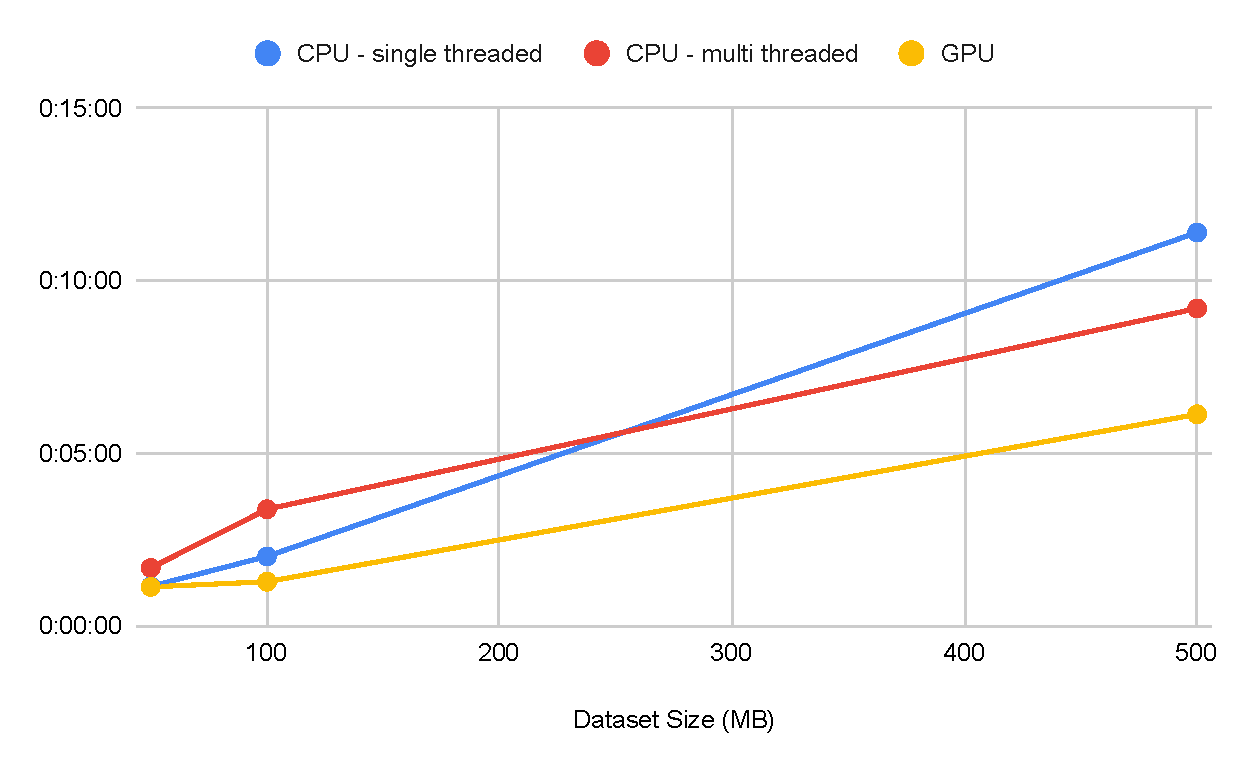
\includegraphics[width = 0.8\hsize]{figures/efficiency/cpu-gpu.pdf}
\caption{Line graph of optimization times of different processing options}
\label{fig:cpu-gpu}
\end{figure}

It is clear that hyperparameter optimization will take less time using GPU, so the further tests to estimate how long the full run will take will only be done on GPUs.

\begin{table}[h]
\centering
\begin{tabular}{|l|l|l|}
\hline
\textbf{Dataset Size} & \textbf{small search space} & \textbf{full search space} \\ \hline
\textbf{50 MB}        & 0:01:08                     & 0:12:38                    \\ \hline
\textbf{100 MB}       & 0:01:17                     & 0:16:18                    \\ \hline
\textbf{500 MB}       & 0:06:08                     & 1:18:08                    \\ \hline
\end{tabular}
\caption{Optimization times for GPU, small vs full search space}
\label{tab:gpu-search-spaces}
\end{table}

\begin{figure}[H]
\centering
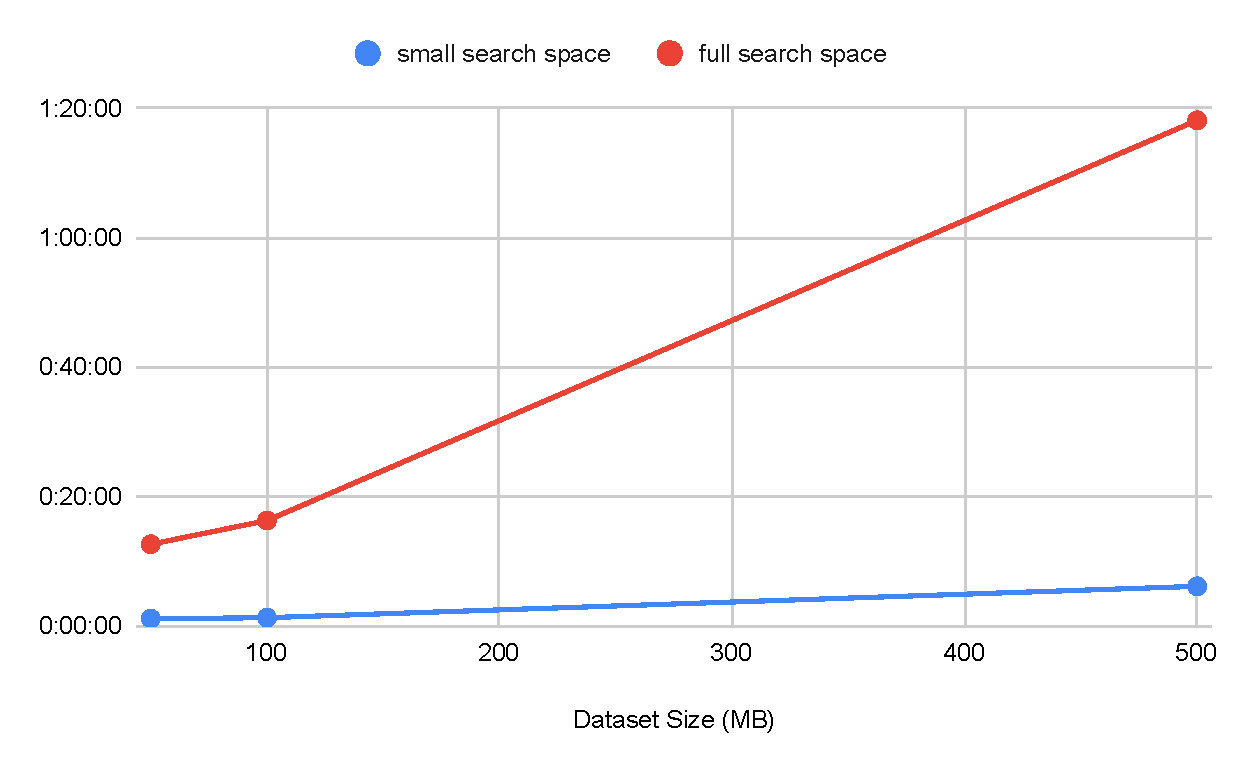
\includegraphics[width = 0.8\hsize]{figures/efficiency/gpu.pdf}
\caption{Line graph of optimization times for GPU, small vs full search space}
\label{fig:gpu}
\end{figure}

The full dataset is 12.6 GB, approximately 25 times the large dataset. The trend is pretty linear, so optimization for full dataset for 1 feature is expected to take around 32.5 hours. If all of the features take the same amount of time for optimization, all 18 features would take 585 hours, which is around 24.4 days.

Each feature is independent from each other, and running them on the same script does optimizations back to back in series. Each feature can be run on separate compute instances to save a lot of time. Assuming there is no starting fee for computing instances, and only per hour fees, this wouldn’t add much in cost either.

\subsubsection{Conclusion}
The hypothesis was true, GPU takes shorter in bigger datasets, and the gap is expected to grow in even bigger datasets.

From the results of this experiment, running the full dataset for all features is expected to take around 24.4 days on a single compute, but they can also be run on separate compute instances to save time with no considerable drawback.

\subsubsection{Next Step}
The full optimization and training runs for all 18 features will be run on multiple Azure Cloud GPUs in parallel.

\section{Optimized Models}

After the efficiency tests were completed and GPU was chosen as the choice of processing unit, the full optimization and training run was started. T-DAB has received credits from Microsoft that can be spent on Azure ML platform for Innovation use. Therefore, the default NVIDIA Tesla K80 GPUs available on Azure ML platform were used to optimize and train the models. The result of the efficiency test points that multiple GPUs can be used in parallel. The maximum number of GPUs in the innovation account quota was used and the models were trained on 3 seperate NVIDIA Tesla K80 GPUs.

\begin{table}[htbp]
\centering
\begin{tabular}{|l|l|l|l|}
\hline
\textbf{Feature} &
  \textbf{Model} &
  \textbf{MAE} &
  \textbf{RMSE} \\ \hline
AWS &
  \begin{tabular}[c]{@{}l@{}}Model 2\\ \textbf{optimized}\end{tabular} &
  \begin{tabular}[c]{@{}l@{}}1.220\\ 0.614\end{tabular} &
  \begin{tabular}[c]{@{}l@{}}1.748\\ 0.785\end{tabular} \\ \hline
Yaw\_cos &
  \begin{tabular}[c]{@{}l@{}}Model 1\\ \textbf{optimized}\end{tabular} &
  \begin{tabular}[c]{@{}l@{}}0.007\\ 0.007\end{tabular} &
  \begin{tabular}[c]{@{}l@{}}0.051\\ 0.023\end{tabular} \\ \hline
Yaw\_sin &
  \begin{tabular}[c]{@{}l@{}}Model 1\\ \textbf{optimized}\end{tabular} &
  \begin{tabular}[c]{@{}l@{}}0.040\\ 0.021\end{tabular} &
  \begin{tabular}[c]{@{}l@{}}0.053\\ 0.034\end{tabular} \\ \hline
Pitch &
  \begin{tabular}[c]{@{}l@{}}\textbf{Model 2}\\ optimized\end{tabular} &
  \begin{tabular}[c]{@{}l@{}}0.641\\ 1.367\end{tabular} &
  \begin{tabular}[c]{@{}l@{}}1.058\\ 1.822\end{tabular} \\ \hline
AWA\_cos &
  \begin{tabular}[c]{@{}l@{}}\textbf{Model 1}\\ optimized\end{tabular} &
  \begin{tabular}[c]{@{}l@{}}0.028\\ 0.040\end{tabular} &
  \begin{tabular}[c]{@{}l@{}}0.037\\ 0.056\end{tabular} \\ \hline
AWA\_sin &
  \begin{tabular}[c]{@{}l@{}}\textbf{Model 1}\\ optimized\end{tabular} &
  \begin{tabular}[c]{@{}l@{}}0.021\\ 0.031\end{tabular} &
  \begin{tabular}[c]{@{}l@{}}0.037\\ 0.045\end{tabular} \\ \hline
Roll &
  \begin{tabular}[c]{@{}l@{}}Model 2\\ \textbf{optimized}\end{tabular} &
  \begin{tabular}[c]{@{}l@{}}1.390\\ 1.470\end{tabular} &
  \begin{tabular}[c]{@{}l@{}}2.002\\ 1.910\end{tabular} \\ \hline
Heading\_ov\_ground\_cos &
  \begin{tabular}[c]{@{}l@{}}Model 1\\ \textbf{optimized}\end{tabular} &
  \begin{tabular}[c]{@{}l@{}}0.037\\ 0.011\end{tabular} &
  \begin{tabular}[c]{@{}l@{}}0.076\\ 0.025\end{tabular} \\ \hline
Heading\_ov\_ground\_sin &
  \begin{tabular}[c]{@{}l@{}}Model 1\\ \textbf{optimized}\end{tabular} &
  \begin{tabular}[c]{@{}l@{}}0.020\\ 0.013\end{tabular} &
  \begin{tabular}[c]{@{}l@{}}0.044\\ 0.048\end{tabular} \\ \hline
Speed\_ov\_ground &
  \begin{tabular}[c]{@{}l@{}}Model 1\\ \textbf{optimized}\end{tabular} &
  \begin{tabular}[c]{@{}l@{}}0.820\\ 0.132\end{tabular} &
  \begin{tabular}[c]{@{}l@{}}1.154\\ 0.205\end{tabular} \\ \hline
Heading\_Mag\_cos &
  \begin{tabular}[c]{@{}l@{}}-\\ optimized\end{tabular} &
  \begin{tabular}[c]{@{}l@{}}-\\ 0.016\end{tabular} &
  \begin{tabular}[c]{@{}l@{}}-\\ 0.024\end{tabular} \\ \hline
Heading\_Mag\_sin &
  \begin{tabular}[c]{@{}l@{}}-\\ optimized\end{tabular} &
  \begin{tabular}[c]{@{}l@{}}-\\ 0.014\end{tabular} &
  \begin{tabular}[c]{@{}l@{}}-\\ 0.023\end{tabular} \\ \hline
VMG &
  \begin{tabular}[c]{@{}l@{}}\textbf{Model 1}\\ optimized\end{tabular} &
  \begin{tabular}[c]{@{}l@{}}0.520\\ 0.767\end{tabular} &
  \begin{tabular}[c]{@{}l@{}}0.866\\ 1.100\end{tabular} \\ \hline
TWA\_cos &
  \begin{tabular}[c]{@{}l@{}}Model 1\\ \textbf{optimized}\end{tabular} &
  \begin{tabular}[c]{@{}l@{}}0.026\\ 0.022\end{tabular} &
  \begin{tabular}[c]{@{}l@{}}0.036\\ 0.030\end{tabular} \\ \hline
TWA\_sin &
  \begin{tabular}[c]{@{}l@{}}Model 1\\ \textbf{optimized}\end{tabular} &
  \begin{tabular}[c]{@{}l@{}}0.021\\ 0.016\end{tabular} &
  \begin{tabular}[c]{@{}l@{}}0.034\\ 0.024\end{tabular} \\ \hline
Speed\_ov\_surface &
  \begin{tabular}[c]{@{}l@{}}Model 1\\ \textbf{optimized}\end{tabular} &
  \begin{tabular}[c]{@{}l@{}}1.200\\ 0.231\end{tabular} &
  \begin{tabular}[c]{@{}l@{}}1.846\\ 0.347\end{tabular} \\ \hline
Heading\_True\_cos &
  \begin{tabular}[c]{@{}l@{}}Model 1\\ \textbf{optimized}\end{tabular} &
  \begin{tabular}[c]{@{}l@{}}0.017\\ 0.010\end{tabular} &
  \begin{tabular}[c]{@{}l@{}}0.045\\ 0.018\end{tabular} \\ \hline
Heading\_True\_sin &
  \begin{tabular}[c]{@{}l@{}}Model 1\\ \textbf{optimized}\end{tabular} &
  \begin{tabular}[c]{@{}l@{}}0.017\\ 0.012\end{tabular} &
  \begin{tabular}[c]{@{}l@{}}0.038\\ 0.020\end{tabular} \\ \hline
\end{tabular}
\caption{Charles' best performing models on smaller DHREAM18 dataset vs new optimized models trained and tested on larger Atlantic dataset}
\label{tab:opt-model}
\end{table}

18 models were trained for 18 features. The error rates of the optimized models can be seen in Table \ref{tab:opt-model}, compared to the error rates of Charles' best performing models. The new models were trained and tested on the larger \textit{Atlantic} dataset, whereas Charles' models were trained and tested on the smaller \textit{DHREAM 18} dataset. Thus it is not a one to one comparison, and because the optimized models were trained and tested on a larger dataset with a more variaty of conditions, we might even expect larger error rates. Nevertheless many of the features have same or lower error rates, which is a great success, except from Pitch, AWA\_cos, AWA\_sin, and VMG models that have higher error rates.

The efficiency test results suggested that the optimization would take around 34.5 hours for every feature. In the original scripts and during the efficiency tests, there were logging messages about GPU jobs, printing hundreds of times each second to console. Printing has a surprising effect on time taken by a program, more than a novice engineer might expect. Before starting the runs on Azure cloud GPUs, these logging prints were removed. 

\begin{figure}[h]
\centering
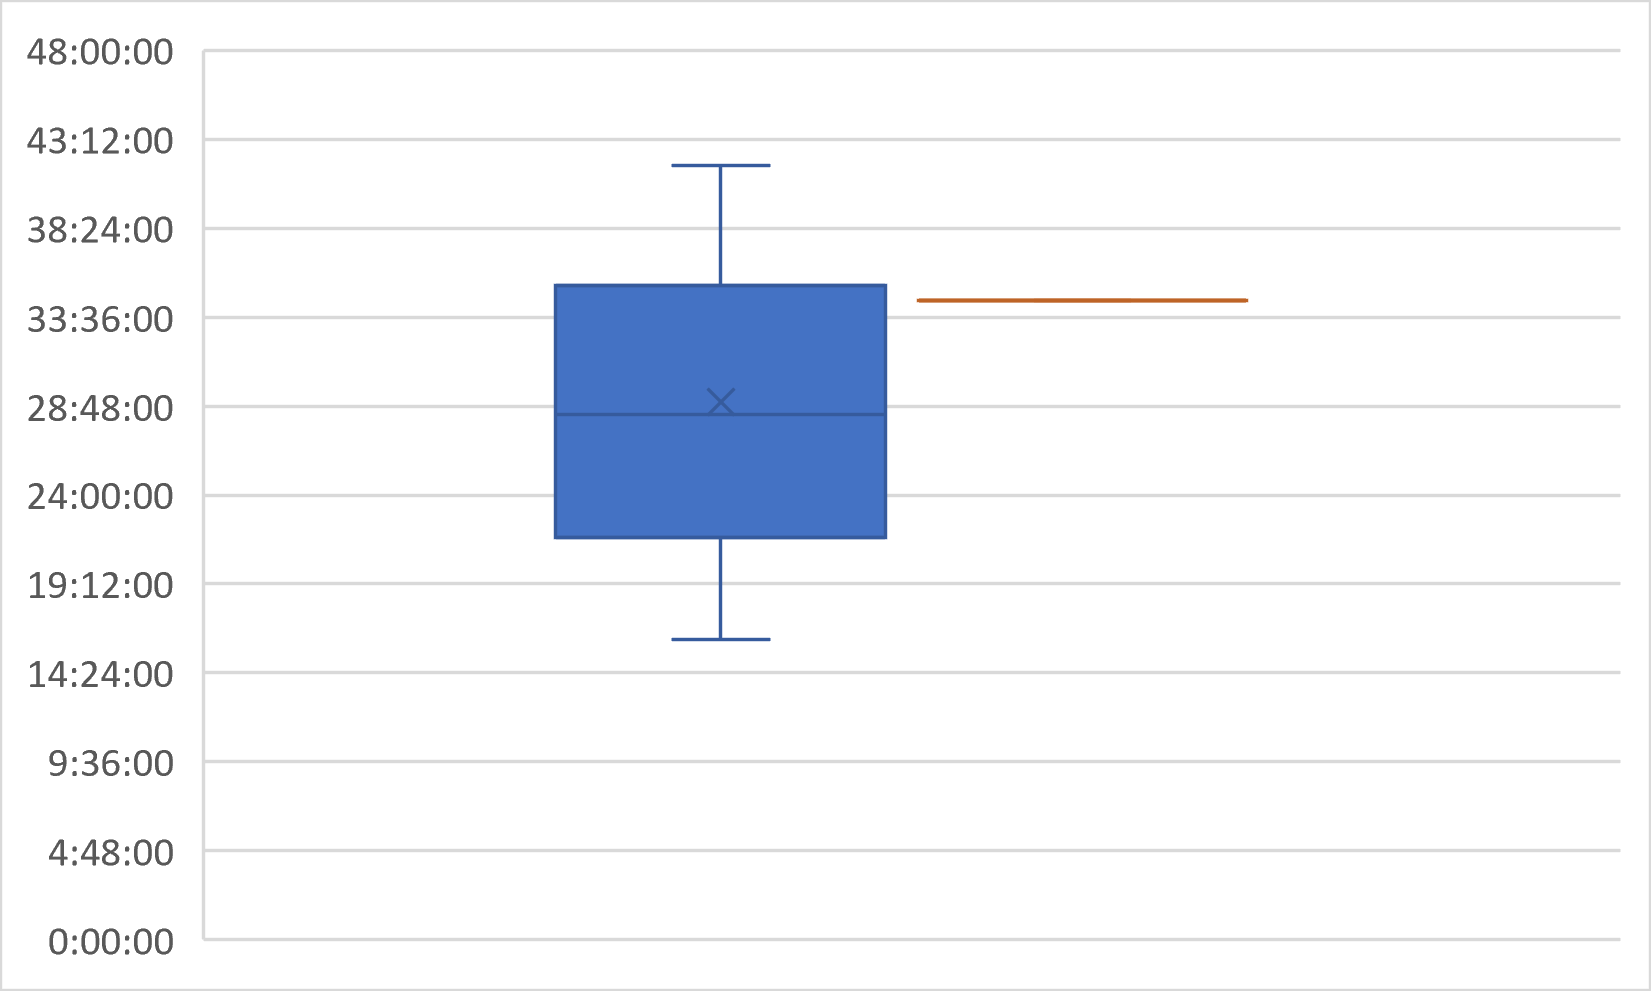
\includegraphics[width = 0.8\hsize]{figures/Contribution/Opt-time-box-whisker.png}
\caption{Optimization time box-whisker plot compared to estimated time(orange)}
\label{fig:opt-time}
\end{figure}

In the resulting models, the average optimization duration was 29:01:16, minimum was 16:11:35, and maximum was 41:46:53. A box whisker plot of the optimization times, compared to the estimated time from the efficiency tests can be seen in Figure \ref{fig:opt-time}. As expected, the range is pretty high due to randomness in Bayesian randomness. However, judging from the plot, the estimated time was accurate and removing the excessive log prints were effective.

The full details of the runs, including optimization times, training times, error metrics, and the resulting hyperparameters for all features can be found in Appendix \ref{app:azure-runs}.

\subsection{Performance Comparison}

To be able to judge the effect of hyperparameter optimization, some features were selected and trained on the same \textit{Atlantic} dataset with the same model architecture, but with the hyperparameters Charles have used. Only 6 features were trained, as training costs resources and money, plus 6 features should be enough to provide us with a good performance comparison. The performance comparison of the 6 features can be seen in Table \ref{tab:hyperparam-comparison}.

\begin{table}[h]
\centering
\begin{tabular}{|l|l|l|l|}
\hline
\textbf{Feature} &
  \textbf{Hyperparameters} &
  \textbf{MAE} &
  \textbf{RMSE} \\ \hline
AWS &
  \begin{tabular}[c]{@{}l@{}}charles\\ optimized\end{tabular} &
  \begin{tabular}[c]{@{}l@{}}1.000\\ 0.614\end{tabular} &
  \begin{tabular}[c]{@{}l@{}}1.234\\ 0.785\end{tabular} \\ \hline
Yaw\_cos &
  \begin{tabular}[c]{@{}l@{}}charles\\ optimized\end{tabular} &
  \begin{tabular}[c]{@{}l@{}}0.006\\ 0.007\end{tabular} &
  \begin{tabular}[c]{@{}l@{}}0.028\\ 0.023\end{tabular} \\ \hline
Yaw\_sin &
  \begin{tabular}[c]{@{}l@{}}charles\\ optimized\end{tabular} &
  \begin{tabular}[c]{@{}l@{}}0.027\\ 0.021\end{tabular} &
  \begin{tabular}[c]{@{}l@{}}0.038\\ 0.034\end{tabular} \\ \hline
Roll &
  \begin{tabular}[c]{@{}l@{}}charles\\ optimized\end{tabular} &
  \begin{tabular}[c]{@{}l@{}}4.429\\ 1.470\end{tabular} &
  \begin{tabular}[c]{@{}l@{}}5.218\\ 1.910\end{tabular} \\ \hline
Heading\_ov\_ground\_cos &
  \begin{tabular}[c]{@{}l@{}}charles\\ optimized\end{tabular} &
  \begin{tabular}[c]{@{}l@{}}0.024\\ 0.011\end{tabular} &
  \begin{tabular}[c]{@{}l@{}}0.038\\ 0.025\end{tabular} \\ \hline
Heading\_ov\_ground\_sin &
  \begin{tabular}[c]{@{}l@{}}charles\\ optimized\end{tabular} &
  \begin{tabular}[c]{@{}l@{}}0.031\\ 0.013\end{tabular} &
  \begin{tabular}[c]{@{}l@{}}0.052\\ 0.048\end{tabular} \\ \hline
\end{tabular}
\caption{Performance of the models, charles' vs optimized hyperparameters}
\label{tab:hyperparam-comparison}
\end{table}

\begin{figure}[h]
\centering
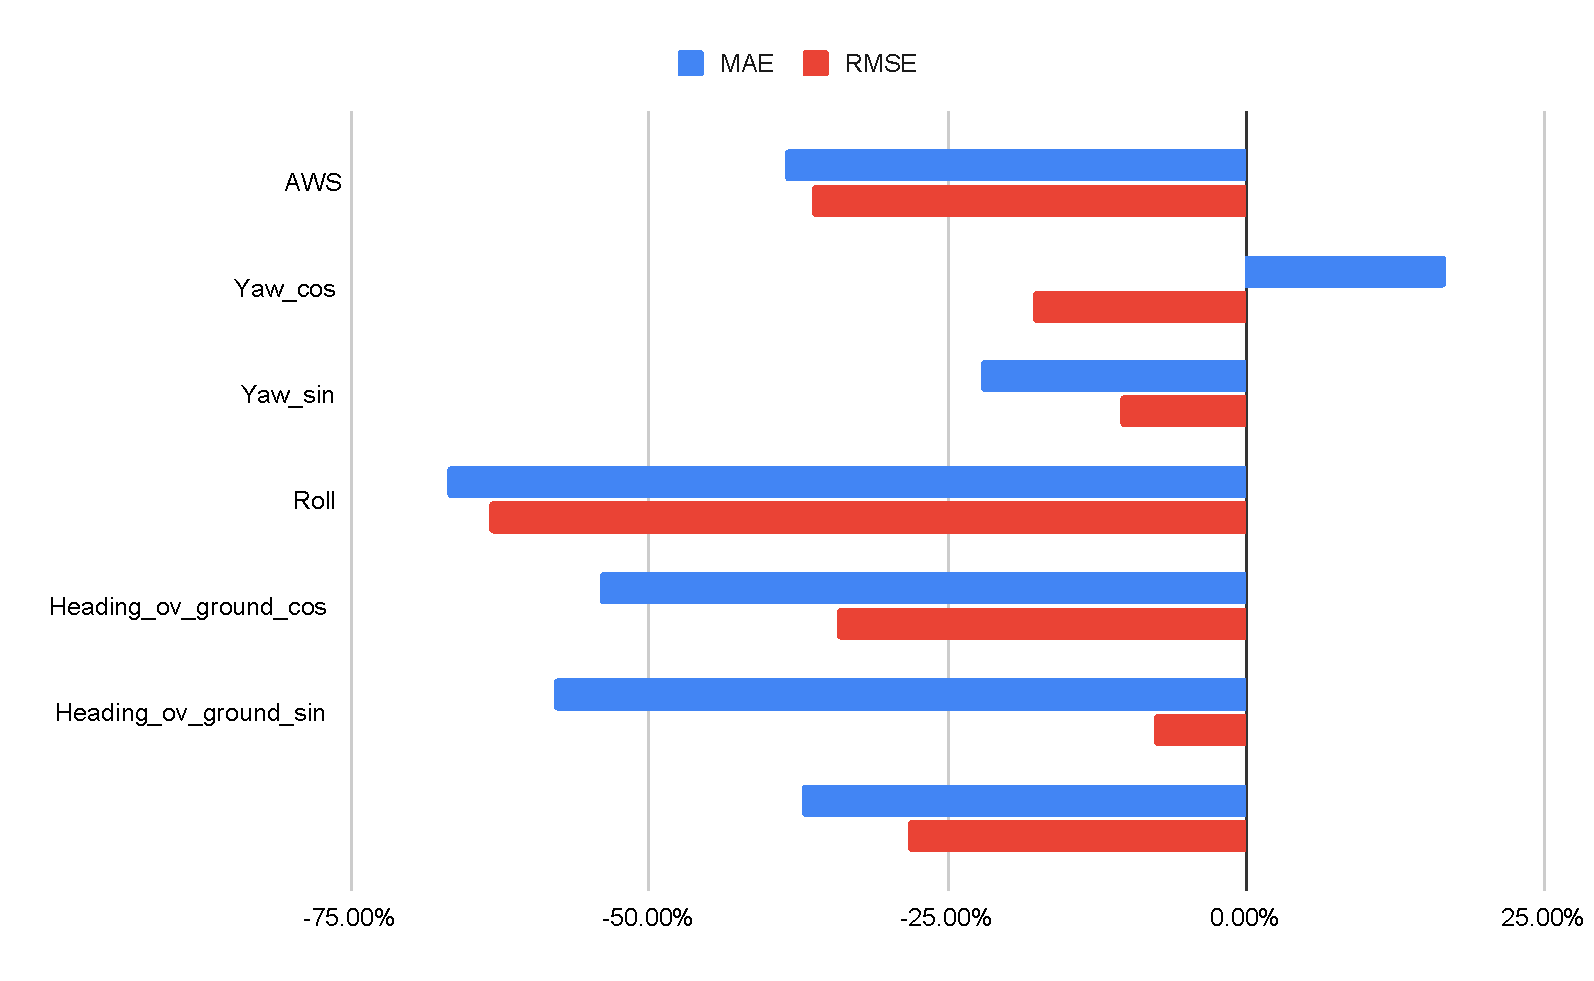
\includegraphics[width = 0.9\hsize]{figures/Contribution/opt-perf.pdf}
\caption{Percentage change in error metrics for each feature tested}
\label{fig:opt-perf}
\end{figure}

The average MAE decreased by 37.3\%, whereas the average RMSE decreased by 28.34\% among the features tested. It is clear that the optimization had a significant effect on the performance. The percentage changes in test metrics for each feature can be seen in Figure \ref{fig:opt-perf}. A negative change means that optimized models have less error rates.

Among the 6 features tested, only Yaw\_cos MAE performs worse with the optimized parameters. There might be similar instances in the features that were not tested. This might be due to the optimization setup. The optimization covers a wide search space suggested by Charles, and consists of 10 exploration, 10 exploitation steps as suggested by Thomas. These steps might not be enough to find the best possible set of hyperparameters given the size of the search space. Further optimizations can be made by tuning the search space and number of optimization steps according to the resulting hyperparameters. See \ref{sec:future-work} - Future Work.


\section{Transferability Experiment} \label{section:transferability}

This section is about the Transferability Experiment conducted to see how well the models trained on one dataset can predict the boat features using data from another dataset.

\subsubsection{Current Information}
\begin{itemize}
  \item Each dataset belongs to another race/boat transfer, so the sea, wind and the boat trim conditions are different.
  \item The new, optimized models were trained on the \textit{Atlantic} dataset, which were recorded by nke instruments and software. \textit{Atlantic} is the largest clean dataset currently available.
  \item Charles have previously tested and found that the models trained on one dataset are not transferable to another dataset recorded on the same boat with a different electronics system.
\end{itemize}

\subsubsection{Hypothesis}
The new models have optimized hyperparameters and were trained on a larger dataset.
\begin{itemize}
  \item \textbf{Hypothesis 1:} The new models will be able to predict the boat states of another dataset that were recorded on the same boat with the same electronics system, with a similar error rate.
  \item \textbf{Hypothesis 2:} The new models will be able to predict the boat states of another dataset that were recorded on the same boat with the same electronics system, with a similar error rate, on the sections that have similar environmental conditions.
\end{itemize}

\subsubsection{Assumptions}
Charles' suggested essential features describing the physical environment, which are: True Wind Speed, True Wind Angle, Apparent Wind Angle, and Pitch, provide an accurate and sufficient description of the environment. More information about these essential features can be found in Appendix \ref{app:essential-features}.

\subsubsection{Experimental set up and methods}
To test this hypothesis, we need a dataset which was recorded on the same boat with the same electronics system and format as the \textit{Atlantic} dataset the models were trained on. Looking at Figure \ref{tab:datasets-practical} in the Available Datasets Section, we can see that the \textit{RDR\_nkz} dataset, suits these requirements. Thus it was chosen as the dataset to make the experiments.

To test both of the hypotheses, A new dataset was created, named \textit{RDR\_nkz (Atlantic conditions)}, by selecting parts from the RDR\_nkz dataset, which have the mentioned four essential features in the range of what is present in the \textit{Atlantic} dataset. For a detailed explanation of how \textit{RDR\_nkz (Atlantic conditions)} was created, see Appendix.


\subsubsection{Results}

The error rates for each feature can be seen in Table \ref{tab:transferability} and the average error rates for different testing datasets is available in Figure \ref{fig:transferability-avg-chart}.

The error rates on \textit{RDR\_nkz} dataset are over four times the rates on the \textit{Atlantic} dataset. Moreover, the error rates of \textit{RDR\_nkz (Atlantic conditions)}, which was created to have similar conditions to the \textit{Atlantic} dataset, are even higher than the full \textit{RDR\_nkz} dataset.

\begin{table}[htbp]
\centering
\rowcolors{2}{gray!20}{white}
\begin{tabular}{|l|l|l|l|l|l|l|}
\hline
\multicolumn{1}{|r|}{\textbf{Test Set:}} &
  \multicolumn{2}{c|}{\textbf{Atlantic}} &
  \multicolumn{2}{c|}{\textbf{RDR\_nkz}} &
  \multicolumn{2}{c|}{\textbf{\begin{tabular}[c]{@{}c@{}}RDR\_nkz\\ (Atlantic \\ conditions)\end{tabular}}} \\ \hline
                         & MAE   & RMSE  & MAE   & RMSE  & MAE   & RMSE  \\ \hline
AWS                      & 0.614 & 0.785 & 10.44 & 11.48 & 13.11 & 13.83 \\ \hline
Yaw\_cos                 & 0.007 & 0.023 & 0.025 & 0.029 & 0.025 & 0.030 \\ \hline
Yaw\_sin                 & 0.021 & 0.034 & 0.165 & 0.182 & 0.221 & 0.231 \\ \hline
Pitch                    & 1.367 & 1.822 & 6.697 & 7.643 & 9.904 & 10.39 \\ \hline
AWA\_cos                 & 0.040 & 0.056 & 0.175 & 0.242 & 0.073 & 0.095 \\ \hline
AWA\_sin                 & 0.031 & 0.045 & 0.134 & 0.170 & 0.085 & 0.111 \\ \hline
Roll                     & 1.470 & 1.910 & 7.589 & 8.998 & 11.76 & 12.40 \\ \hline
Heading\_ov\_ground\_cos & 0.011 & 0.025 & 0.193 & 0.251 & 0.099 & 0.113 \\ \hline
Heading\_ov\_ground\_sin & 0.013 & 0.048 & 0.538 & 0.699 & 0.518 & 0.707 \\ \hline
Speed\_ov\_ground  & 0.132 & 0.205 & 2.094 & 2.367 & 2.580 & 2.742 \\ \hline
Heading\_Mag\_cos  & 0.016 & 0.024 & 0.289 & 0.407 & 0.167 & 0.216 \\ \hline
Heading\_Mag\_sin  & 0.014 & 0.023 & 0.357 & 0.391 & 0.357 & 0.407 \\ \hline
VMG                & 0.767 & 1.100 & 3.917 & 4.379 & 2.276 & 2.698 \\ \hline
TWA\_cos           & 0.022 & 0.030 & 0.118 & 0.140 & 0.111 & 0.125 \\ \hline
TWA\_sin           & 0.016 & 0.024 & 0.137 & 0.159 & 0.213 & 0.226 \\ \hline
Speed\_ov\_surface & 0.231 & 0.347 & 2.433 & 2.746 & 3.644 & 3.820 \\ \hline
Heading\_True\_cos & 0.010 & 0.018 & 0.153 & 0.225 & 0.080 & 0.103 \\ \hline
Heading\_True\_sin & 0.012 & 0.020 & 0.320 & 0.412 & 0.357 & 0.458 \\ \hline
\end{tabular}
\caption{Full error rate data of the transferability experiment for all features}
\label{tab:transferability}
\end{table}


\begin{figure}[htbp]
\centering
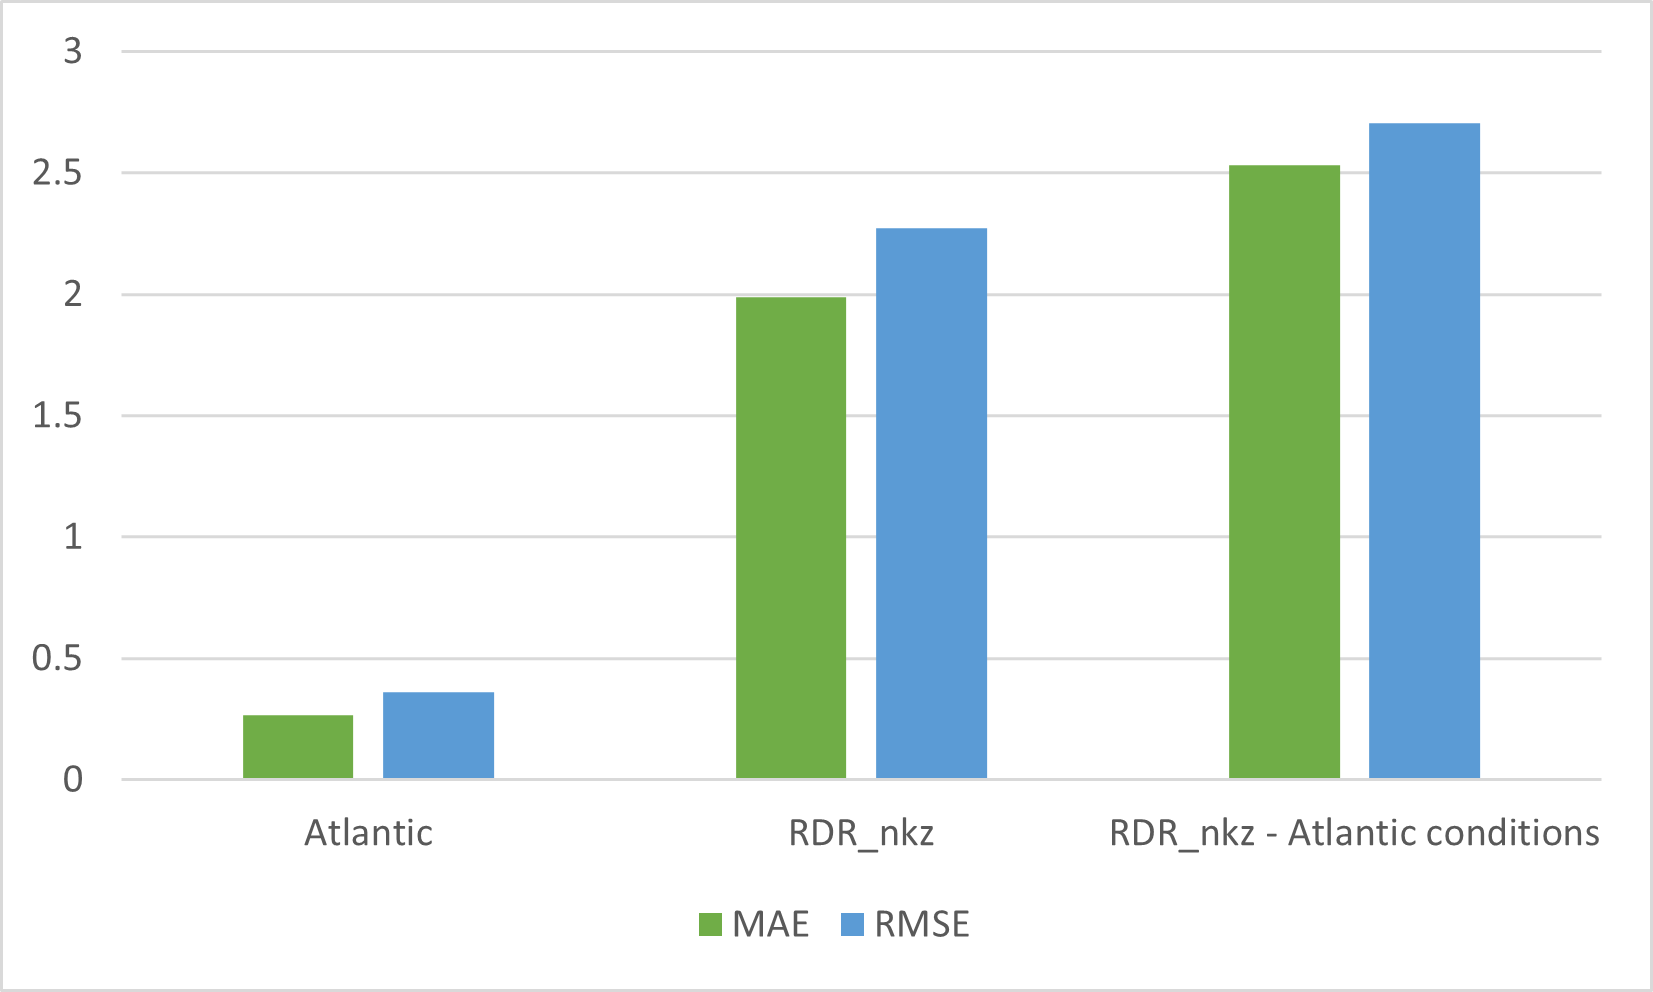
\includegraphics[width = \hsize]{figures/transferability/transferability chart.png}
\caption{Average error rates on different testsets}
\label{fig:transferability-avg-chart}
\end{figure}

\subsubsection{Conclusion}
Both of the hypotheses were wrong, as the models trained on the \textit{Atlantic} dataset have drastically higher error rates on both the \textit{RDR\_nkz} dataset, which was recorded on the same boat and same electronics system; and on the \textit{RDR\_nkz (Atlantic conditions)} dataset, which also have similar environmental conditions.

A further takeaway is that Charles' suggested essential features describing the physical environment are not sufficient for transferability among datasets, as the error rates of \textit{RDR\_nkz (Atlantic conditions)} are higher than \textit{RDR\_nkz} error rates.

\subsubsection{Next Steps}
The state estimator models we have can only predict succesfully on \textit{Atlantic} data. Therefore in the RL environment that will be created, the data from \textit{Atlantic} dataset will be used.

Suggestions on how to improve the state estimators so it can perform better can be found in \ref{sec:future-work} - Future Work.

\section{RL Framework}
After the Background Research, the planned Reinforcement Learning framework to use was OpenAI's Spinning Up framework \cite{SpinningUp2018}. They provide clean implementations of modern RL algorithms, and a basic interface to apply the algorithms to OpenAI Gym environments, then plot the results. However, OpenAI Spinning Up has some downsides and lack some important features that would be helpful during this project.

\subsection{RL Algorithm Implementation Differences} \label{RLF:imp-diff}
Spinning Up's main focus is education. Therefore the algorithm implementations are stripped down from the proposed versions from the original papers, so the algorithms would be easier to read and understand. Although this is good for education, the resulting algorithms do not perform up to their potential due to their simplicity. The performance of SAC which is the algorithm of choice for this project, used on different Gym environments can be seen in Figure \ref{fig:spinup-SAC}.

\begin{figure}[h]
     \centering
     \begin{subfigure}[t]{0.32\textwidth}
         \centering
         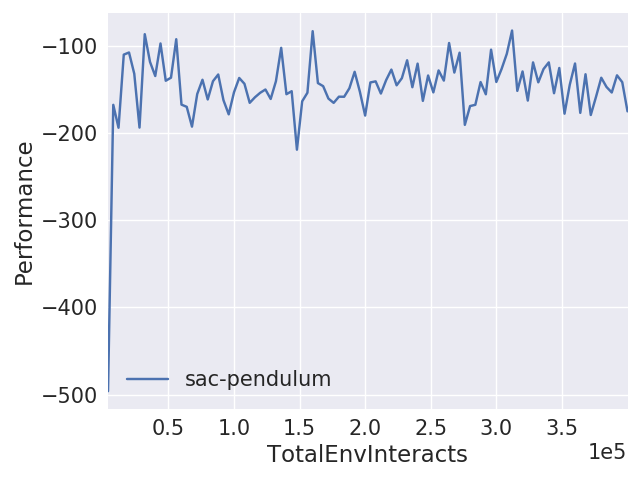
\includegraphics[width=\textwidth]{figures/rl-framework/sac-pendulum.png}
         \caption{Pendulum-v0 (Very Easy)}
     \end{subfigure}
     \hfill
     \begin{subfigure}[t]{0.32\textwidth}
         \centering
         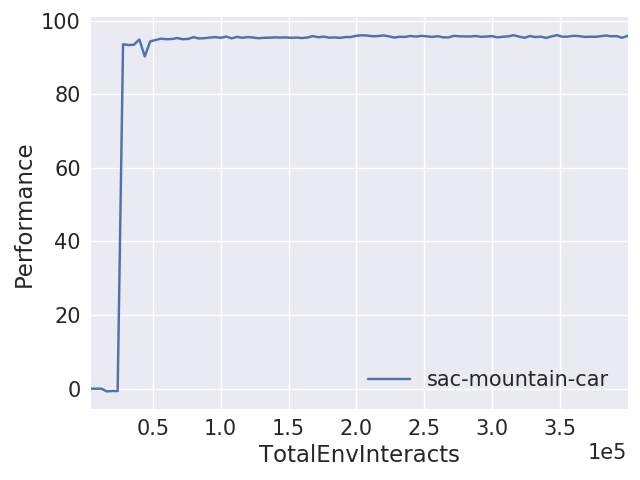
\includegraphics[width=\textwidth]{figures/rl-framework/sac-mountain-car.png}
         \caption{MountainCarContinuous-v0 (Easy)}
     \end{subfigure}
     \hfill
     \begin{subfigure}[t]{0.32\textwidth}
         \centering
         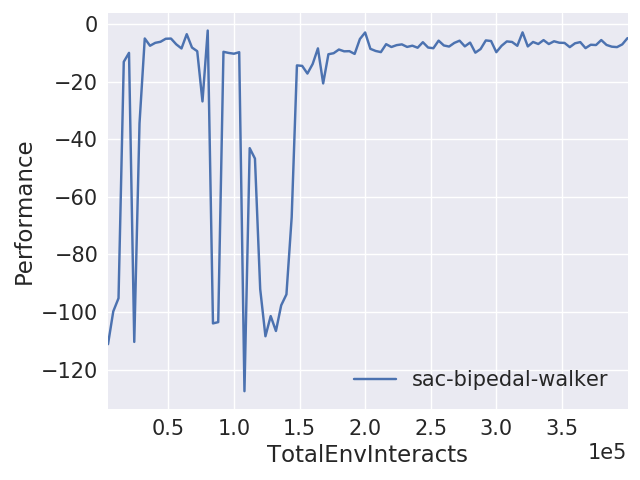
\includegraphics[width=\textwidth]{figures/rl-framework/sac-bipedal-walker.png}
         \caption{BipedalWalker-v3 (Hard)}
     \end{subfigure}
        \caption{Performance of Spinning Up implementation of SAC on different environments, using default parameters}
        \label{fig:spinup-SAC}
\end{figure}

Spinning Up implementation performs well and converges quickly on easy environments, but it provides disappointing results on the harder BipedalWalker-v3 environment. SAC is expected to have better exploration and achieve better results on BipedalWalker-v3 environment before 300.000 environment interacts \cite{gym-leaderboard}. But it never managed to escape a local minimum for a long period of training time. Considering our sailing environment will be pretty complex, Spinning Up implementation of SAC is not suitable for use on this project.


\subsection{RL Framework Features} \label{RLF:framework-features}

Spinning Up Framework lacks some important features for Reinforcement Learning. First, it does not support continuing training of a previously trained agents. This is problematic in a few ways: it costs precious time and resources to train agents from scratch every time, plus even if models are trained again from ground up, no two reinforcement learning runs will be identical because of the noise or stochasticity in the algorithms.

The second lacking feature is that there is no hyperparameter optimization support. Hyperparameters can cause huge difference in performance \cite{hyperparameter-ddpg}. A comparison of DDPG on Walker2d-v1 with random hyperparameters can be seen in Figure \ref{fig:hyperparameter-ddpg}. The best and worst performing hyperparameters have approximately 3-fold average reward difference after 1 million timesteps.

\begin{figure}[h]
\centering
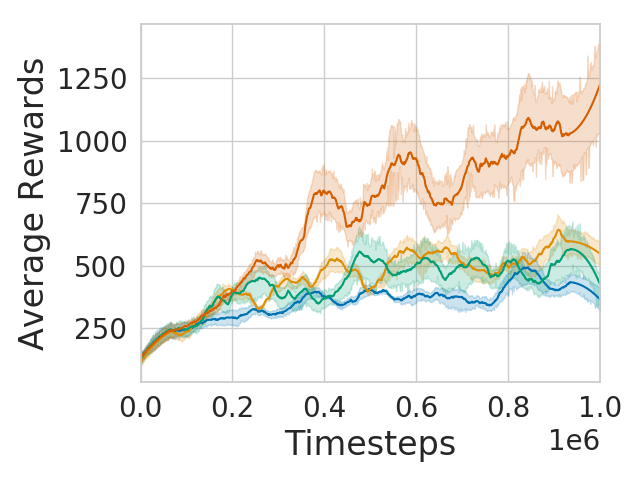
\includegraphics[width = 0.55\textwidth]{figures/rl-framework/hyperparameter-ddpg.png}
\caption{DDPG on Walker2d-v1, each color uses a different set of randomized hyperparameters \cite{hyperparameter-ddpg}}
\label{fig:hyperparameter-ddpg}
\end{figure}

Both of these features, and probably more that will arise in the future are important for this project, so another framework with these additional features is needed.


\subsection{Stable Baselines 3}
Stable Baselines3 (SB3) is a library providing reliable implementations of state-of-the-art reinforcement learning algorithms in PyTorch, complete with a training framework 'RL Baselines3 Zoo' which contains scripts for training, evaluating agents, tuning hyperparameters, plotting results, and recording videos \cite{stable-baselines3}.

SB3 solves both of the problems of Spinning Up Framework mentioned in sections \ref{RLF:imp-diff} and \ref{RLF:framework-features}. SB3 is focused on providing reliable implementations that can be used on Deep Reinforcement Learning Research, instead of an education focus of Spinning Up. SB3 implementations are fully functional, high quality, and they match the results of best previous implementations. A performance comparison of Soft Actor Critic implementations of Stable Baselines3 and OpenAI Spinning Up can be seen in Figure \ref{fig:spinup-vs-sb3}. We are expecting SAC to converge to 300 score which is the goal of this environment \cite{Bipedal-Walker-v2} in around 300.000 steps \cite{gym-leaderboard}. Stable Baselines3 implementation delivers expected results whereas the Spinning Up implementation falls short. The hyperparamaters were tuned in SB3 implementations, but weren't tuned for Spinning Up as it doesn't support hyperparameter tuning.

\begin{figure}[h]
     \centering
     \begin{subfigure}[t]{0.49\textwidth}
         \centering
         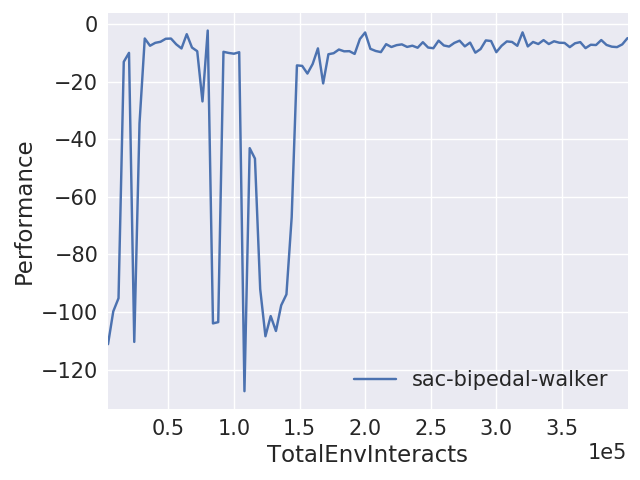
\includegraphics[width=0.91\textwidth]{figures/rl-framework/sac-bipedal-walker.png}
         \caption{Spinning Up implementation (Default parameters) - Goal not achieved in 400.000 steps}
     \end{subfigure}
     \hfill
     \begin{subfigure}[t]{0.49\textwidth}
         \centering
         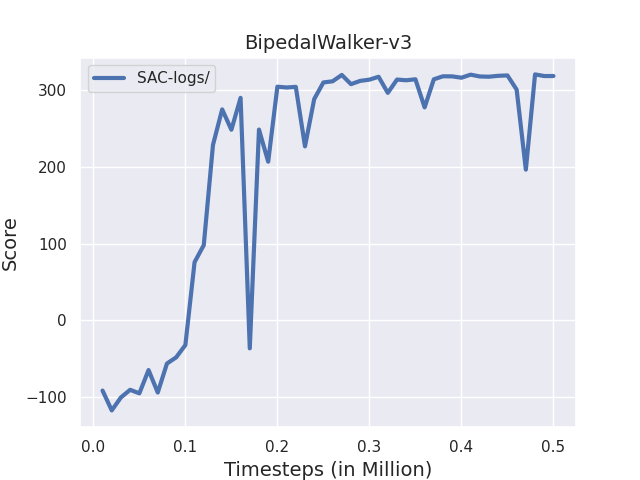
\includegraphics[width=\textwidth]{figures/rl-framework/sb3-sac-BipedalWalker-v3.png}
         \caption{Stable Baselines3 implementation (Tuned parameters) - Goal Achieved in 200.000 steps}
     \end{subfigure}
        \caption{Training Performance of SAC implementations. Goal Score: 300}
        \label{fig:spinup-vs-sb3}
\end{figure}

Moreover, the RL Baselines Zoo has the missing features of Spinning Up's training framework, namely hyperparameter optimization and continuing training of previously trained models \cite{rl-zoo3}. Therefore, Stable Baselines 3 will be the choice of RL Framework.

\section{Custom OpenAI Gym Environment} \label{sec:gym-environment}
In this section, the Reinforcement Learning environment implemented to train the sailboat autopilot will be described.

\subsection{Available data and Environment Constraints}
A good way to train the RL autopilot would be to randomly create goal locations around the boat's initial location, and let the reinforcement learning agent learn how to reach them the fastest way. By setting the initial states and goal locations randomly, the agent would be able to learn how to sail in all possible wind angle and sea state combinations.

Unfortunately, we do not have information about the sea states anywhere except where the boat was in the recorded data. Therefore, the Reinforcement Learning episodes need to happen around the historical boat locations.

\subsection{Core Environment Setup}
There are many different versions of environment that were created. The difference is mostly the observation space of the agent, and the reward function. All of these environments share the rest and the largest part of the code, the core of the environment which will be described here.

As explained in the previous sections, the models are not transferable to other datasets, and we only have sea state data from the historical data from the boat's location. Therefore the \textit{Atlantic} dataset will be used as a baseline for the environment. The main goal of the gym environment is to reach where the historical boat was a few minutes later, and hopefully reach there faster than the historical boat.

\begin{figure}[htbp]
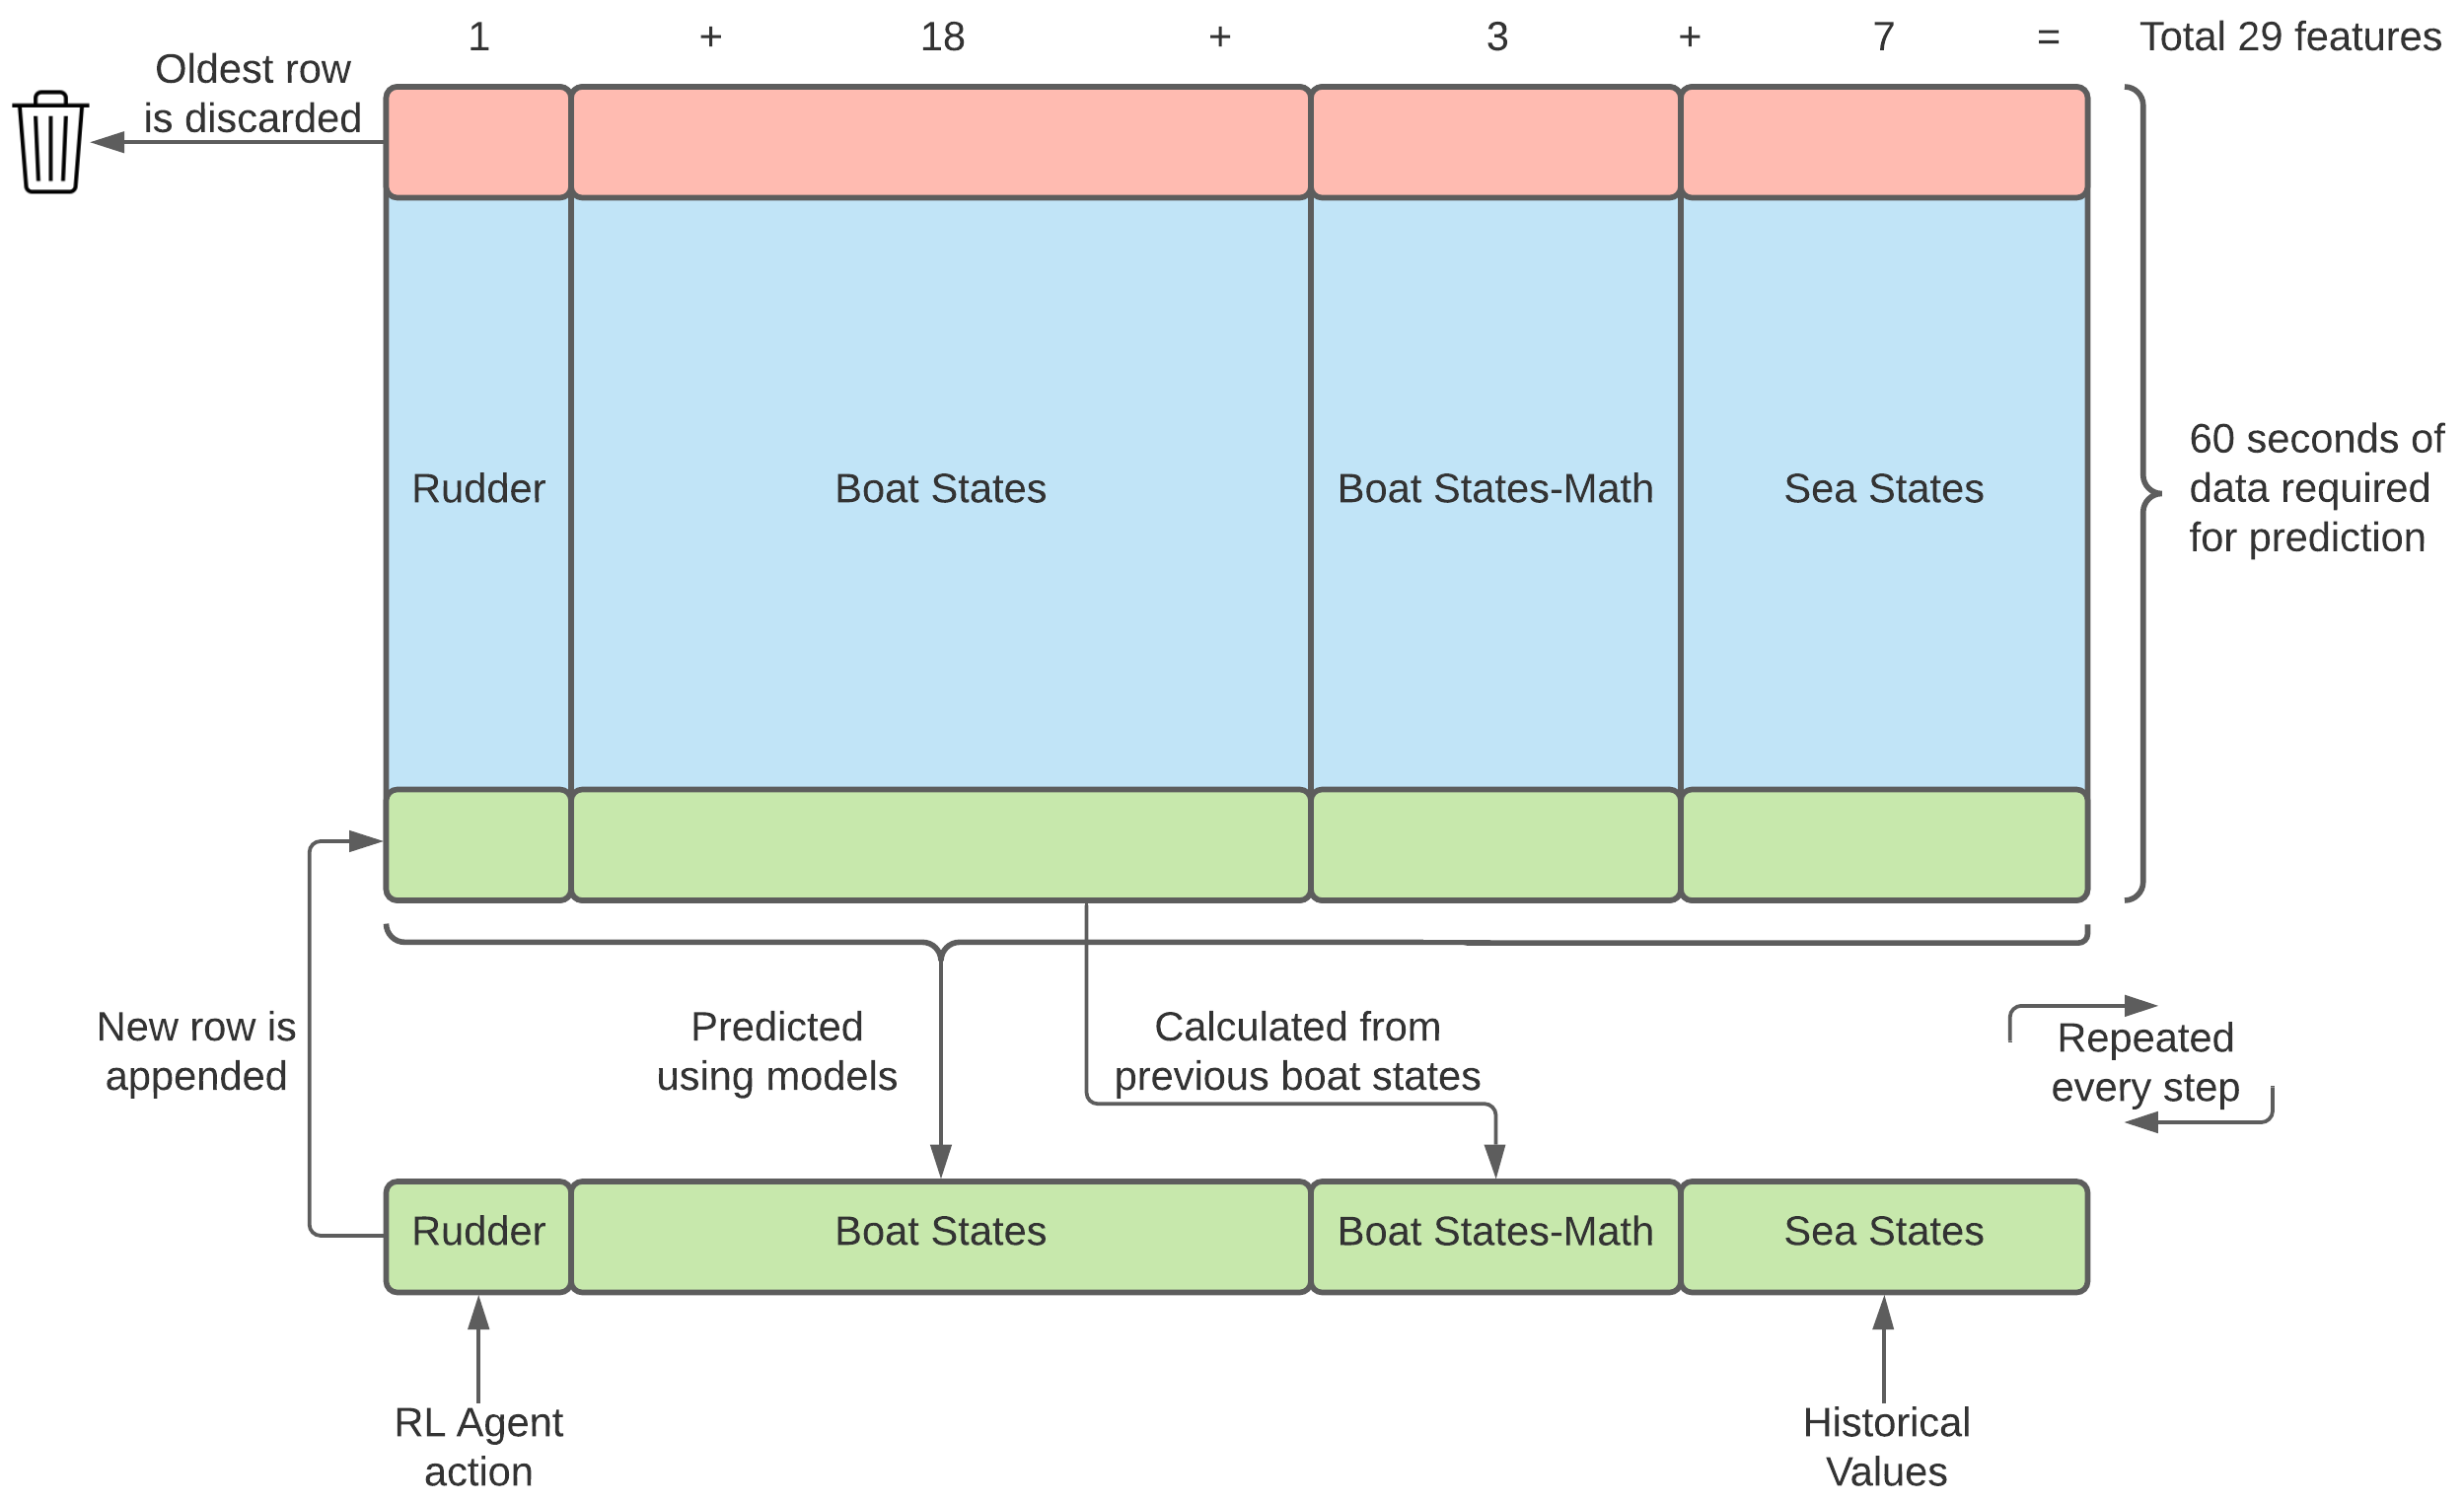
\includegraphics[width=1.1\textwidth,center]{figures/rl-env/JTR env setup.png}
\caption{RL Environment Setup}
\label{fig:env-setup}
\end{figure}

The core gym environment structure, whose diagram can be seen in Figure \ref{fig:env-setup}, is as follows: At the beginning of each episode, a random 60 second section is chosen as the state history from the preprocessed, usuable areas of \textit{Atlantic} dataset. Every timestep, the new row of states are created and appended to the end of the state history, while the oldest row is discarded. This state history contains 4 sections, which are all generated in different ways:

\begin{itemize}
    \item \textbf{Rudder:} The rudder angle. This is provided by the RL agent every step. As the agent learns to drive the boat better, it provides better angles.
    \item \textbf{Boat States:} Features describing the current state of the boat. These 18 states are predicted by the state estimator models, using the 60 seconds of state history.
    \item \textbf{Boat States - Math:} 3 features that are more accurately calculated from previous values mathematically, rather than using ML models, as tested by Charles \cite{charles}.
    \item \textbf{Sea States:} The features that describe the sea state, independent from the boat. These features are taken from the historical values.
\end{itemize}

\noindent The full details of which features every section contains can be found in appendix.

To ensure that the sea states are valid, when the simulated boat diverges too much from the historical route, the environment is reset and another episode is started with new initial states.

\subsection{Gym Environment Rendering}
A visual rendering of the environment have been implemented to better understand and view how the agent performs, which can be seen in Figure \ref{fig:env-render}.

\begin{figure}[htbp]
\centering
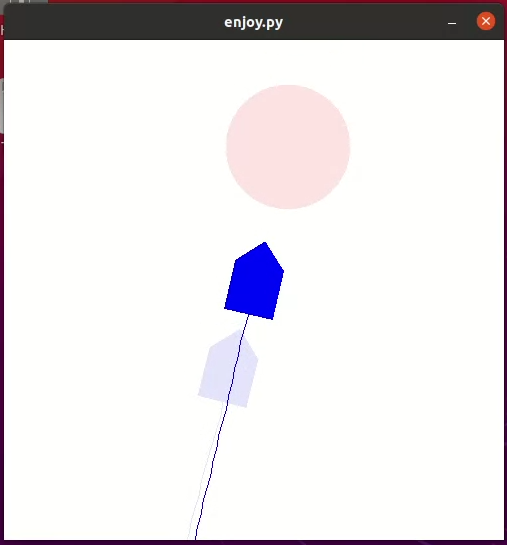
\includegraphics[width = 0.5\hsize]{figures/rl-env/rendering.png}
\caption{Environment Render}
\label{fig:env-render}
\end{figure}

The dark blue boat is the one the RL agent controls in real time, and the dark blue line is the path taken. The light blue counterparts are the historical data that the agent is trying to take over. The light red area is the goal, which the environment is reset when the dark blue boat reaches it. Other useful information such as the speed of the boat, rudder angle provided by the agent, distance to goal, etc. are printed to terminal.

\section{State Estimator Problem}
After the initial versions of the OpenAI Gym Environment have been implemented, they have been trained on Azure Cloud CPUs. The training reward graph for the default Stable Baselines 3 hyperparameters and the popular gSDE hyperparameters for SAC, can be seen in Figure \ref{fig:jtr-v1}.

\begin{figure}[htbp]
\centering
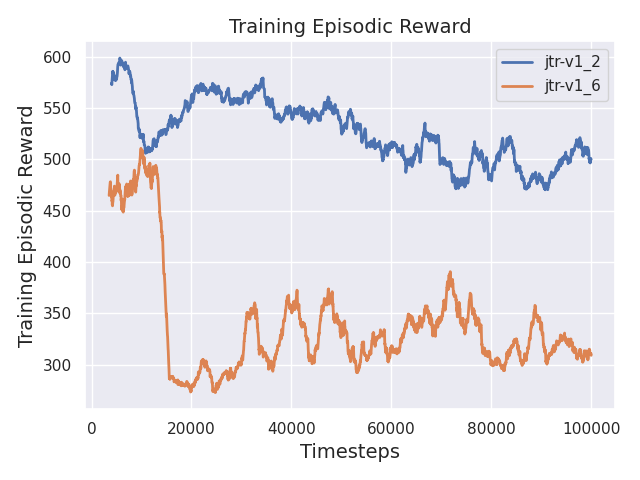
\includegraphics[width = 0.65\hsize]{figures/rl-reward-plots/jtr-v1 100k.png}
\caption{jtr-v1 training plot for default(blue) and gSDE(orange) hyperparams}
\label{fig:jtr-v1}
\end{figure}

There is no improvements in the reward the agent achieves, in 100 thousand steps, the general trend for the reward is downwards, which indicates that there is a problem. To find the problem, the resulting agent from the training run have been observed. The simulation starts fine for the first few seconds, but it very quickly gets problematic. A four second section of the problematic part can be seen in Figure \ref{fig:heading-problem}. 

\begin{figure}[h]
     \centering
     \begin{subfigure}[b]{0.24\textwidth}
         \centering
         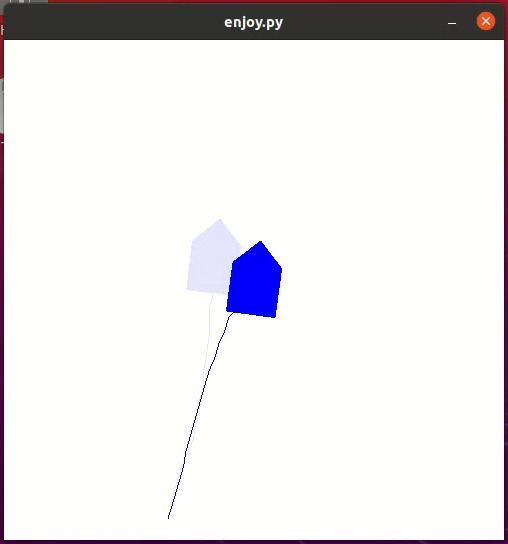
\includegraphics[width=\textwidth]{figures/heading-problem/heading-t0.png}
         \caption{t=0 Rudder=3.4}
     \end{subfigure}
     \begin{subfigure}[b]{0.24\textwidth}
         \centering
         \includegraphics[width=\textwidth]{figures/heading-problem/heading-t1.png}
         \caption{t=1 Rudder=5.1}
     \end{subfigure}
     \begin{subfigure}[b]{0.24\textwidth}
         \centering
         \includegraphics[width=\textwidth]{figures/heading-problem/heading-t2.png}
         \caption{t=2 Rudder=3.3}
     \end{subfigure}
     \begin{subfigure}[b]{0.24\textwidth}
         \centering
         \includegraphics[width=\textwidth]{figures/heading-problem/heading-t3.png}
         \caption{t=3 Rudder=4.5}
     \end{subfigure}
        \caption{Discrepancy between rudder angle and heading}
        \label{fig:heading-problem}
\end{figure}

The possible rudder range is between -50 to 50 degrees. Here, the provided rudder angles are pretty straight, in 3 to 5 degrees range. However, the boat heading is wildly jumping left to right with each step. This indicates that the problem is not on the Reinforcement Learning part, but the state estimator part. Therefore, the state estimator models were examined next.

\subsection{Test 1: Long Term Predictions}

\subsubsection{Current Information}
\begin{itemize}
    \item Previous students have tested how the models perform for the next one time step only.
    \item To use the state estimator models in a Reinforcement Learning setting, the state estimators need to be able to reliably predict values long term, using previously predicted values as input.
\end{itemize}

\subsubsection{Hypothesis}
The state estimator models can successfully make accurate long-term predictions, using previously predicted values as input.

\subsubsection{Experimental Setup}
To test the state estimators, a similar approach to Figure \ref{fig:env-setup} in Core Environment Setup section have been used. The models were given a 60 second history. For every timestep, the historical rudder angle and sea states were used, the new boat states were predicted with the 18 state estimator models, and the remaining 3 boat states were calculated mathematically. For every new prediction for \textit{t+1}, data between \textit{t-59} and \textit{t} were used. 60 seconds of new states were predicted/calculated. The predicted/calculated values were then compared to the historical values.

\begin{figure}[h]
     \centering
     \begin{subfigure}[b]{0.32\textwidth}
         \centering
         \includegraphics[width=\textwidth]{figures/prediction-plots/Rudder.png}
         \caption{Rudder}
     \end{subfigure}
     \begin{subfigure}[b]{0.32\textwidth}
         \centering
         \includegraphics[width=\textwidth]{figures/prediction-plots/TWS.png}
         \caption{TWS (Sea State)}
     \end{subfigure}
     \begin{subfigure}[b]{0.32\textwidth}
         \centering
         \includegraphics[width=\textwidth]{figures/prediction-plots/Current_speed.png}
         \caption{Current\_speed (Sea State)}
     \end{subfigure}
        \caption{Using historical rudder angle and sea states}
        \label{fig:prediction-sea-rudder}
\end{figure}

\subsubsection{Results}
The first 60 seconds are the historical values, the predictions start after 60 seconds. The first few values, in t=61, 62, and 63 are close to the historical values, but very quickly after the first few seconds, the predictions start jumping between very high and very low in every step. A few example features of the 18 predicted states are presented in Figure \ref{fig:prediction-boat-states}. The blue line is the historical values, and the orange line is the predicted values. The plots of all features can be found in Appendix.

\begin{figure}[h]
     \centering
     \begin{subfigure}[b]{0.32\textwidth}
         \centering
         \includegraphics[width=\textwidth]{figures/prediction-plots/AWA_cos.png}
         \caption{AWA\_cos}
     \end{subfigure}
     \begin{subfigure}[b]{0.32\textwidth}
         \centering
         \includegraphics[width=\textwidth]{figures/prediction-plots/AWA_sin.png}
         \caption{AWA\_sin}
     \end{subfigure}
     \begin{subfigure}[b]{0.32\textwidth}
         \centering
         \includegraphics[width=\textwidth]{figures/prediction-plots/AWS.png}
         \caption{AWS}
     \end{subfigure}
     \begin{subfigure}[b]{0.32\textwidth}
         \centering
         \includegraphics[width=\textwidth]{figures/prediction-plots/Speed_ov_ground.png}
         \caption{Speed\_ov\_ground}
     \end{subfigure}
     \begin{subfigure}[b]{0.32\textwidth}
         \centering
         \includegraphics[width=\textwidth]{figures/prediction-plots/VMG.png}
         \caption{VMG}
     \end{subfigure}
     \begin{subfigure}[b]{0.32\textwidth}
         \centering
         \includegraphics[width=\textwidth]{figures/prediction-plots/Yaw_cos.png}
         \caption{Yaw\_cos}
     \end{subfigure}
        \caption{Some of predicted boat states, Historical(Blue) vs Predicted(Orange)}
        \label{fig:prediction-boat-states}
\end{figure}


\subsubsection{Conclusion}
The hypothesis is refuted. The state estimator models cannot successfully make accurate long-term predictions, using previously predicted values as input. Therefore the state estimator models in their current condition are not suitable for simulating a Reinforcement Learning Environment.

\subsubsection{Next Steps}
Yaw\_cos stands out to be the feature that clearly performs very poorly from the first prediction. Further tests will be made by using historical Yaw\_cos, to see if Yaw\_cos was causing the problems in other predictions.

\subsection{Test 2: Problematic feature Yaw\_cos}
\subsubsection{Current Information}
\begin{itemize}
    \item Because the models for each feature uses the predicted values from all the other features in their input, one bad model might affect all the features.
    \item Yaw\_cos clearly stands out as the worst performing model from the very first prediction.
\end{itemize}

\subsubsection{Hypothesis}
The poor predictions of Yaw\_cos is the root cause that affect the inputs of all other features, causing them to make inadequate predictions.

\subsubsection{Experimental Setup}
Same setup with \textit{Test 1: Long term predictions} will be applied, but historical Yaw\_cos values will be used instead of making predictions. Then the outputs of Test 1 and Test 2 will be compared.

\subsubsection{Results}
The results of Test 2(Orange) were drawn in the same plot with the results of Test 1(Green) for an easier comparison. As can be seen in Figure \ref{fig:prediction-Yaw-cos}, the results are very similar to Test 1 results. In some features, the jumps start a little later, and the amplitude of jumps are a little smaller. The plots of all features can be found in Appendix.

\begin{figure}[h]
     \centering
     \begin{subfigure}[b]{0.32\textwidth}
         \centering
         \includegraphics[width=\textwidth]{figures/prediction-plots-compared/AWA_cos.png}
         \caption{AWA\_cos}
     \end{subfigure}
     \begin{subfigure}[b]{0.32\textwidth}
         \centering
         \includegraphics[width=\textwidth]{figures/prediction-plots-compared/AWA_sin.png}
         \caption{AWA\_sin}
     \end{subfigure}
     \begin{subfigure}[b]{0.32\textwidth}
         \centering
         \includegraphics[width=\textwidth]{figures/prediction-plots-compared/AWS.png}
         \caption{AWS}
     \end{subfigure}
     \begin{subfigure}[b]{0.32\textwidth}
         \centering
         \includegraphics[width=\textwidth]{figures/prediction-plots-compared/Speed_ov_ground.png}
         \caption{Speed\_ov\_ground}
     \end{subfigure}
     \begin{subfigure}[b]{0.32\textwidth}
         \centering
         \includegraphics[width=\textwidth]{figures/prediction-plots-compared/VMG.png}
         \caption{VMG}
     \end{subfigure}
     \begin{subfigure}[b]{0.32\textwidth}
         \centering
         \includegraphics[width=\textwidth]{figures/prediction-plots-compared/Yaw_cos.png}
         \caption{Yaw\_cos}
     \end{subfigure}
        \caption{Historical(Blue) vs Test1(Orange) vs Test2(Green)}
        \label{fig:prediction-Yaw-cos}
\end{figure}

\subsubsection{Conclusion}
The hypothesis is refuted. The poor predictions of Yaw\_cos is not the root cause that affects all other features, it is only a small part of the problem. There is no other feature that stands out as clearly as Yaw\_cos as having poor predictions.

\subsubsection{Next steps}
The problem with the state estimators is not something that can be solved quickly. The Reinforcement Learning Gym Environment will be refined assuming a working state estimator model, so it can be used when the state estimators are improved.

\section{OpenAI Gym Environment Refinements}
Examining the results of the State Estimator models, it is clear that they are not suitable for use in a Reinforcement Learning Environment in their current state. Therefore, to refine the Gym Environment, a simple environment with no machine learning models will be used.

To build a basic autopilot, the agent does not need to know the full 28 features present in our data. It only needs 2 features, the speed and the heading of the boat. The gym environment will be refined by assuming a constant speed, and a linear relationship between the rudder and heading, such as if the rudder is turned 10 degrees to left, the boat will turn 10 degrees to left in the next second.

As explained in Core Environment Setup section, the main goal of the gym environment is to reach where the historical boat was a few minutes later, and hopefully reach there faster than the historical boat. The reward function and the observation space of the agent was refined through many iterations to achieve this main goal. The details of what was changed during each iterations, which also include performance and rendering improvements can be seen in Appendix.

\subsection{Observation Space}
To help the agent reach the goal, we need to provide the necessary information to the agent in the observation space. The initial, naive attempt was to include both the current location and the goal location separately in the observation space. Different formats were tried using cos and sin or angular values. Neither of the attempts were successful.

Next, widely used Gym environments were examined. Many of the similar goal oriented Gym Environments such as the Lunar Lander \cite{LunarLander-v2} and the Robotics Environments \cite{gym-robotics} use relative position in their observation space. This makes sense for our environment too, as how the autopilot steers the boat should not change based on latitude and longitude, we only need the relative position information to be able to reach the goal. Therefore, using relative position between the current location and the goal location have been tried, but it wasn't very successful either. 

Finally, the existing autopilots that utilize heading and compass for steering were inspired from, and heading was used in the observation space, which showed great success. The final observation space consists of the current boat heading angle, and the heading angle to the goal location, recalculated at every timestep. 

The speed of the boat, which is crucial for a high performance autopilot, was omitted in the final version as it is constant. The suggested observation space to be used when the state estimators are improved, proposed based on experiences during implementation and sailing domain knowledge can be found in Suggested Environment section.

\subsection{Reward Function}
The reward function Roman used only gave rewards based on how close it is to the historical route. There are no rewards based on speed or time taken. Plus there are no bounds for rewards. The rewards reach hundreds of thousands per episode, which makes judging the agent from rewards difficult. It is clear that we need a better reward function.

The initial inspiration for the reward function was the Car Racing \cite{CarRacing-v0} environment. It is a similar environment to ours in the sense that we are trying to make the vehicle reach the finishing point as fast as possible. The first versions of our environment followed a very similar reward function to the Car Racing environment. There are at most 1000 rewards given, based on how close the boat is able to get to the goal location. Then, there is some penalty based on time, such that if the boat reaches the goal at the same time with the historical boat, the total reward will be 900. If the agent can reach the goal faster, the reward will be more than 900, if it is slower, reward will be less than 900.

Observing the behaviour of the trained agent, a lot of times, the boat was getting close to the goal but not quite reach it, then it was going straight past the goal. As a solution, in addition to the rewards while getting closer to goal, a penalty was added when moving away from the goal. But the total reward for reaching the goal was kept at 1000.

A penalty for rudder movement was experimented with, which helps the agent learn that the quickest route is more or less a straight line. However, there are good rudder movements that makes a boat go faster, so this penalty were removed. More information about this rudder movements can be found in the Suggested Environment Section.

Finally, we wanted to give more weight in rewards for reaching the goal fast, so the reward for reaching the goal was decreased to 200 while keeping the time penalty the same. 

The resulting reward function makes it easy to judge the behavior of the agent from the episode reward. A negative reward means that the boat can't make progress towards the goal. Reward near 100 means that it can reach the goal, but not as fast as the historical boat. Lastly, if the reward is more than 100, the agent can reach the goal faster than the historical boat, and the environment is solved.

\subsection{Final Refined Environment}
jtr-modelless-v4 is the final refined environment, which uses the mentioned observation space and the reward function. The 

\begin{figure}[htbp]
\includegraphics[width=1.1\textwidth,center]{figures/Contribution/jtr-modelless.png}
\caption{Modelless Environment Setup}
\label{fig:modelless-env-setup}
\end{figure}

Using Stable Baselines3's Soft-Actor Critic algorithm with the default hyperparameters, it converges before 15 thousand steps. The trained agent can be watched on \href{https://youtu.be/uccN--r2uc0} {\underline{\textit{YouTube}}}, and the training episode rewards for the final refined model can be seen in Figure \ref{fig:modelless-v4}.

\begin{figure}[h]
    \centering
    \begin{subfigure}[b]{0.48\textwidth}
        \centering
        \includegraphics[width=\textwidth]{figures/rl-refinements/modelless-v4 100k steps.png}
        \caption{Full run for 100k steps}
    \end{subfigure}
    \begin{subfigure}[b]{0.48\textwidth}
        \centering
        \includegraphics[width=\textwidth]{figures/rl-refinements/modelless-v4 zoomed in.png}
        \caption{Zoomed in}
    \end{subfigure}
    \caption{Training episodic reward of final refined environment}
    \label{fig:modelless-v4}
\end{figure}

\section{Suggested Environment}
A successful refined version have been implemented that can consistently reach the goal faster than the historical boat. In order to make use of this environment in the future, a suggested environment was created, to be used when the state estimator models are improved.

Using the state estimators in each step makes the training significantly longer, as each step takes a little less than 1 second. This is pretty slow in reinforcement learning applications. Assuming the improved state estimators will take as long, it is important to make the environment as efficient as possible and not rely on excess computing power.

\subsection{Suggested Observation Space}
To make the environment efficient, the observation space should not contain any unnecessary features. The suggested observation space have been picked, combining sailing domain knowledge and the results of previous environment iterations.

The suggested observation space have 7 features:
\begin{itemize}
    \item \textbf{Speed\_ov\_ground:} Speed is a key factor that will help the agent reach the goal faster than the historical boat.
    \item \textbf{AWS, AWA:} Apparent Wind Speed and Apparent Wind Angle is important, as how you steer the boat differs based on these.
    \item \textbf{Pitch, Roll:} As explained in Elements Affecting Heading section in Sailing Background chapter, boat heel and the waves have a big affect on the heading. Including these in the observation space will allow the agent to learn the relationship with heading and preemptively counteract the affect of waves and heel.
    \item \textbf{Heading\_ov\_ground, Heading to goal:} These two features are ones used in the final refined environment that performed the best.
\end{itemize}

\subsection{Future Implementation}
The suggested environment and an accompanying interface have been created with necessary explanations and methods to be implemented. When the \textit{StateEstimatorSuggested} class is implemented using the improved state estimators that follows the created interface, the suggested environment will be ready to use. See appendix for a user guide on how to use train and observe the agents on the environments.

\section{RL Algorithm Comparisons}
The initial goal was to do the Reinforcement Learning Algorithm comparisons with the environment that uses the state estimator models. However, the state estimator models were problematic, so the refined jtr-modelless-v4 will be used to compare the algorithms which were researched about in the Literature Review section.

SAC with default and gSDE hyperparameters and TQC default stablebaselines3 hyperparameters were compared. You can see the results in Figure \ref{fig:rl-comparison}.

\begin{figure}[h]
    \centering
    \begin{subfigure}[b]{0.48\textwidth}
        \centering
        \includegraphics[width=\textwidth]{figures/rl-reward-plots/modelless-v4-sac.png}
        %\caption{tack \cite{img:sailing-tack-gybe}}
    \end{subfigure}
    \begin{subfigure}[b]{0.48\textwidth}
        \centering
        \includegraphics[width=\textwidth]{figures/rl-reward-plots/modelless-v4-tqc.png}
        %\caption{jibe \cite{img:sailing-tack-gybe}}
    \end{subfigure}
    \caption{Training Reward Comparison of Algorithms on jtr-modelless-v4}
    \label{fig:rl-comparison}
\end{figure}

We can see that SAC with gSDE hyperparameters clearly perform worse than the others. The timesteps needed for convergence, and the maximum reward achieved are both less than default SAC and TQC. 

TQC is known to be especially excelling in harder environments \cite{tqc-paper}. The jtr-modelless-v4 is a pretty easy environment, with converges happening before 15 thousand steps, and there is only so much faster you can go than the historical boat, which makes the reward capped around 110. Still, comparing default SAC and TQC environments, we can see that once SAC reaches convergence, it stays consistent till the end of training; whereas TQC does more exploration, trying to escape a possible local minimum, which gives it the advantage in more challenging environments. 

Therefore, TQC should be incorporated in the future environments using state estimator models. If the improved state estimators are able to successfully replicate the real sea environment, there will be a lot of nuances to be learned by the RL agent. Such as when and how much to move the rudder compared to the observed features of pitch, roll, wind, etc, to keep the boat speed maximum and reach the in the fastest way.

%%%%%%%%%%%%%%%%%%%%%%%%%%%%%%%%%%%%
\chapter{Conclusion}

\section{Outcomes}
TBC: Compare with objectives in Introduction, what was achieved what was not. Highlight successes and shortcomings.

\section{Future Work} \label{sec:future-work}
TBC: Explain future work and show pointers to main body where they were mentioned.

\section{Ethical Considerations}
TBC

%% bibliography
\bibliographystyle{unsrt}
%\setlength\bibsep{3pt}
\bibliography{bibliography}


%% appendix
\appendix
\addtocontents{toc}{\protect\setcounter{tocdepth}{0}}

\chapter{Ethics Checklist}
TBC

\chapter{Sail Trim Approach}
In this chapter, a proposed extension to the broader "Automation and Intelligent Optimisation in High Performance Sailing Boats" project will be described. This Sail Trim Approach was my proposed master's thesis topic, but together with my supervisors, we decided to continue the Reinforcement Learning Approach instead.

\section{Introduction}
Sail trim is the biggest factor in the speed of the boat. An autopilot with a good sail trim would go faster than an expert human skipper with a bad sail trim. With a camera at the back of the boat looking at the main sail, we can train a model that can predict whether the main sail trim is good, too loose, or too tight.

Judging the sail trim is easy to a trained eye, but depending on the wind conditions, might require a lot of attention if the wind is gusty, or there is land or any obstacles nearby that might disturb the wind flow.
 
Full crews have dedicated people for sail trim, however it is hard to achieve constant good trim with shorthanded sailing with one or two people. This project would help shorthanded sailors, for cruising or racing, plus it can also be used for teaching sail trim to beginners.


\section{Literature Review}
In this section, a current overview of the relevant topics related to the proposed Sail Trim Approach (\ref{LR:TL}, \ref{LR:IG}, and \ref{LR:AST}) are presented. Transfer Learning is a suggested technique to be used in Sail Trim Approach so that the model can be trained with less collected data. Integrated Gradients is an Explainable AI technique which can be used for understanding what the sail trim model is learning to check if its correct. Lastly, Assisted Sail Trim is a system used in cruising yachts that is somewhat similar to the proposed Sail Trim Approach.

\subsection{Transfer Learning} \label{LR:TL}
Transfer learning is a method where a machine learning model trained for a task is used as a starting point for another task.\cite{brownlee_2019} In our context, instead of training a model from ground up, transfer learning can be utilized by building up on a model that was previously trained for a large scale image classification task. The idea behind transfer learning for imaging is that if a model is trained on a large and general enough dataset, it can serve as a generic model of the visual world. \cite{TF:TL} This generic model can be trained much more easily to classify different sail trims thanks to its advantages. 

Lisa Torrey and Jude Shavlik explain in their book the 3 advantages of transfer learning and how it improves model learning \cite{10.5555/1803899}, which can be seen in Figure \ref{fig:TL}.

\begin{figure}[h]
\centering
\includegraphics[width = 0.7\hsize]{figures/transfer-learning.png}
\caption{Transfer learning performance improvements \cite{10.5555/1803899}}
\label{fig:TL}
\end{figure}

\begin{enumerate}
  \item \textbf{Higher start:} The initial performance is better 
  \item \textbf{Higher slope:} The model improves faster 
  \item \textbf{Higher asymptote:} The converged performance is better 
\end{enumerate}

\begin{figure}[h]
\centering
\includegraphics[width = 0.7\hsize]{figures/transfer learning results.png}
\caption{Affect of transfer learning on accuracy vs sample size \cite{ZHU2021104269}}
\label{fig:TL-results}
\end{figure}

Theoretically, using transfer learning the deep learning models converge much faster, as seen in Figure \ref{fig:TL}. This means that models can be trained with a lot less data. In their study, Wenbo et al. examines the transfer learning for image classification's impact on training sample size. \cite{ZHU2021104269} Wenbo et al. conclude that the deep learning models can achieve over 90\% accuracy for image classification tasks by using less than 100 samples utilizing transfer learning, significantly lower than the previous rule of thumb of 1000 samples per class. Wenbo et al.'s results graph of accuracy vs sample size, with and without transfer learning can be seen in Figure \ref{fig:TL-results}.

\subsection{Integrated Gradients} \label{LR:IG}
Integrated Gradients is an explainable AI technique to help understand what the model is learning, which can be used in any differentiable model such as images, text or structured data. \cite{TF:IG} The suggested usage in the sail trim approach is on images, to see whether the model is learning the expected features. The technique is easy to implement, and requires no modifications on the original network, only requires some calls to the standard gradient operator. \cite{IGpaper} An example of Integrated gradients used on images can be seen in Figure \ref{fig:IG}. 

\begin{figure}[h]
\centering
\includegraphics[width = 0.7\hsize]{figures/IG_fireboat.png}
\caption{Integrated Gradients example \cite{TF:IG}}
\label{fig:IG}
\end{figure}

When the models do not perform as expected, or just to see what the models have learned, Integrated Gradients is a nice technique to have to be able to understand and debug the models: either by regularization or gathering more and better balanced data.

\subsection{Jeanneau \& Harken Assisted Sail Trim} \label{LR:AST}
A somewhat similar idea to the sail trim approach has been done as a collaboration with Jeanneau and Harken in 2015, \cite{harkenAST} which won the Pittman Innovation Award. \cite{pittman_awards}
The Assisted Sail Trim (AST) system has several components. The relevant component to this project focuses on maintaining the rough trim of the sails by adjusting the sheets depending on the apparent wind measured by on-board electronics. An illustration of this can be seen in Figure~\ref{fig:AST}.

\begin{figure}[h]
\centering
\includegraphics[width = \hsize]{figures/AST.png}
\caption{Assisted Sail Trim - apparent wind sail adjustment \cite{ASTbrochure}}
\label{fig:AST}
\end{figure}

AST is only available on the 2015 Jeanneau Sun Odyssey 519, and it is discontinued. It also did not utilize machine learning, required much more electronics and budget than a single camera, and it was specific to the sailboat, not transferable. In addition, the sails can have vastly different shapes even in similar sheet positions, resulting in great performance difference. The proposed sail trim approach focuses on the fine sail trim, rather than the coarse trim achieved in AST.

Another difference between AST and the suggested sail trim approach is that AST system can communicate with the winches, and automatically adjust the main sheet. Suggested sail trim approach will not communicate with the rest of the onboard electronics, and rely on the crew to take actions. Although this is less user friendly, it has its own advantages. Two use cases of the sail trim approach are education and competition. Making the crew do the trim by giving trim suggestion will be more educational than doing it for them. Plus automated sail trim is not allowed in some class rules, so this project can be used in competitions among wider sailboat classes.

\section{Sail Trim Background}
As explained in section \ref{LR:AST}, the sails can have vastly different shapes in similar boom and sheet positions as can be seen in Figure~\ref{fig:mainsail-trim}. There are a lot of reasons why a sail trim might be off. For example the sail might not be cut properly, or the mast position and mast bend might not be optimal for the weather conditions. But these are pretty unlikely, and most likely, it is the mainsail controls that can be adjusted on the go that cause bad trim. Below are some notable reasons of bad mainsail trim on the go.

\begin{figure}[h]
\centering
\includegraphics[width = 0.6\hsize]{figures/sail-trim-approach/mainsail-trim-back.jpg}
\caption{Good(left) and bad(right) light wind mainsail trim \cite{img:mainsail-trim-back}}
\label{fig:mainsail-trim}
\end{figure}

\noindent Main sail might be too strained because of:
\begin{itemize}
  \item The main sheet is pulled in too much
  \item Boom vang is too tight
  \item Main sail traveller is not utilized correctly
\end{itemize}

\noindent Main sail might be too loose because of:
\begin{itemize}
  \item The main sheet is not pulled enough
  \item Boom vang is too loose
  \item Main sail is not fully up to the top of the mast
\end{itemize}

There are other mainsail controls that affect the trim such as cunningham and outhaul, but those depend a lot on the boat class, and even in same boat class, different sailmakers have different suggestions on how to utilize them. The mentioned mainsail controls can be seen in Figure \ref{fig:mainsail-controls}.

\begin{figure}[h]
\centering
\includegraphics[width = 0.7\hsize]{figures/sail-trim-approach/mainsail-shape-controls.png}
\caption{Mainsail controls that affect trim \cite{img:mainsail-shape-controls}}
\label{fig:mainsail-controls}
\end{figure}

\section{Sail Trim Capture System}

The suggested camera placement is at the center back of the boat, possibly at the bimini top, as shows in Figure \ref{fig:camera-pos}. A camera from this angle will see a similar view of the sails with Figure \ref{fig:telltales}.

\begin{figure}[h]
\centering
\includegraphics[width = 0.7\hsize]{figures/sail-trim-approach/camera-position.png}
\caption{Camera position}
\label{fig:camera-pos}
\end{figure}

\begin{figure}[h]
\centering
\includegraphics[width = 0.8\hsize]{figures/sail-trim-approach/telltales.jpg}
\caption{Camera's view of a bad(left) and good(right) light wind mainsail trim \cite{img:telltales}}
\label{fig:telltales}
\end{figure}

The easiest way to tell if the trim is good for a human is to look at the red telltales at the back of the sails, see Figure \ref{fig:telltales}. The most important one is the topmost one. If the telltales are flying straight back, it means that the air is coming out of the sails alright. However if the telltale is going to the back of the sails, it shows us that the wind flow at the back of the sails are not optimal, meaning the trim is sub-optimal and the sails need to be loosened.

For a machine, the easiest way to check trim might be comparing the areas of sail and the sky. In Figure \ref{fig:telltales}, you'll notice that Assuming a clear sky, by only comparing the number of blue pixels(sky) and the number of whiter pixels(sails), a very simple model can tell the difference between a good and a bad trim.

Using the state of the art image classification models, we can achieve much better results, theoretically learning the sail trim for different wind and weather conditions, apparent wind angles, maybe even across different boats.


\section{Suggested Timeline}

The suggested timeline and some additional details for this project, planned considering the available time for Imperial MSc thesis projects can be seen in Figures \ref{fig:sta-plan1} and \ref{fig:sta-plan2}.

\begin{figure}[h]
\centering
\includegraphics[width = \hsize]{figures/sail-trim-approach/plan1.png}
\caption{Suggested plan - Iterations 1 and 2}
\label{fig:sta-plan1}
\end{figure}

Iteration 1 aims to build a simple Proof of Concept that machine learning models can classify good and bad sail trims. After the initial Proof of Concept, the models are extended in Iteration 2. If the expected results are not met in the first iteration, using Integrated Gradients explained in section \ref{LR:IG}, one can see what the models have learned, assess if the learnt features are correct, and balance the dataset with more data countering the false features.

\begin{figure}[h]
\centering
\includegraphics[width = \hsize]{figures/sail-trim-approach/plan2.png}
\caption{Suggested plan - Iterations 3 and 4}
\label{fig:sta-plan2}
\end{figure}

Iteration 3 aims to implement the models live on-board using a smartphone, including two different interfaces for education and professional use cases. Iteration 4 contains a buffer week if anything goes wrong for the project, then some time for project submission preparations, namely the code submission to software archive, final report, and the final presentation.

For more information about the Sail Trim Approach, you can email me at:\\
\href{mailto:doruktaneli97@gmail.com}{doruktaneli97@gmail.com}

\chapter{Azure State Estimator Training Runs Details} \label{app:azure-runs}

Below are the details of the Azure Cloud GPU runs, including optimization times, training times, error metrics, and the resulting hyperparameters for all features. 3 NVIDIA Telsa K80 GPUs were used in parallel for optimization and training. There are 18 models in total that were created, each GPU optimized and trained 6 models. The runs were started together on 16 June 2021, 08:00.

\medskip

\begin{itemize}
  \item \textbf{GPU-1:} Parts 1 and 5. Stopped on 24 June 2021, 15:00
  \item \textbf{GPU-2:} Parts 2 and 6. Stopped on 25 June 2021, 16:00
  \item \textbf{GPU-3:} Parts 3 and 4. Stopped on 24 June 2021, 15:00
\end{itemize}

\bigskip

\begin{figure}[h]
\centering
\includegraphics[width = \hsize]{figures/Contribution/gpu-runs/part1.png}
\caption{GPU runs - Part 1}
\end{figure}

\begin{figure}[h]
\centering
\includegraphics[width = \hsize]{figures/Contribution/gpu-runs/part2.png}
\caption{GPU runs - Part 2}
\end{figure}

\begin{figure}[h]
\centering
\includegraphics[width = \hsize]{figures/Contribution/gpu-runs/part3.png}
\caption{GPU runs - Part 3}
\end{figure}

\begin{figure}[h]
\centering
\includegraphics[width = \hsize]{figures/Contribution/gpu-runs/part4.png}
\caption{GPU runs - Part 4}
\end{figure}

\begin{figure}[h]
\centering
\includegraphics[width = \hsize]{figures/Contribution/gpu-runs/part5.png}
\caption{GPU runs - Part 5}
\end{figure}

\begin{figure}[h]
\centering
\includegraphics[width = \hsize]{figures/Contribution/gpu-runs/part6.png}
\caption{GPU runs - Part 6}
\end{figure}

\chapter{Charles' Suggested Features Describing the Environment}
\label{app:essential-features}
These 4 features were used while creating the \textit{RDR\_nkz (Atlantic Conditions)} dataset. They are included here for convenience. Below are the explanation of the 4 features, exactly as written in his project report by Charles Metz \cite{charles}:

\subsubsection{Features describing the physical environment} 
Only some features are relevant to describe the physical environment and state of the boat. Indeed, some features are partially redundant to others and some correlate strongly to others (e.g. boat and wind speed under normal conditions). Therefore, 4 features were selected that capture the essential elements of the environment as experienced by the boat. In consultation with Dr. Eric Topham, internal supervisor of the study with extensive sailing experience, these features were found to be: 

\begin{itemize}
    \item \textbf{True Wind Speed (TWS):} important for the lift generated from the airflow over the sails, as well as affecting the sea state.
    \item \textbf{True Wind Angle (TWA):} the angle at which the wind hits the boat in relation to its orientation when the boat would be stationary. It allows to characterize the angle of the wind in relation to the boat at any given moment.
    \item \textbf{Apparent Wind Angle (AWA):} characterizes the angle at which the wind effectively hits the boat when the boat is in motion.
    \item \textbf{Pitch:} describes the inclination of the boat’s bow; numerous high and low values for pitch hence indicate an agitated sea that would raise and lower the nose of the boat. Out of the pitch, roll and yaw angles that describe the attitude of the boat, pitch is the best for approximating the sea state. Indeed, roll can be affected by wind which can be independent of the sea state, and yaw can be affected by the helmsman steering the boat in a choice of direction unrelated to the sea state.
\end{itemize}

\chapter{Creating the RDR\_nkz\_Atlantic\_Conditions Dataset}
The \textit{RDR\_nkz (Atlantic Conditions)} dataset was created by selecting parts of \textit{RDR\_nkz} dataset which have the 4 essential features in the range of what is present in the \textit{Atlantic} dataset.

First, for each feature, the \textit{Atlantic} distribution was checked to see in which value range the models were trained on. Then, the \textit{RDR\_nkz} plot was inspected, to determine candidate sections where the values were in the training range. Later, the sections where the candidates intersect for all features were chosen, and then concatenated to produce the \textit{RDR\_nkz (Atlantic Conditions)} dataset.

The gaps seen in the \textit{RDR\_nkz (Atlantic Conditions)} graphs below are for visualization. There are no long gaps in the new dataset, the remaining parts were concatenated together.

\clearpage
\subsubsection{True Wind Speed (TWS)}
The whole range of \textit{RDR\_nkz} is covered in the training set.

\begin{figure}[h]
\centering
\includegraphics[width = \hsize]{figures/distributions/atlantic-TWS.png}
\caption{Distribution of True Wind Speed in \textit{Atlantic} dataset \cite{charles}}
\end{figure}

\begin{figure}[h]
     \centering
     \begin{subfigure}[t]{0.49\textwidth}
         \centering
         \includegraphics[width=\textwidth]{figures/distributions/RDR-TWS.png}
         \caption{RDR\_nkz}
     \end{subfigure}
     \hfill
     \begin{subfigure}[t]{0.49\textwidth}
         \centering
         \includegraphics[width=\textwidth]{figures/distributions/RDR-atlantic-TWS.png}
         \caption{RDR\_nkz (Atlantic Conditions)}
     \end{subfigure}
        \caption{True Wind Speed plots}
\end{figure}

\clearpage
\subsubsection{True Wind Angle (TWA)}
Again, pretty much all wind angles are covered in training data. However, we have less data from +150 compared to 50 and -150.
To exclude +150 range, Remaining good candidates are:
\begin{itemize}
    \item start-0.45
    \item 0.55-0.75*
    \item 0.8-0.9*
    \item 1.25-end*
\end{itemize}
The candidates that are suitable for all features are shown with a star(*).

\begin{figure}[h]
\centering
\includegraphics[width = \hsize]{figures/distributions/atlantic-TWA.png}
\caption{Distribution of True Wind Angle in \textit{Atlantic} dataset \cite{charles}}
\end{figure}

\begin{figure}[h]
     \centering
     \begin{subfigure}[t]{0.49\textwidth}
         \centering
         \includegraphics[width=\textwidth]{figures/distributions/RDR-TWA.png}
         \caption{RDR\_nkz}
     \end{subfigure}
     \hfill
     \begin{subfigure}[t]{0.49\textwidth}
         \centering
         \includegraphics[width=\textwidth]{figures/distributions/RDR-atlantic-TWA.png}
         \caption{RDR\_nkz (Atlantic Conditions)}
     \end{subfigure}
        \caption{True Wind Angle plots}
\end{figure}

\clearpage
\subsubsection{Apparent Wind Angle (AWA)}
All of the apparent wind angles in \textit{RDR\_nkz} are covered in training data.

\begin{figure}[h]
\centering
\includegraphics[width = \hsize]{figures/distributions/atlantic-AWA.png}
\caption{Distribution of Apparent Wind Angle in \textit{Atlantic} dataset \cite{charles}}
\end{figure}

\begin{figure}[h]
     \centering
     \begin{subfigure}[t]{0.49\textwidth}
         \centering
         \includegraphics[width=\textwidth]{figures/distributions/RDR-AWA.png}
         \caption{RDR\_nkz}
     \end{subfigure}
     \hfill
     \begin{subfigure}[t]{0.49\textwidth}
         \centering
         \includegraphics[width=\textwidth]{figures/distributions/RDR-atlantic-AWA.png}
         \caption{RDR\_nkz (Atlantic Conditions)}
     \end{subfigure}
        \caption{Apparent Wind Angle plots}
\end{figure}

\clearpage
\subsubsection{Pitch}
We want Pitch to be mostly between 0 and 15. Good candidates for this range:
\begin{itemize}
    \item 0.55-0.7*
    \item 0.8-0.9*
    \item 1.25-end*
\end{itemize}
The candidates that are suitable for all features are shown with a star(*).

\begin{figure}[h]
\centering
\includegraphics[width = \hsize]{figures/distributions/atlantic-Pitch.png}
\caption{Distribution of Pitch in \textit{Atlantic} dataset \cite{charles}}
\end{figure}

\begin{figure}[h]
     \centering
     \begin{subfigure}[t]{0.49\textwidth}
         \centering
         \includegraphics[width=\textwidth]{figures/distributions/RDR-Pitch.png}
         \caption{RDR\_nkz}
     \end{subfigure}
     \hfill
     \begin{subfigure}[t]{0.49\textwidth}
         \centering
         \includegraphics[width=\textwidth]{figures/distributions/RDR-atlantic-Pitch.png}
         \caption{RDR\_nkz (Atlantic Conditions)}
     \end{subfigure}
        \caption{Pitch plots}
\end{figure}


\chapter{Boat and Sea States Details}
\subsubsection{Boat States}
Features describing the current state of the boat. These 18 states are predicted by the state estimator models, using the 60 seconds of state history.

\begin{itemize}
    \item AWS (Apparent Wind Speed)
    \item AWA\_cos, AWA\_sin (Apparent Wind Angle)
    \item TWA\_cos, TWA\_sin (True Wind Angle)
    \item Heading\_ov\_ground\_cos, Heading\_ov\_ground\_sin (Heading over ground)
    \item Heading\_Mag\_cos, Heading\_Mag\_sin (Magnetic heading)
    \item Heading\_True\_cos, Heading\_True\_sin (True heading)
    \item Speed\_ov\_ground (Speed over ground)
    \item Speed\_ov\_surface (Speed over surface)
    \item VMG (Velocity Made Good)
    \item Yaw\_cos, Yaw\_sin, Pitch, Roll (3 dimensions of boat movement)
\end{itemize}


\bigskip
\subsubsection{Boat States - Math}
3 features that are more accurately calculated from previous values mathematically, rather than using ML models, as tested by Charles \cite{charles}.

\begin{itemize}
    \item Latitude
    \item Longitude\_cos, Longitude\_sin
\end{itemize}


\clearpage
\subsubsection{Sea States}
The features that describe the sea state, independent from the boat.

\begin{itemize}
    \item Current\_speed (Speed of ocean current)
    \item Current\_direction\_cos, Current\_direction\_sin (Direction of ocean current)
    \item TWS (True Wind Speed)
    \item TWD\_cos, TWD\_sin (True Wind Direction)
    \item Air\_temp (Air temperature)
\end{itemize}


\chapter{State Estimator Tests Prediction Plots}
All of the plots produced for the State Estimator Practicality Tests. The predictions start at the 60 second mark. The blue line is the historical data, orange line is the results of Test 1 which are regular predictions, green line is the results of Test 2 which are predictions using historical Yaw\_cos.

\begin{figure}[ht]
     \centering
     \begin{subfigure}[b]{0.32\textwidth}
         \centering
         \includegraphics[width=\textwidth]{figures/prediction-plots-compared/AWA_cos.png}
         \caption{AWA\_cos}
     \end{subfigure}
     \begin{subfigure}[b]{0.32\textwidth}
         \centering
         \includegraphics[width=\textwidth]{figures/prediction-plots-compared/AWA_sin.png}
         \caption{AWA\_sin}
     \end{subfigure}
     \begin{subfigure}[b]{0.32\textwidth}
         \centering
         \includegraphics[width=\textwidth]{figures/prediction-plots-compared/AWS.png}
         \caption{AWS}
     \end{subfigure}
     \begin{subfigure}[b]{0.32\textwidth}
         \centering
         \includegraphics[width=\textwidth]{figures/prediction-plots-compared/Heading_Mag_cos.png}
         \caption{Heading\_Mag\_cos}
     \end{subfigure}
     \begin{subfigure}[b]{0.32\textwidth}
         \centering
         \includegraphics[width=\textwidth]{figures/prediction-plots-compared/Heading_Mag_sin.png}
         \caption{Heading\_Mag\_sin}
     \end{subfigure}
     \begin{subfigure}[b]{0.32\textwidth}
         \centering
         \includegraphics[width=\textwidth]{figures/prediction-plots-compared/Heading_ov_ground_cos.png}
         \caption{Heading\_ov\_ground\_cos}
     \end{subfigure}
     \begin{subfigure}[b]{0.32\textwidth}
         \centering
         \includegraphics[width=\textwidth]{figures/prediction-plots-compared/Heading_ov_ground_sin.png}
         \caption{Heading\_ov\_ground\_sin}
     \end{subfigure}
     \begin{subfigure}[b]{0.32\textwidth}
         \centering
         \includegraphics[width=\textwidth]{figures/prediction-plots-compared/Heading_True_cos.png}
         \caption{Heading\_True\_cos}
     \end{subfigure}
     \begin{subfigure}[b]{0.32\textwidth}
         \centering
         \includegraphics[width=\textwidth]{figures/prediction-plots-compared/Heading_True_sin.png}
         \caption{Heading\_True\_sin}
     \end{subfigure}
        \caption{Historical(Blue) vs Test1(Orange) vs Test2(Green)}
        \label{fig:prediction-full-1}
\end{figure}

\begin{figure}[ht]\ContinuedFloat
     \centering
     \begin{subfigure}[b]{0.32\textwidth}
         \centering
         \includegraphics[width=\textwidth]{figures/prediction-plots-compared/Speed_ov_ground.png}
         \caption{Speed\_ov\_ground}
     \end{subfigure}
     \begin{subfigure}[b]{0.32\textwidth}
         \centering
         \includegraphics[width=\textwidth]{figures/prediction-plots-compared/Speed_ov_surface.png}
         \caption{Speed\_ov\_surface}
     \end{subfigure}
     \begin{subfigure}[b]{0.32\textwidth}
         \centering
         \includegraphics[width=\textwidth]{figures/prediction-plots-compared/TWA_cos.png}
         \caption{TWA\_cos}
     \end{subfigure}
     \begin{subfigure}[b]{0.32\textwidth}
         \centering
         \includegraphics[width=\textwidth]{figures/prediction-plots-compared/TWA_sin.png}
         \caption{TWA\_sin}
     \end{subfigure}
     \begin{subfigure}[b]{0.32\textwidth}
         \centering
         \includegraphics[width=\textwidth]{figures/prediction-plots-compared/VMG.png}
         \caption{VMG}
     \end{subfigure}
     \begin{subfigure}[b]{0.32\textwidth}
         \centering
         \includegraphics[width=\textwidth]{figures/prediction-plots-compared/Yaw_cos.png}
         \caption{Yaw\_cos}
     \end{subfigure}
     \begin{subfigure}[b]{0.32\textwidth}
         \centering
         \includegraphics[width=\textwidth]{figures/prediction-plots-compared/Yaw_sin.png}
         \caption{Yaw\_sin}
     \end{subfigure}
        \caption{Historical(Blue) vs Test1(Orange) vs Test2(Green)}
        \label{fig:prediction-full-2}
\end{figure}

\begin{figure}[ht]
     \centering
     \begin{subfigure}[b]{0.32\textwidth}
         \centering
         \includegraphics[width=\textwidth]{figures/prediction-plots-compared/Latitude.png}
         \caption{Latitude}
     \end{subfigure}
     \begin{subfigure}[b]{0.32\textwidth}
         \centering
         \includegraphics[width=\textwidth]{figures/prediction-plots-compared/Longitude_cos.png}
         \caption{Longitude\_cos}
     \end{subfigure}
     \begin{subfigure}[b]{0.32\textwidth}
         \centering
         \includegraphics[width=\textwidth]{figures/prediction-plots-compared/Longitude_sin.png}
         \caption{Longitude\_sin}
     \end{subfigure}
        \caption{Plots of features mathematically calculated from previous values}
        \label{fig:prediction-math}
\end{figure}

\chapter{OpenAI Gym Environment All Iterations}
TBC: Add training reward plots

\subsection*{jtr\_env\_v0}
Replicates Roman's reinforcement learning setup while following the gym interface.

\subsection*{jtr\_env\_v1}
Reward function inspired from CarRacing-v0 \cite{CarRacing-v0} that is capped at 1000.
Reduced observation space with 6 features: 
\begin{itemize}
    \item Speed\_ov\_ground
    \item Heading\_ov\_ground\_cos, Heading\_ov\_ground\_sin,
    \item  Relative Latitude, Relative Longitude\_cos, Relative Longitude\_sin
\end{itemize}
The last 3 features are relative position between the current boat position and the goal position.

\subsection*{jtr\_env\_v1\_parallel}
jtr\_env\_v1 parallelized with Joblib using shared memory. Uses more resources but runs slower than jtr\_env\_v1.

\subsection*{jtr\_env\_her\_v0}
Attempt to make use of Hindsight Experience Replay \cite{her-paper} which makes goal oriented environments more efficient. It gives and error, and could not be run due to lack of documentation ro examples of Hinsight Experince Replay functions and how they are called.

\subsection*{jtr\_env\_modelless\_v0}
First iteration of the modelless environments. Does not use any state estimator models. The speed is constant through the episode, and it is equal to the average of the previous 30 seconds, rounded up to the 4th decimal point. The heading is calculated directly from rudder, such that if the rudder is turned right 10 degrees, the heading will turn right 10 degrees in the next second.

Same observation space with jtr\_env\_v1.

-300 penalty for not reaching the goal, and reset the environment if taking too long to reach goal.

\subsection*{jtr\_env\_modelless\_v1}
Simplify the observation space to 4 features:
\begin{itemize}
    \item Speed\_ov\_ground
    \item Heading\_ov\_ground as angle,
    \item Relative Latitude and Longitude as angle
\end{itemize}

\subsection*{jtr\_env\_modelless\_v2}
Remove reward when moving away from the goal, add penalty for rudder angles. The penalty for rudder angles helped the agent to learn that the going straight is faster.

\subsection*{jtr\_env\_modelless\_v3}
First environment that can reach the goal consistently!

Inspired from existing autopilot systems, further simplify the observation space to 2 features:
\begin{itemize}
    \item Heading\_ov\_ground,
    \item Heading required to reach the goal at that timestep.
\end{itemize}
Speed was removed as it is constant through the episode. Latitude and Longitude were removed as those should not affect how the agent steers the boat.

\subsection*{jtr\_env\_modelless\_v4}
Remove rudder penalties as they are necessary to make the boat go faster in real life.

Update the reward function, reaching to goal reduced to 200 from 1000. Reward penalty for not reaching the goal at the end the episode changed to -50 from -300.

Finishing at the same time with the historical boat is 100. Solved is >100, which means the agent can reach the goal faster than historical boat.

Converges in less than 15 thousand step with both SAC and TQC algorithms. Can consistently reach the goal faster than the historical boat.

\chapter{Reinforcement Learning User Guide}
TBC

\end{document}
